\documentclass[a4paper,11pt]{refrep}

\usepackage[utf8]{inputenc}
\usepackage[portuguese]{babel}

% Set the title
\title{Manual do Usuário}

% Font selection
\usepackage{helvet}
\renewcommand{\familydefault}{\sfdefault}
\fontfamily{phv}\selectfont

% Set the page title
\newcommand{\mycontent}[0]{
\begin{tabular}{l}
\hspace*{-6cm} \em XCSoar User Manual \vspace*{2pt}
\end{tabular}}

% Define some xc doc styles
\usepackage{color}

\usepackage{booktabs}
\usepackage{longtable}
\usepackage{rotating}
\usepackage{multicol}
\usepackage{multirow}
\usepackage[disable]{todonotes}
\usepackage[colorlinks=true]{hyperref}
\usepackage{gensymb}
\usepackage{makeidx}\makeindex
\makeatletter
\usepackage{fancyhdr}
\pagestyle{fancy}
\maxipagerulefalse
%
% Include XCSoar header and footer settings and used buttons 

% Add XCSoar User Manual title to the header
\settototalheight\headheight{\mycontent}
\fancyhead[L]{{\mycontent}}

% Add page number to the footer (centered)
\fancyfoot{}
\fancyfoot[R]{\thepage}

% No line between content and header
\renewcommand{\headrulewidth}{0pt}

\fancypagestyle{plain}{
  % Clear fancy header and footer
  \fancyhf{}

  % Add page number to the footer (centered)
  \fancyfoot[R]{\thepage}

  % No line between content and header
  \renewcommand{\headrulewidth}{0pt}
}

% Colors
\definecolor{buttongray}{rgb}{0.831,0.816,0.784}


% A set of boxes, buttons etc.
%
% Simple gray button
\newcommand{\blink}[0]{$\triangleright$}
\newcommand{\bmenug}[1]{
	\fcolorbox {black}{buttongray}{{\footnotesize\sf{#1}}}
}
\newcommand{\button}{\bmenug}
\newcommand{\bmenu}{\bmenug}
\newcommand{\bmenuw}[1]{
    \fcolorbox {black}{white}{{\footnotesize\sf{#1}}}
}
\newcounter{mboxwidth}
\setcounter{mboxwidth}{14}
\newcommand{\setbuttonwidth}[1]{\setcounter{mboxwidth}{#1}}
\newcommand{\bmenut}[2]{    % Menu button (two lined)
    \fcolorbox {black}{buttongray}{
    \makebox[\value{mboxwidth}mm][c]{
        \begin{tabular}{c}
        {\footnotesize\sf{#1}}\\
        {\footnotesize\sf{#2}}
        \end{tabular}
    }
  }
}
\newcommand{\bmenuth}[3]{    % Menu button (three lined)
    \fcolorbox {black}{buttongray}{
    \makebox[\value{mboxwidth}mm][c]{
        \begin{tabular}{c}
        {\footnotesize\sf{#1}}\\
        {\footnotesize\sf{#2}}\\
        {\footnotesize\sf{#3}}
        \end{tabular}
    }
  }
}
\newcommand{\bmenus}[1]{    % Menu button (single line)
    \fcolorbox {black}{buttongray}{
    \makebox[\value{mboxwidth}mm][c]{
      \begin{tabular}{c}
        {\footnotesize\sf{#1}}\\
          \\
      \end{tabular}
      }
    }
}
\newcommand{\infobox}[1]{    % Normal Info box in text
    \fcolorbox {black}{white}{\makebox[1.7cm][c]{\sf\strut #1}}
}

% Some more convenience
%
\newenvironment{jspecs}{    % Description spacing
\itemsep=2pt\topsep=3pt\partopsep=3pt\parskip=0pt
\begin{description}
\itemsep=2pt\topsep=3pt\partopsep=3pt\parskip=0pt
}
{\end{description}}

\newcommand{\jindent}[2]{   % Extra list spacing
  \noindent\makebox[0pt][r]{{#1}\hspace*{\marginparsep}}
  \parbox[t]{0.95\linewidth}{#2}\par
}

%
\widowpenalty=1000
\clubpenalty=1000
%
%  XCSoar - Website Einfügen
\newcommand{\xcsoarwebsite}[1]{\url{http://www.xcsoar.org#1}}
%
% Define command to insert tip image
\newcommand{\tip}[0]{\marginlabel{\parbox{1.1cm}{
\includegraphics[width=0.7cm]{figures/reminder.pdf}}}}

% Define command to insert gesture image
\newcommand{\gesture}[1]{\marginlabel{{\it#1{\phantom{aa}}}\parbox{1.1cm}{\hspace{-3mm}
\includegraphics[width=0.8cm]{figures/gesture.pdf}}}}
%
% Define command to insert warning image
\newcommand{\warning}[0]{\marginlabel{\parbox{1.3cm}{
\includegraphics[width=0.9cm]{figures/warning.pdf}}}}
%
% Define command to insert Achtung image
\newcommand{\achtung}[0]{\marginlabel{\parbox{1.3cm}{
\includegraphics[width=2.5em]{figures/warning.pdf}}}}
%
% Define command to insert a flash image
\newcommand{\blitz}[0]{\marginlabel{\parbox{1.3cm}{
\includegraphics[height=2.0em]{figures/reminder.pdf}}}}
%
% Define command to insert a stop
\newcommand{\halt}[0]{\marginlabel{\parbox{1.3cm}{
\includegraphics[height=2.0em]{figures/warning.pdf}}}}
%
% Define command to reference a configuration item
\newcommand{\config}[1]{\marginlabel{\ref{conf:#1}\parbox{1.3cm}{
\includegraphics[width=0.8cm]{figures/config.pdf}}}}
%
% Potentially overdue ``InfoBox'' style macro but sometimes used... so ..let it be alive ..
\newcommand{\InfoBox}[0]{{InfoBox}}
%
% Define command to put a menu label on the margin
\newcommand{\menulabel}[1]{\marginpar{\parbox{5.0cm}{\raggedright #1}}}
%
% Define command to draw a sketch on the margin
\newcommand{\sketch}[1]{\marginpar{\parbox{4.750cm}{\includegraphics[angle=0,width=0.9\linewidth,keepaspectratio='true']{#1}}}}
%
% Define command to draw a small sketch on the margin
\newcommand{\smallsketch}[1]{\marginpar{\includegraphics[angle=0,keepaspectratio='true']{#1}}}
%
% Enumerated todo's for the todonotes package
\newcounter{todocounter}
\newcommand{\todonum}[2][]{\stepcounter{todocounter}\todo[#1]{\thetodocounter: #2}}
%
% dies nette Makro bringt mir die aktuelle Version der bearbeiteten XCSoar-Verrion aufs Papier 
\newcommand{\version}{\begingroup\catcode`\_=\active\input{VERSION.txt}\endgroup}
%
%Anführungszeichen per Tastatur einfach so eingeben -> "
\shorthandoff{"}%

\def\maketitle{%
  \null
  \thispagestyle{empty}%
  \begin{maxipage}
    \begin{center}
    
\includegraphics[angle=0,width=0.5\textwidth,keepaspectratio='true']{graphics/logo.png}
    \vskip 0.5cm
    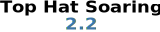
\includegraphics[angle=0,width=0.66\textwidth,keepaspectratio='true']{graphics/title.pdf}
    \end{center}
    \begin{center}
      \normalfont\huge\textsf{La Navigation Open Source}\par
    \end{center}
    \vskip 1cm
    \begin{center}
      \normalfont\huge\textsf{\@title}\par
    \end{center}
    \vskip 1cm
  \end{maxipage}

  \vfill
  \todo[nolist,size=\Large,inline]{Traduction en cours, v�rifiez qu'il n'y a pas de version plus r�cente avant d'imprimer.}

  \begin{flushright}
    \large \strut {
      \sf
      \today \\
      XCSoar version \version \\
      \xcsoarwebsite{} \\
    } 
    \par
  \end{flushright}
  \par
  \vfil
  \vfil
  \null
  \cleardoublepage
}

\DeclareUnicodeCharacter{00B0}{$^{\circ}$}

\begin{document}

%%%%%%%%%%%%%%%%%%%%%%
% Front page
\maketitle

 
%%%%%%%%%%%%%%%%%%%%%%
% Table of contents
\begingroup
\fontfamily{ptm}
\normalsize
\fontseries{c}\selectfont
\setlength{\parskip}{0.05\baselineskip}
\tableofcontents
\endgroup


%%%%%%%%%%%%%%%%%%%%%%
\chapter*{Preface}

\section*{Cuidado e Precauções}

\warning É DE RESPONSABILIDADE DO USUÁRIO QUE FAÇA A
UTILI\-ZAÇÃO DESTE SOFTWARE COM PRUDÊNCIA. ESTE
SOFTWARE TEM O OBJETIVO DE SER UTILIZADO SOMENTE
COMO AUXÍLIO À NAVEGAÇÃO E NÃO DEVE SER UTILIZADO
PARA NENHUM PROPÓSITO QUE NECESSITE MEDIÇÕES
PRECISAS DE DIREÇÃO, DISTÂNCIA, LOCALIZAÇÃO OU
TOPOGRAFIA. ESTE SOFTWARE NÃO DEVE SER UTILIZADO
COMO AUXÍLIO PARA DETERMINAR A PROXIMIDADE COM O
SOLO PARA NAVE\-GAÇÃO AÉREA. ESTE SOFTWARE NÃO DEVE
SER UTILIZADO COMO UM SISTEMA ANTI-COLISÃO AÉREA.



%%%%%%%%%%%%%%%%%%%%%%
\section*{Notas Legais}

\subsection*{Acordo de licença de Software}

Este software é lançado de acordo com a GNU - General Public License
Versão~2. Veja Anexo~\ref{cha:gnu-general-public} para o texto completo do acordo e notas de
garantia.

\subsection*{Responsabilidade Limitada}

Em nenhuma circunstância o XCSoar, ou seus responsáveis, acionistas,
diretores, empregados, afiliados, contratados, subsidiários ou
organizações proprietárias, serão imputados por qualquer incidente,
danos punitivos ou qualquer outro dano relativo ao uso deste produto.

\subsection*{Reivindicações}
Este produto e todos os arquivos que o acompanham, dados e materiais,
são distribuídos “no estado” em que se encontram, sem qualquer
garantia alguma, exceto o que está impresso ou escrito. Este produto
deve ser utilizado sob risco total do usuário. Todavia, foi tomado os
devidos cuidados durante seu desenvolvimento para eliminar defeitos
para ser um produto sem falhas. Nenhuma reivindicação pode ser legal
a respeito da confiabilidade ou aptidão do produto por nenhum
propósito particular. Os projetistas do XCSoar e seus contribuidores não
devem ser responsabilizados por erros internos ou danos, perda de dados
ou injúria pessoal com a conexão com o dispositivo, desempenho ou uso
deste material.


%%%%%%%%%%%%%%%%%%%%%%
\chapter{Introduction}\label{cha:introduction}
Ce document est le manuel d'utilistion de XCSoar, logiciel de navigation aérienne, open-source développé à l'origine pour les Poket PC. Le lecteur est sensé avoir de bonnes connaissances des fondamentaux de la théorie  du vol à voile et un minimum de pratique du vol sur la campagne.

Les mises à jour périodiques du logiciel peuvent rendre ce manuel périmé concernant certains points. Il est souhaitable de lire les notes de mise à jour du logiciel pour en connaitre les évolutions. Les mises à jour du logiciel et de la documentation sont disponibles sur 
\begin{quote}
\xcsoarwebsite{/download}
\end{quote}

\section{Organisation du manuel}

\todonum[inline]{Write about the manual crossref hinting icons and the yellow
colour. The Quickstart will be readable also without those links available} 
Ce manuel est structuré par grandes fonctionnalités du point de vue du pilote. La suite de ce chapitre parle du téléchargement, de l'installation et du lancement du logiciel sur les différentes plateformes matérielles supportées. Le chapitre ~\ref{cha:interface} décrit les concepts de l'interface utilisateur et donne une vue générale de l'affichage.

Le chapitre~\ref{cha:navigation} décrit en détail l'utilisation de la carte mobile et l'aide que peut apporter le logiciel de navigation. Le chapitre~\ref{cha:tasks} décrit comment les circuits sont définis et utilisés en vol. Il présente aussi les outils d'analyse permettant aux pilotes d'améliorer leurs performances. Le chapitre~\ref{cha:glide}  est consacré au calculateur de vol d'XCSoar et présente en détail les fonctionnalités qu'il offre. Il est important pour les pilotes de comprendre comment le calculateur effectue ses différents calculs.

Le chapitre~\ref{cha:atmosph} parle de l'interfaçage du calculateur avec des varios et autres instruments de mesure et comment ces données sont utilisées pour représenter différents modèles concernant entre autre le vent et la convection. Le chapitre~\ref{cha:airspace} parle de la gestion des espaces aériens et des alarmes dédiées ainsi que des alarmes du FLARM. Le chapitre~\ref{cha:avionics-airframe} présente l'intégration du calculateur avec le reste des systèmes utilisés dans l'environnement de vol ( terminaux permettant de communiquer avec le calculateur, switches divers) et des diagnostiques possibles.

La suite du document est constituée principalement de chapitres de référence. Le chapitre~\ref{cha:infobox} liste les différentes informations qui peuvent être affichées dans les "InfoBox" sur les côtés de la carte mobile. La configuration du logiciel est décrite dans le chapitre ~\ref{cha:configuration}. Le format des fichiers utilisés ainsi que la manière de les obtenir ou les créer et les éditer est décrit dans le chapitre~\ref{cha:data-files}.

Enfin, un bref historique et une explication du processus de développement de XCSoar sont présentés dans le chapitre ~\ref{cha:history-development}.

\section{Remarques}

\subsection*{Terminologie}
Un certain nombre de termes sont utilisés pour la description de matériel embarqués tels que Pocket PC, comprenant 'organiser', Portable Digital Assistant (PDA), et Personal Navigation Assistant (PNA). XCSoar est aussi disponible sur plateforme Altair(calculateur Triadis) qui est concrètement un instrument de navigation et plusieurs autres plateformes. Dans ce document ces termes sont utilisés indifféremment comme référence à un matériel supporté par XCSoar.

\subsection*{Copies d'écran}
Tout au long de ce manuel des copies d'écran de XCSoar sont présentées. Elles proviennent de différentes plateformes matériel et pas forcément de la même version d'XCSoar. Entre plateforme il peut y avoir des différences de résolution d'écran, de présentation générale, de police de caractères ce qui induit des différences entre la documentation et la visualisation sur l'appareil. La plupart des copies d'écran de ce manuel sont faites avec un affichage d'XCSoar en format paysage.

\section{Platformes}
\begin{description}
\item[Windows PC]
XCSoar fonctionne sur un PC sous Windows (XP, Vista, 7 versions 32 et 64 bits). Cette version est principalement utile pour la prise en main, l'entrainement à l'utilisation d'XCSoar, rejouer des fichiers IGC enregistrés ou utiliser XCSoar en mode simulation sur un PC non connecté à un GPS.
\item[Windows Mobile PDA/PNA]
XCSoar supporte les appareils utilisant Microsoft Pocket PC 2003 jusqu'à Windows Mobile 6. Windows Mobile 7 n'est pas supporté car Microsoft a décidé de ne pas maintenir les applications natives à partir de cette version.  
\item[Unix/Linux PC]
XCSoar peut tourner sous Unix en utilisant l'émulateur Wine. Une version native Unix existe à partir de la version 6.0 mais est toujours considérée comme expérimentale.     
\item[Périphériques Androïd] supporté à partir d'Androïd 1.6 et versions ultérieures.
\item[Altair] Le calculateur de vol Altair, de triadis engineering GmbH, dans lequel XCSoar est pré-installé. la version Altair PRO comporte un GS interne. 
\end{description}



\section{Support technique}

\subsection*{Dépannage}
XCSoar est développé par une petite équipe. Bien que nous soyons heureux de vous aider dans l'utilisation de notre logiciel, nous ne pouvons donner de cours sur l'utilisation des techniques modernes d'information!
Si vous avez des questions concernant XCSoar, consultez la FAQ en premier lieu. Si vous ne trouvez pas de réponse satisfaisante, envoyez un mail à la liste:
\begin{quote}
\href{mailto:xcsoar-user@lists.sourceforge.net}{xcsoar-user@lists.sourceforge.net}
\end{quote}

Les nouvelles questions seront ajoutées à la FAQ du site de XCSoar. 

Vous pouvez aussi vous inscrire à la liste de mails de XCSoar afin d'être averti des derniers développements du logiciel. Pour plus d'information voir sur notre site:
\begin{quote}
\xcsoarwebsite{/discover/mailinglist.html}
\end{quote}

Le fichier de "log" du démarrage du logiciel est \verb|xcsoar.log|. Il peut être envoyé aux développeurs d'XCSoar pour les aider à déterminer les causes de problèmes au lancement du logiciel.

Pour les utilisateurs d'Altair le fichier de log est transféré vers le répertoire `FromAltair' à l'aide d'AltairSync si un support de stockage USB est connecté et qu'Altair est déjà sous tension.

\subsection*{Mises à jour}
Il est souhaitable de visiter le site web de XCSoar pour vérifier si il n'y a pas de mise à jour disponible. La procédure d'installation décrite au chapitre~\ref{cha:installation} suivant peut être répétée pour la mise à jour du logiciel. Les fichiers de configurations et les données personnelles (cartes, points de virage,...) sont préservées lors des mises à jour et ré-installations.

Il est bien entendu recommandé de mettre à jour les données de navigation (cartes, espaces aériens) pouvant être modifiées par les autorités. Le fichier d'espace aérien mis à disposition sur le site de la FFVV est mis à jour environ une fois par mois au cours de la saison.

\subsection*{Mises à jour de XCSoar sur Altair}
La lise à jour du logiciel sur Altair implique de télécharger le dernier fichier {\tt XCSoarAltair-YYY-CRCXX.exe} et de le copier sur une clé USB ou une carte SD. Ensuite utiliser l'utilitaire AltairSync sur le terminal Altair pour terminer l'installation. Pour plus de détails, se référer au {\em Manuel d'utilisateur Altair}.

Les autres types de données ou programmes peuvent être installés sur Altair de la même façon.

\subsection*{Vos retours}
Comme tout programme élaboré, XCSoar peut comporter des bugs. Si vous en trouvez un, veuillez le remonter à l'équipe de développement en utilisant notre portail dédié à:
\begin{quote}
\xcsoarwebsite{/trac}
\end{quote}
ou en nous contactant par mail à:

\begin{quote}
\href{mailto:xcsoar-devel@lists.sourceforge.net}{xcsoar-devel@lists.sourceforge.net}
\end{quote}

\section{Entrainement}
Pour votre sécurité et celle des autres, les pilotes utilisant XCSoar doivent s'entrainer à l'utilisation du logiciel, au sol , afin de s'habituer à l'interface utilisateur et au différentes fonctionnalités qu'il offre, AVANT de l'utiliser en vol.

\subsection*{XCSoar sur un PC}
La version PC permet de se familiariser avec le logiciel, son interface utilisateur et ses fonctionnalités tout en étant confortablement installé à la maison, une bière à la main.... Tous les fichiers et les configurations de cette version sont identiques aux versions embarquées. Il est donc très facile de tester différentes configurations sur le PC avant de les mettre en pratique en vol.

La version PC peut être connectée à des instruments et fonctionner comme un calculateur en l'air. Exemples d'utilisation:

\begin{itemize}
\item Connecter un FLARM au PC pour utiliser XCSoar comme station au sol, pour afficher le traffic des planeurs équipées de FLARM.
\item Connecter un variomètre "intelligent"  comme le Vega pour tester le paramétrage du vario.
\end{itemize}

\subsection*{XCSoar avec un simulateur de vol}
Une bonne manière d'apprendre à se servir du logiciel est de connecter un Pocket PC à un PC sur lequel tourne un simulateur de vol qui peut envoyer des messages NMEA vers un port série. Condor et X-Plane le permettent par exemple.

Le gros avantage de s'entrainer ainsi est que XCSoar peut être utilisé en mode FLY. Ainsi, il se comporte exactement comme si vous voliez et vous pouvez avoir un très bon aperçu du fonctionnement de XCSoar quand vous utilisez le simulateur de vol. 

\section{XCSoar et la sécurité}
L'utilisation d'un calculateur tel que XCSoar en vol entraine certains risques: l'attention du pilote peut être diminuée de manière très significative, comme le temps passé à regarder en dehors du cockpit pour assurer la sécurité.

La philosophie guidant la conception et le développement de XCSoar est de réduire cette distraction en minimisant les interactions de l'utilisateur et en présentant les informations de façon claire et lisible d'un coup d'œil.

Les pilotes qui utilisent ce logiciel sont responsables de l'utilisation de XCSoar en sécurité. 
Pour bien utiliser XCSoar vous devez:
\begin{itemize}
\item Devenir familier avec l'interface graphique et avec vous entrainer au sol.
\item En vol, prendre l'habitude de regarder dehors autour de vous avant d'interagir avec le logiciel.
\item Configurer le logiciel pour profiter des fonctionnalités automatisées pour minimiser les interactions avec le logiciel. Si vous vous apercevez que vous faites mécaniquement des actions fréquentes, demandez-vous (ou à un autre utilisateur de XCSoar) si le logiciel ne peut pas être configuré pour le faire à votre place.
\end{itemize}


%%%%%%%%%%%%%%%%%%%%%%
\chapter{Instalação}\label{cha:installation}

\section{Para rodar o XCSoar}
Você precisará obter os seguintes itens:

\begin{itemize}
\itemsep0em
\item um dispositivo que rode o XCSoar
\item XCSoar
\item um receptor de GPS
\item um arquivo waypoint 
\item um arquivo de espaço aéreo (opcional)
\item um arquivo de mapa (opcional)
\end{itemize}

\section{! Antes de voar a primeira vez com o XCSoar !}

Depois de ter instalado com sucesso o XCSoar, assim que você ligar o software, XCSoar irá apresentar uma pré-configuração pronta para o uso.  Mas esteja atento, pois até aqui este novo brinquedo só irá lhe fornecer um mapa em movimento.  Não confie nos dados computados.  Você deve indicar para o XCSoar qual aeronave está voando.  Isto é feito especificando os dados da sua aeronave, como curva polar, peso e outros dados.  Todavia, é sempre uma boa idéia estudar o manual e se tornar familiar com o XCSoar em casa.

\section{Como conseguir o máximo do XCSoar}

Para se conseguir o benefício máximo do XCSoar, você deve fazer mais do que simplesmente instalar o software e fazer o download de alguns arquivos de dados.  Este algo mais inclui dados pessoais e da aeronave, como configuração e ajustes de algumas características.  Se você estiver disposto a obter tudo o que o XCSoar fornece, pode ser feito em um espaço razoavelmente curto de tempo.  Os passos necessários estão resumidos em uma checklist, fornecida no próximo capítulo.

Se você estiver planejando organizar um sistema com vários componentes internos, este manual irá lhe fornecer conselhos valiosos de como fazer os ajustes e configurações e como utilizá-los.

Se é um piloto com urgência, os autores sugerem que você utilize o Manual XCSoar-in-a-Flash através da checklist de passo-a-passo.  O manual resumido está disponível em: 
 \url{http://www.xcsoar.org/
discover/manual.html}.



\section{Checklist do XCSoar}

\subsection*{Faça o XCSoar}
\begin{itemize}
\item tenha o hardware e instale o XCSoar
\item tenha os arquivos de dados apropriados do seu local de vôo
\item configure o XCSoar para os arquivos de dados úteis
\item indique para o XCSoar a curva polar e peso
\item possibilite conectá-lo à instrumentos
\item finalize as configurações e se familiarize
\item monte o hardware
\item adicione os itens listados à sua checklist
\item faça o waypoint "Casa"
\end{itemize}

\subsection*{O procedimento de verificação pré-vôo inclui}
\begin{itemize}
\item ajuste da polar e peso
\item ajuste os parâmetros de vento e vôo (MC, Insetos, QNH)
\item se possível, execute uma prova válida.
\end{itemize}

\subsection*{O procedimento de ínício inclui}
\begin{itemize}
\item Verifique o vento e ajustes de vôo mais uma vez
\end{itemize}
\vspace{2em}

\subsection*{Voe, aprecie}
\vspace{4em}

\subsection*{Procedimento de verificação após o vôo}
\begin{itemize}
\item Baixe o registro de vôo do registrador e faça o upload para o Skylines e OLC.
\item Reuna os dados estatísticos do vôo.
\end{itemize}
\newpage




\section{Compatibilidade}

\subsection*{Dispositivos para rodar o XCSoar}

O XCSoar roda nas plataformas abaixo:

\begin{itemize}
\item PDAs com Pocket PC 2000, 2002, 2003 \\
  Examplo: iPaq 3800, iPaq 3900
\item PDAs com Windows Mobile \\
  Examplo: iPaq hx4700, Dell Axim x51v
\item PNAs com Windows CE 3.0 ou mais recente \\
  Exemplo: HP314, Mio400
\item Android mobile phones e tablets com Android 1.6 ou mais recente \\
  Exemplo: Dell Streak, Samsung Galaxy S II, HTC Desire HD,
  Motorola Xoom
\item eReader Kobo (experimental, Dez. 2013)
\item Triadis Altair
\item LX MiniMap
\item Windows 2000 ou mais recente
\item Linux
\item Mac OS X (desatualizado)
\end{itemize}

\subsection*{GPS, Registrador, Vario}

O XCSoar é compatível com qualquer GPS que emita dados NMEA.  A maioria dos dispositivos modernos de Android tem um receptor de GPS interno, mas por várias razões, é aconselhável conectar um ou mais dispositivos externos:

\begin{itemize}
\item um receptor especial de GPS tem maior ganho e fornece dados mais precisos para medições e cálculos
\item um indicador de velocidade do ar permite uma estimativa rápida sem que o piloto necessite realizar curvas
\item um variômetro melhora o assistente de termal
\item uma prova pode ser declarada a um registrador IGC e após o pouso, pode-se fazer o download do vôo. 
\item alguns variômetros permitem sincronismos com ajustes de MacCready e o XCSoar.
\item FLARM  (e mesmo a entrada ADS-B) fornece informações e posições de outros ao redor (e claro, FLARM fornece a detecção de colisão).
\end{itemize}

\subsection*{Dispositivos externos suportados e características}
\label{sec:supported-varios}

\newcommand{\y}[0]{{ $\surd$ }}
%{0.8\textwidth}
\noindent\makebox[\textwidth]{%
\begin{tabular}{l|ccc|cc|cc|c}
       \multicolumn{1}{r}{Suportado:} & \multicolumn{3}{c|}{-Caract.} & \multicolumn{5}{c}{-Fluxo Dados} \\
NMEA Device & 
  \begin{sideways} Declaração\end{sideways} & 
  \begin{sideways} Ctrl.Remoto\end{sideways} & 
  \begin{sideways} Download\end{sideways} &
  \begin{sideways} Velocidade ar\end{sideways} & 
  \begin{sideways} Vario\end{sideways} & 
  \begin{sideways} Baro. altitude\end{sideways} & 
  \begin{sideways} Vento\end{sideways} &
  \begin{sideways} G-Sensor\end{sideways} \\
\hline
%                    _Decl_Remo_Down_Airs_Vari_Baro_Wind_Gsen_
Borgelt B50          &    & \y &    & \y & \y & \y &    &    \\
CAI 302              & \y & \y & \y & \y & \y & \y & \y & \y \\
CAI GPS Nav          &    &    &    &    &    &    &    &    \\
Condor               &    &    &    & \y & \y & \y & \y &    \\
\hline
Digifly Leonardo     &    &    &    & \y & \y & \y & \y &    \\
EW Logger            & \y &    &    &    &    & \y &    &    \\
EW microRecorder     & \y &    &    &    &    & \y &    &    \\
FLARM                & \y &   & \y  &    &    & \y &    &    \\
\hline
%                    _Decl_Remo_Down_Airs_Vari_Baro_Wind_Gsen_
Flymaster F1         &    &    &    &    & \y & \y &    &    \\
Flytec 5030          &    &    &    & \y & \y &    &    &    \\
GTAltimeter          &    &    &    &    &(\y)& \y &    &    \\
ILEC SN10            &    &    &    &    & \y & \y & \y &    \\
\hline
IMI ERIXX            & \y &    & \y &    &    &    &    &    \\
LX20, Colibri        & \y &    & \y &    &    & \y &    &    \\
LXNAV Nano           & \y &    & \y &    &    &    &    &    \\
\hline
%                    _Decl_Remo_Down_Airs_Vari_Baro_Wind_Gsen_
LXNAV V7             &    & \y &    & \y & \y &    &    &    \\
PosiGraph            & \y &    &    &    &    & \y &    &    \\
Triadis Altair (pro) & \y &    &    &    &    & \y &    &    \\
Triadis Vega         &    & \y &    & \y & \y & \y &    & \y \\
\hline
Vaulter              &    & \y &    & \y & \y & \y & \y & \y \\
Volkslogger          & \y &    & \y &    &    & \y &    &    \\
Westerboer VW1150    &    & \y &    & \y & \y & \y &    &    \\
Zander / SDI         &    & \y &    & \y & \y & \y & \y &    \\

\end{tabular}}
\footnotetext{LX - Enquanto a maioria dos dispositivos com Windows CE têm porta serial, esta funcionalidade não está disponível nos dispositivos mais modernos com Android.  Estes podem ser usados com bluetooth ou placa IOIO para Android.  Para usar bluetooth, você precisa conectar o dispositivo externo a um adaptador serial, como o K6-Bt ou o Glidertools VFBT-1.}


\section{Instação do Software}

O software está disponível para download gratuito no site XCSoar    
~\xcsoarwebsite{}.  Esta seção descreve qual arquivo deve ser baixado e como instalar.

\subsection*{No Android}

Obtenha o XCSoar do mercado Android (GooglePlay) ou instale o aplicativo manualmente.  Copie os arquivos de dados para o cartão SD no diretório 
\verb|XCSoarData|.

\subsection*{No Kobo Mini}

O Kobo Mini é um dos mais baratos leitores de e-book.  Tem uma tela branca e preta com excelente leitura sob iluminação solar.  
Antes de você começar: faça uma cópia do cartão SD interno.  O instalador do XCSoar talvez interrompa seu funcionamento, mas você pode ter sempre como recuperar o Kobo se houver uma falha do software, mas somente se tiver um backup.
Para instalar o XCSoar, conecte o Kobo ao seu computador via USB. O Kobo mostra como um dispositivo de armazenamento no seu PC; abre e cria diretório chamado \texttt{.kobo} (note o ponto final antes do nome do diretório).  Baixe o arquivo \texttt{KoboRoot.tgz} do site do XCSoar neste diretório (\url{http://www.xcsoar.org/hardware/}). Desconecte o Kobo e reinicie-o (desligue completamente e religue).  Você verá a mensagem “Updating” e após alguns minutos, o Kobo mostra um menu que permite você carregar o XCSoar ou o software de leitura de e-book da Kobo.

Para copiar os arquivos de dados (mapas, waypoints), para o Kobo, rode o software original Kobo (“Nickel”) e conecte o Kobo ao seu micro novamente.  Copie os arquivos na raiz do diretório  \texttt{XCSoarData}.

Em outra alternativa, os arquivos de dados podem ser baixados via gerenciador de arquivos XCSoar, depois de ter conectado em uma rede Wi-Fi e com o XCSoar rodando.

\subsubsection{Pirateando o Kobo}

Depois de instalar o XCSoar no Kobo, o novo comando de reinicio executa o arquivo \texttt{XCSoarData/kobo/init.sh}.  Se você sabe o que está fazendo, você pode usar esse comando no momento do reinicio para executar outras ações: \texttt{inetd} (para acesso \texttt{telnet}
).

Quando você roda o \texttt{Nickel} (the original e-book firmware), o novo script também verifica outro script chamado \texttt{XCSoarData/kobo/init\_nickel.sh} e o executa.  Novamente, se tem conhecimento, pode usar este script para executar ações antes da inicialização do \texttt{Nickel} se completar, por exemplo, configurando o reconhecimento de seu variômetro externo (para desligar, alterar o volume, etc...).

\subsection*{Em um PDA (Windows Mobile, PocketPC)}

Escolha um dos sistemas:

\begin{description}
\item[\texttt{PPC2000}] Pocket PC 2000/2002, Windows CE 3.0
\item[\texttt{PPC2003}] Pocket PC 2003, Windows CE 4.0
\item[\texttt{WM5}] Windows Mobile 5 iu mais recente
\item[\texttt{WM5X}] Windows Mobile 5 ou mais recente com  XScale CPU ou melhor (e.g. hx4700)
\end{description}

Baixe o arquivo \verb|XCSoar.exe| para um cartão SD.  Você pode  rodar com o explorador de arquivos.
\sketch{figures/XCS_Today.png}
Outro método de instalar o XCSoar em um PDA é o arquivo CAB.  Baixe no cartão SD.  Use o explorador de arquivos para instalar.  Após a instalação, os ícones “FLY” e “SIM” estarão visíveis na tela atual.


\subsection*{Para PNA (Windows CE)}

Baixe o arquivo de programa \verb|XCSoar.exe| (alvo ``WM5'') para um cartão SD.  Pode rodar com o explorador de arquivos.

\subsection*{Para a Windows PC}

Baixe o arquivo de programa \verb|XCSoar.exe| (alvo ``PC'') para o seu disco rígido.

\subsection*{No Unix/Linux}

O arquivo baixado é \verb|xcsoar_XXX.deb|, onde \verb|XXX| a versão e plataforma são \verb|xcsoar_6.0.4_i386.deb|.
Há um pacote Debian e pode ser instalado usando
\begin{center}
\verb|sudo dpkg -i xcsoar_XXX.deb|.
\end{center}
Use \verb|dpkg-query -L xcsoar| para ver onde os arquivos foram instalados.  Dados adicionais devem ser alocados no \verb|~/.xcsoar|.
Se \verb|~/.xcsoar| não existir, será criado na primeira vez que o \verb|xcsoar| rodar.

\subsection*{No Raspberry Pi e Cubieboard}

Instale o pacote Debian como descrito acima.  Porém, ao contrário do Linux comum, o XCSoar não irá usar o X11.  Ao invés disso, rodará em tela cheia no console Lixus.

O XCSoar necessita acessar seus dispositivos de entrada
(\texttt{/dev/input/event*}).  Por padrão, somente acesso garantido ao \texttt{root}.  Para reescrever,  \texttt{udev}, crie uma regra de configuração \texttt{/etc/udev/rules.d/99-input.rules}:

\begin{verbatim*}
KERNEL=="event*", NAME="input/%k", MODE="660", GROUP="input"
\end{verbatim*}

Crie o grupo \texttt{input} e seja membro:

\begin{verbatim*}
groupadd input
adduser pi input
\end{verbatim*}

\section{Arquivo de Dados}\label{sec:data files}

Seja capaz de usar as características avançadas dos arquivos de dados do XCSoar, como terrenos, topografia, espaço aéreo, waypoints, etc.  
Estes arquivos que podem ser usados com o XCSoar são descritos no Capítulo
\ref{cha:data-files}.

Todos os dados devem ser copiados no diretório 
\texttt{XCSoarData}.  Este diretório deve estar em um local específico que o XCSoar sabia onde procurar por arquivos de dados.

\begin{description}
\item[Windows PC]
\texttt{XCSoarData} no seu diretório pessoal (``\texttt{My
Documents}'')
\item[Windows Mobile PDA/PNA]
Se houver um diretório chamado \texttt{XCSoarData} no mesmo diretórioi que \texttt{XCSoar.exe}, então este não será usado.
\texttt{XCSoarData} está no cartão SD.  Se não houver cartão SD, o XCSoar irá procurar pelo diretório nos \texttt{My Documents}.
\item[Unix/Linux]
O diretório é chamado \verb|.xcsoar| no diretório raiz.
\item[Dispositivos Android]
\texttt{XCSoarData} está no cartão SD.
\item[Altair]
se o diretório XCSoarData estiver em um drive USB, este será usado, ao contrário, o armazenamento interno será usado.
\end{description}


O XCSoar irá gerar um número adicional de arquivos enquanto roda.  Estes serão alocados no diretório  \texttt{XCSoarData} (Windows PC, 
Windows e dispositivos Android móveis), ou no diretório \texttt{.xcsoar} para (Unix/Linux
PC).  Na primeira vez que rodar, o XCSoar irá criar e manter arquivos
\texttt{Default.tsk} (Default Task),  
\texttt{default.prf} 
(ajustes das configurações),
\texttt{xcsoar.log}, 
mais três diretórios: \texttt{cache},
\texttt{config} e \texttt{logs}.  Arquivos adicionais e registros de vôo podem ser criados e/ou modificados enquanto o XCSoar roda (\texttt{*.tsk}) .


\section{Rodando o XCSoar}
%\subsection*{Fly and simulator modes}

Dois modos são permitidos dentro do XCSoar: 
\begin{description}
\item[FLY]este modo é usado quando está voando.  O simulador é desabilitado e as comunicações seriais estão ativas.
\item[SIM] :  este modo roda o XCSoar em simulação, não há comunicação serial disponível.
\end{description}

\subsection*{Versão Altair}
O XCSoar inicia automaticamente quando o Altair é ligado.  O botão PWR/ESC tem múltiplas funções:
\begin{description}
\item[Ligar]  aperte e segure PWR/ESC por um segundo.  O LED no botão irá acender e o XCSoar irá iniciar em seguida.
\item[Desligar] aperte e segure PWR/ESC por 3 segundos.  O Altair irá desligar.
\item[Escape] apertando PWR/ESC rapidamente, atua como uma tecla ESC, usada geralmente para fechar páginas de diálogo ou cancelar funções.

\end{description}

A versão do XCSoar para Altair não inclui modo de simulação.

\subsection*{XCSoar versão PC}

O programa pode ser aberto na janela do explorador, encontrando qual o diretório que contém o XCSoar.exe executável, e clique duas vezes no arquivo de programa.
Estas opções do programa permitem que se defina a orientação da tela:

\begin{description}
\item[-retrato] :   A tela tem largura de 480 e altura de 640 pixels.
\item[-quadrado] a tela tem 480 x 480 pixels.
\item[-paisagem] :   a tela tem 640 pixels de largura e 480 pixels de altura.  Esta é a configuração mais comum.  Se você não especificar este parâmetro, esta visualização será carregada automaticamente.
\item[-pequena] desenha a tela com metade do tamanho normal.  É útil para usar o XCSoar em conjunto com simuladores de vôo (ex. Condor).
\end{description}
Para alterar a orientação da tela, é conveniente criar atalhos para o programa.  Clique no ícone do atalho e no campo “Alvo”, adicione uma das opções escolhidas acima.

\subsection*{Versão XCSoar Unix/Linux PC}
Rode o \verb|xcsoar| de uma linha de comando ou crie um atalho no desktop.  
Somente o modo de paisagem é permitido agora.


\subsection*{Carregando arquivos de dados}\label{sec:loaddatafiles}
A primeira vez que o XCSoar é iniciado, não carrega automaticamente os arquivos de dados que você descarregou no diretório \verb|XCSoarData|.  
Para mostrar quais dados deverão ser carregados, clique no mapa (a maior parte da tela, com o glider branco no centro), escolha menu \bmenug{Config 2}, e então clique 
\bmenug{Sistema}.  A tela de configurações deverá mostrar:
\sketch{figures/config-basic.png}
já na primeira página permite que você escolha os arquivos de mapa, waypoints, e espaço aéreo, clicando nas caixas de texto.  Muitas outras características do XCSoar devem ser configuradas aqui.  Estão descritas no Capítulo 
\ref{cha:configuration}.
Uma vez completa, XCSoar recarrega estes arquivos; de agora em diante estes arquivos de dados serão automaticamente carregados.

\subsection*{Início e perfis de usuários}\label{sec:profiles}
Quando o XCSoar inicia, ele verifica por perfis existentes.  Se houverem múltiplos perfis, será mostrada uma pequena janela perguntando qual perfil deseja carregar.  Para prosseguir, escolha o perfil apropriado e clique ENTER.  Se não houver escolha do perfil, serão carregados os ajustes da última seção.  Os perfis podem ser utilizados para os seguintes casos:
\begin{itemize}
\item Pilotos diferentes
\item Competição versus vôo casual
\item Voando em locais diferentes
\item Diferentes aeronaves (com diferentes polares)
\end{itemize}
Os perfis também devem ser armazenadores e preservadores de certas configurações.  Virtualmente, cada ajuste do XCSoar é arquivado em um perfil com extensão \texttt{.prf}. Uma vez feliz com seus ajustes, faça duas cópias de seu arquivo de perfil.  Uma cópia com a extensão \texttt{.prf}, será carregada no início e reflete todas as alterações feitas enquanto o XCSoar está rodando; o arquivo \texttt{.bak} preservará os ajustes e configurações que você julga importante e que deve manter.

Um exemplo de como você deve criar os arquivos são:
\begin{itemize}
\item \texttt{buddiesinArcus.prf}
\item \texttt{buddiesinArcus.bak}
\item \texttt{willyboyinPrymuswonderland.prf}
\item \texttt{willyboyinPrymuswonderland.bak}
\end{itemize}

\subsection*{Modo SIM}
O XCSoar vem com uma interface simples permitindo a simulação de vôo.  Dependendo da plataforma (hardware), há diferentes métodos para alterar valores de bússola, velocidade, e altura.  A simulação tem por finalidade sua primeira familiarização com o XCSoar.  Se você gosta da idéia de simular um vôo mais realístico em casa, você deve adquirir um simulador de vôo “real” para ser conectado com o XCSoar.

Na tela de mapa, clicando ou tocando o símbolo do planador na tela de toque ou mouse e arrastando, faz o planador se mover na direção do arrasto, a velocidade é proporcional à distância do arrasto.

Com os botões, a velocidade da aeronave, altitude e direção podem ser alteradas usando as Infoboxes.  As informações a seguir podem não estar disponíveis em todas as plataformas de hardware, mas em todas as plataformas que o XCSoar suporta, é possível se configurar uma série de entradas para simulação.

Clicando em uma Infobox, você seleciona um valor para ser alterado por botões ou menus.
A altitude da aeronave pode ser definida selecionando a infobox GPS \bmenuw{Alt GPS}, e clicando acima ou abaixo na tela de toque.  A velocidade do ar pode se ajustada em \bmenuw{V Gnd}, clicando acima ou abaixo na tela de toque.  A trilha da aeronave pode ser ajustada selecionando a infobox \bmenuw{Trilha}, e clicando nos botões acima e abaixo.

Com ambos \bmenuw{Alt GPS} ou \bmenuw{V Gnd}
selecionados, a direção da aeronave pode ser alterada usando as teclas direita/esquerda.
Outros controles, botões e menus funcionam da mesma forma no modo FLY.


\subsection*{Tela de início}
Quando o XCSoar inicia, desliga ou carrega arquivos grandes, como espaço aéreos, waypoints, terrenos, etc, é mostrada uma tela de progresso enquanto os dados estão sendo carregados.  Esta tela tem uma barra de progresso que indica a atividade de carregamento e uma curta linha de texto é mostrada com a ação que está sendo executada.

Esta tela também mostra a versão do software.

\subsection*{Saindo do programa}
Para versões de PDA e PC, o XCSoar é desligado pelo menu que  pode ser aberto dando um duplo clique no mapa ou nas Infoboxes.
\begin{quote}
\bmenug{SAIR}
\end{quote}

Para versões para PC, o XCSoar pode ser desligado no ícone de fechamento da janela do o XCSoar.
Para Altair, o XCSoar pode ser desligado segurando o botão PWR por dois segundos ou mais. 


%%%%%%%%%%%%%%%%%%%%%%
\chapter{User Interface}\label{cha:interface}
\begin{figure}[h]
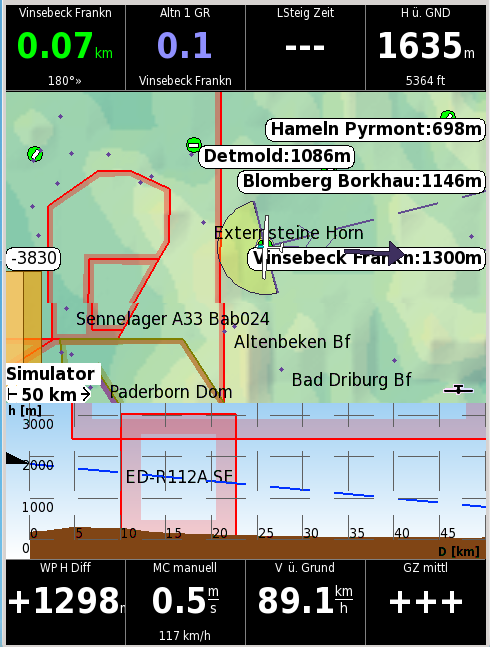
\includegraphics[angle=0,width=\linewidth,keepaspectratio='true']{figures/plain.png}
\caption{Typical XCSoar main screen layout}
\end{figure}

This chapter describes the fundamental user interface concepts used by 
XCSoar, and is intended as an overview. The \emph{main screen} covers much of 
the information needed during normal flight.  Typically, the main screen is 
composed of the moving map and infoboxes. For several reasons - not being the 
scope of an introduction - you have a choice of using several main screens 
in-flight, named \emph{screen pages}.

Screen pages are easily accessed by a horizontal swipe gesture just like 
turning pages of a book or button push, depending on the hardware you use. 
With screen pages you are enabled to compose several main screens to be used 
advantageously in different situations in-flight. Simply speaking, you are 
enabled to use appropriate information in different \emph{use cases}, to be 
accessed quite simply and fast. 

Whenever actual situations are worthy of grabbing the pilot's attention, an 
\emph{overlay} is put in front of the main screen. This happens especially 
when urgent reaction by the pilot is required as are the situation of a 
possible collision or an entering of a restricted airspace expected to happen
soon.

Evidently, menu buttons and menu screens are overlays too, and there are many 
more. As a result, the elements put on each other form a display stack with 
the main screen representing the base of it. More detailed descriptions are 
given in following chapters.



\section{Display elements}
\subsection*{Main screen and screen pages}
Every screen page out of XCSoar's screen pages' ensemble is composed of several 
parts:
\begin{description}
\item[Main area] The bulk of the screen typically is dedicated to the GPS moving 
map display. Various symbols relating to glide computer information are overlaid 
the map area. Icons and text may appear along the lower edge of the screen
to indicate status of connected devices, flight modes etc.
Following the development process of XCSoar there is an increasing number of 
items that may be chosen for display in the main area, which are gauges 
Flarm Radar, Thermal Assistant, and Horizon (as is with Version 6.7.2, 
Dec. 2013).
\item[InfoBoxes] A grid of data values is displayed usually either along
the top and bottom of the screen (portrait display) or to the right of the
screen (landscape display).  These so-called InfoBoxes display data from the
GPS and other input devices as well as data calculated by XCSoar. Further, 
Infoboxes can display even gauges and certain graphs.
\item[Bottom area] At the screen's bottom, XCSoar is able to draw a cross 
section of terrain and airspaces in direction of your heading. (There might be 
more to come after Dec. 2013)
\end{description}

\subsection*{Overlays}
\begin{description}
\item[Gauges]  Gauges provide instrumentation displays. All gauges are optional
and some may only have meaningful information displayed when XCSoar is
connected to a supported instrument.
A gauge overlay is either permanently drawn or is invoked by several 
conditions.  E.g. the thermal assistant is shown, when XCSoar enters circling 
mode. The Flarm radar is invoked, whenever a probable collision is detected. 
Permanently overlayed gauges are the final glide bar as well as the vario bar 
amongst others.
\item[Button labels and menus] Hardware buttons on the device running XCSoar
can be used to bring up and navigate smaller on-screen menus that are
typically laid out such that menu items can be selected by pressing the
button adjacent to the item.  If the device has a touch screen, the menu
items can be selected by touching them.  These buttons are drawn in black
text on a grey background.
\item[Status messages] Text is displayed over the screen in status message
boxes.  This text is used to present detailed information to the pilot when
certain events occur.
\item[Dialogue windows] Larger dialogue windows, usually containing graphics and
buttons, are used to present detailed data to the pilot regarding waypoint
details, statistics and analysis etc.
\item[Main menu] The main menu is accessible by double tapping the map area or
InfoBoxes as well as through gesture. If the menu buttons are not pressed after
\gesturespec{du} a specified time, they disappear again so as to not obscure 
the map area.
\end{description}

\subsection*{Classic vario gauge}
As said above, gauges might be displayed in different ways, either as an 
infobox, overlay, or even in the main area. The traditional variometer gauge is 
different. This needle-style gauge is invoked permanently by choosing an infobox 
layout including the variometer on the right side of the other infoboxes. 

\section{Interaction}
There are several ways to interact with XCSoar:
\begin{itemize}
\item Touching certain map elements
\item Touching InfoBoxes and on-screen menu buttons
\item `Gesturing', by e.g. drawing a dash from the left to the right
  on the screen (see Section \ref{sec:gestures} below).
\item `Dragging' the screen (touching the screen and moving before releasing).
\item Pressing application buttons on the device.
\item Pressing the cursor keys on the device.
\item Pressing keys or switches on an instrument connected to XCSoar.
\end{itemize}
Depending on the particular hardware used with XCSoar, not all of these methods
of interaction are possible and there may be different numbers or assignments
of buttons.

For the PC version of XCSoar, clicking the mouse over an item is equivalent to
touching it.

Since the Altair does not have a touch screen, all user interaction is performed
via physical buttons, switches or other external interface devices if connected.

\section{The main button menu}
The button menu is a set of buttons drawn on the screen and activated by touch
or hardware button presses.  Using buttons and the button menu is the primary
way the user interacts with XCSoar.

\subsection*{Interface basics}
The menu is organised into four different groups of functions, usually in
the form of a hierarchy.  The specific menu layout depends on the
hardware button configurations and platform, and may also be customised by the
user.

XCSoar can also accept input from external keyboards, game-pads, joysticks,
stick grip switches etc. A wide variety of functions can be assigned to these
inputs.
\sketch{figures/buttonmenu.png}

For Altair, there are four major menus, activated by pressing one of
the vertical strip of hardware buttons on the left of the display.
When a menu is activated, a strip of on-screen buttons appear along the 
bottom of the display.  Pressing the particular menu button again will
cycle through several pages of items.  Pressing the corresponding
horizontal button will activate that item.  At the last page, pressing
the menu button again will turn that menu off and the horizontal strip
of on-screen buttons disappear.  

On the PC version, these mode buttons are activated by the
1, 2, 3 and 4 keys.  The 6, 7, 8, 9 and 0 keys correspond to the horizontal
strip of buttons.

On the PDA version, the mode buttons are activated by the keys to the
side of the joystick/rocker button.

If the user doesn't interact with the computer for some time, the
menu will close automatically.  This menu time-out is configurable.
The escape key on PC, or the PWR/ESC button on Altair, can
also be used to close the current menu.

Menu buttons appear greyed out if the corresponding function is not available. 
For example, the ``Waypoint list'' function will appear grey if there are no waypoints loaded.

Several menu button labels have dynamic text based on context, in
order to make it clearer as to what happens when the button is
pressed.  The convention is used that a button's label describes what
will happen when the button is pressed.  For example, if the button
says \bmenug{MC Auto}, then pressing the button will turn on `Auto
MacCready', and the button label will then change to \bmenug{MC Manual}. 
In the menu list described below, generic labels are used.

\subsection*{Menu function groups}
This section describes the default layout of the menu system on all
platforms.  The functions performed by each button are explained more
fully in following chapters.

The primary menu buttons are activated by each of the vertical strip of buttons
on Altair, from top to bottom:
\begin{jspecs}
\item[\bmenug{Nav}] Actions for navigation control, primarily cross-country
gliding tasks.
\item[\bmenug{Display}] Actions to control the display.
\item[\bmenug{Config}] Configuration of XCSoar, connected devices, and in-flight
settings.
\item[\bmenug{Info}] Activates various informational dialogue windows.
\end{jspecs}

For the PC version, the keys 1, 2, 3 and 4 activate the 
corresponding menu.  The following menu item list has on the left side of most 
of the menu buttons links to the respective section. Follow them to get to all 
related details.

\section{Menu item overview}

\subsection*{Navigation menu}
\noindent\makebox[\textwidth]{%

\begin{tabularx}{1.44\textwidth}{c|ccccc}
\bmenus{Nav 1/2}
 & \bmenus{Task}
 & \bmenut{Previous}{Turnpoint}
 & \bmenut{Next}{Turnpoint}
 & \bmenut{Waypoint}{List}
 & \bmenus{Alternates} \\
see
 & \ref{cha:tasks}
 & \ref{sec:advanc-rest-tasks}
 & \ref{sec:advanc-rest-tasks}
 & \ref{sec:waypoint-selector-dialog}
 & \ref{sec:alternates} \\ \\
\bmenus{Nav 2/2}
 & \bmenut{Task}{Abort}
 & \bmenut{Mark}{Drop}
 & \bmenus{Target}
 & {}
 & {} \\
see
 & \ref{sec:taskabort}
 & \ref{sec:markers}
 & \ref{sec:waypointdetails}
\end{tabularx}}

You should not start using XCSoar without knowing about the `Alternates' feature. 
Any `Task' related item in the navigation menu is used for planned cross 
country flight and certainly the second step.

\subsection*{Display menu}
\noindent\makebox[\textwidth]{%

\begin{tabularx}{1.44\textwidth}{c|ccccc}
\bmenus{Display 1/2}
 & \bmenut{Zoom}{In}
 & \bmenut{Zoom}{Out}
 & \bmenut{Zoom}{Auto}
 & \bmenut{Info}{Cruise/...}
 & \bmenut{Pan}{On} \\
see
 & \ref{sec:zooming}
 & \ref{sec:zooming}
 & \ref{sec:zooming}
 & \ref{sec:screenpages}
 & \ref{sec:panning} \\ \\
\bmenus{Display 2/2}
 & \bmenut{Labels}{All/...}
 & \bmenut{Trail}{Full/...}
 & \bmenut{Terrain}{On/Off}
 & \bmenut{Topo.}{On/Off}
 & \bmenut{Airspace}{On/Off} \\
see
 & \ref{sec:maplabels}
 & \ref{sec:trail}
 & \ref{sec:terrain_topo}
 & \ref{sec:terrain_topo}
 & \ref{sec:terrain_topo}
\end{tabularx}}

Most of the display menu items are available on gestures, or special key 
short-cuts of your device. Once you are familiar with XCSoar you probably 
will use those menu items less frequently.

\subsection*{Configuration menu}
\noindent\makebox[\textwidth]{%

\begin{tabularx}{1.44\textwidth}{c|ccccc}
\bmenus{Config 1/3}
 & \bmenut{MacCready}{$+$}
 & \bmenut{MacCready}{$-$}
 & \bmenut{MacCready}{Auto}
 & \bmenus{Flight}
 & \bmenus{Wind} \\
see
 & \ref{sec:stf}
 & \ref{sec:stf}
 & \ref{sec:auto-maccready}
 & \ref{sec:flight-setup}
 & \ref{sec:wind-setup} \\ \\
\bmenus{Config 2/3} 
 & \bmenus{System}
 & \bmenus{Plane}
 & \bmenus{Devices}
 & \bmenut{File}{Manager}
 & \bmenus{Replay} \\
see
 & \ref{cha:configuration}
 & \ref{sec:glidepolar}
 & \ref{conf:comdevices}
 & {}
 & \ref{sec:logger-replay} \\ \\
\bmenus{Config 3/3} 
 & \bmenut{Logger}{Start}
 & \bmenus{Raw Logger}
 & \bmenus{Airspace}
 & \bmenus{Vega} \\
 & \bmenus{Profiles} \\
see
 & \ref{sec:logger}
 & \ref{sec:raw-logger}
 & \ref{sec:airspace-filter}
 & {}
 & {}
\end{tabularx}}

The configuration menu is typically part of the ground interaction with 
XCSoar. You are not expected to spend much time in-flight with tweaking 
the configuration, except you manually adjust wind or MacCready settings. 
The `Vega' item gives control over the  Vega intelligent variometer. This 
comprises a sub-menu.


\subsection*{Information menu}
\noindent\makebox[\textwidth]{%

\begin{tabularx}{1.44\textwidth}{c|ccccc}
\bmenus{Info 1/3}
 & \bmenut{FLARM}{Radar}
 & \bmenut{METAR}{TAF}
 & \bmenut{What's}{here?}
 & \bmenut{Check}{list}
 & \bmenus{Analysis} \\
see
 & \ref{sec:flarm-traffic}
 & \ref{sec:metar-taf}
 & {}
 & \ref{sec:checklist}
 & \ref{sec:analysis-climb} \\ \\
\bmenus{Info 2/3}
 & \bmenus{Status}
 & \bmenus{Weather}
 & \bmenut{Team}{Code}
 & \bmenut{FLARM}{Details}
 & \bmenut{Thermal}{Assistant} \\
see
 & \ref{sec:flight-status}
 & \ref{sec:weather-forecast}
 & \ref{sec:team-flying}
 & {}
 & \ref{sec:thermal-assistant} \\ \\
\bmenus{Info 3/3}
 & \bmenus{Credits}
 & \bmenus{Airspaces}
 & \bmenut{Message}{Repeat}
 & {}
 & {} \\
see
 & \ref{sec:credits}
 & 
 & 
 & 
 &
\end{tabularx}}

The information menu is always a good address, when not only a clue on 
how to set MacCready is requested, but rather more elaborate help on a 
larger scope tactical decision on your flight is requested.


\subsection*{The Vega variometer sub-menu of the configuration menu}
\noindent\makebox[\textwidth]{%

\begin{tabularx}{1.44\textwidth}{c|ccccc}
\bmenus{Vega 1}
 & \bmenut{Airframe}{Switches}
 & \bmenut{Setup}{Audio}
 & \bmenut{Manual}{Demo}
 & \bmenut{Setup}{Stall}
 & \bmenus{Accel} \\ \\
\bmenus{Vega 2}
 & \bmenut{ASI}{Zero}
 & \bmenut{Accel}{Zero}
 & \bmenus{Store}
 & \bmenut{Cruise}{Demo}
 & \bmenut{Climb}{Demo}
\end{tabularx}}

The functions in this sub-menu require the Vega intelligent variometer. 
The menu can only be accessed if `Vega' is selected as the connected device.

\subsection*{The pan mode sub-menu of the Display menu}

\noindent\makebox[\textwidth]{%

\begin{tabularx}{1.44\textwidth}{c|ccccc}
\bmenus{Pan}
 & \bmenut{Pan}{Off}
 & \bmenut{Zoom}{in}
 & \bmenut{Zoom}{out}
 & \bmenut{What's}{here?}
 & {} \\
see
 & \ref{sec:panning}
 & {}
 & {}
 & {}
 & {}
\end{tabularx}}

This sub-menu unfortunately overlays the full-screen map view of the pan mode.
 It's functions are quite evident, although the menu could be replaced by multi-touch
 technology or knobs (like on Altair). Besides the essential `exit pan mode'
 function the `What's here?' button offers brilliant access to the variety of
 information of the map.

\section{Default menu buttons}

When no menu is active, (so-called default mode), the horizontal row
of buttons in Altair perform the following functions (from left to right):

\begin{center}
\begin{tabular}{c c c c c c}
 PC: & 6 & 7 & 8 & 9 & 0 \\
 Altair: & F5 & F6 & F7 & F8 & F9 \\
& \bmenus{Flight} & \bmenut{Task}{Manager} & {} & \bmenus{Target} & \bmenut{Drop}{Mark} \\
\end{tabular}	
\end{center}

Pressing ESC on Altair displays labels for these default menu buttons.

For all other versions in the default mode, the cursor keys perform
the following functions:
\begin{jspecs}
\item[Up key] Zoom in
\item[Down key] Zoom out
\item[Left key] Drop marker
\item[Right key] Toggle through normal/aux. InfoBoxes and full-screen
\item[Enter] Clear status message or suppress FLARM gauge if open and no warning
active
\end{jspecs}

For the Altair version in the default mode, the rotary knob performs
the following functions:
\begin{jspecs}
\item[Outer knob counter-clockwise] Zoom in
\item[Outer knob clockwise] Zoom out
\item[Inner knob counter-clockwise] (No function assigned)
\item[Outer knob clockwise] (No function assigned)
\item[Knob button press] Clear status message or acknowledge airspace warning
\end{jspecs}

In dialogue forms, the rotary knob in Altair performs the role of the cursor and
enter keys:
\begin{jspecs}
\item[Outer knob counter-clockwise] Up cursor
\item[Outer knob clockwise] Down cursor
\item[Inner knob counter-clockwise] Left cursor
\item[Inner knob clockwise] Right cursor
\item[Knob button press] Enter key
\end{jspecs}

For Altair, the buttons along the edge of the display can be used as
alternate ways of navigating in dialogues.  The F4 key (directly above
the rotary knob) can be used as an alternate ENTER key (instead of
pressing the rotary knob) in dialogues.  The F6 and F7 keys (directly to
the right of the rotary knob) can be used to select the next or
previous page in multi-page dialogues.

\subsection*{Dynamic menu labels}
Certain menu items have dynamic labels to make it clearer what happens when the
menu item is selected.  Furthermore, items that are not available are greyed
out to indicate that selecting the menu item will not do anything.

The convention used for dynamic menu labels is for the labels to display the
action that will be performed once the menu item is selected. For example 
``Lights On'' will turn the lights on, and the menu will be updated to display
``Lights Off'', which would then if pressed turn the lights off. This
convention is used throughout XCSoar.

A selection of key dynamic menu items is presented below:
\begin{description}
\item[\bmenug{Next Turnpoint}]  
  Greyed out if the task is cleared, or if the active turnpoint is the
  finish. If the currently active turnpoint is the turnpoint prior to the 
  finish, this displays  ``Waypoint finish''.
\item[\bmenug{Previous Turnpoint}]  
  Greyed out if the task is cleared, or if the active turnpoint is the
  start and there are no multiple start points.  If there are multiple
  start points and the active turnpoint is the start, then this
  displays ``Cycle start'' to allow selection between the various
  start points.  If the active turnpoint is the first turnpoint after 
  the start, this displays ``Waypoint Start''.
\item[\bmenug{Labels All}]  
  This will turn on all labels available on the map. There are more options to 
  only show a reduced set of labels like ``Labels Task'', thus not cluttering the 
  screen too much.
\item[\bmenug{Target}]  
  Greyed out if the task is cleared or in task abort.
\end{description}


\section{InfoBoxes and screen pages}\label{sec:infoboxandpages}

The information displayed in the InfoBox fields can be selected from a
wide variety of options (listed in Chapter~\ref{cha:infobox}). These
fields can also be used to change for example the MacCready setting.

The specific number and layout of the InfoBox grid depends on the
screen orientation and the device's display size.  

For a 320x240 display
Pocket PC in portrait mode, there are four InfoBoxes above and four
InfoBoxes below the map display.  
\sketch{figures/infoboxes.png}

A typical landscape layout has 9 InfoBoxes and the variometer gauge 
to the right of the map display. 
For larger displays up to 24 InfoBoxes may be displayed simultaneously.  

In order to gain clarity, the less infoboxes you choose to be displayed at once, 
the faster your reading will be. On the other hand, there are much too many 
InfoBox options a pilot would hardly reject. The number of possible InfoBox 
options already exceeded one hundred. That is why XCSoar offers two ways of 
managing even more options than Info\emph{boxes} count.

Depending on your flight's state, whether you are circling or cruising, you can 
let XCSoar change the content of each single InfoBox. As an example you might 
change the display of the actual average climb whilst circling to speed to fly 
when cruising. The switch is derived automatically by entering different 
\emph{flight modes} (see section \ref{sec:flightmodes}) executing a switch to 
another \emph{InfoBox set}.

Further, you can use screen pages to change InfoBox content manually, by 
assigning different Infobox sets to different pages (see following section).

To gain access to automatic switching InfoBoxes dependent on the flight mode, 
just let XCSoar run with it's pre-configured setup from installation. To set up 
your personal version of Infoboxes go through the following procedure.
\begin{description}
\item[InfoBox geometry] Choose a basic Infobox geometry or layout.  This basic 
layout is maintained through any changes in-flight, affecting InfoBox content 
only.\config{interface-appearance}
\item[Choose Infobox set "Auto"] Configure at least one screen page with the 
choice of Infoboxes "Auto". As can be seen on the corresponding configuration 
screen, there are more screen pages pre-defined. \config{screenpages}  These 
others are not needed to gain automatic switches by flight mode. They are for \emph{manually} turning through the screens defined by pages. 
\item[Define InfoBox sets] Put together the Infobox content you want to be 
displayed in three Infobox sets called "Circling", "Cruise", and "FinalGlide" 
respectively.\config{infobox_sets}
\end{description}  


\subsection*{Screen pages with different InfoBox sets}\label{sec:screenpages}

XCSoar allows the pilot to define various sets of InfoBoxes that are 
appropriate for "normal" states of flight.  Assuming circling, 
cruising, or final glide as normal, XCSoar can switch corresponding Infobox 
sets automatically. Perfectly done.

As you might imagine, there are countless cases, you wished you had another 
ensemble of information displayed at once.  For all of these more or less 
special situations you can define up to eight screen pages, reflecting the 
actual \emph{use case}. Just to draw a brief sketch of the possibilities 
introduced by the concept of screen pages, a few use cases are given. 
\label{par:use_case}
\begin{description}
\item[Familiarisation] Especially if you are a beginner, you might study 
computed values in-flight in advance of placing them in your "normal" InfoBox 
ensemble - just to get familiar with the reading. To do so, create a new 
Infobox named "test" to be placed on a additional screen page brought in. In 
any case you can go back to the screen you know by "turning a page".
\item[Competition] If you are a pilot scratching the edge, you might want to 
gain benefit of XCSoar's numerous task- and competition-related computations. 
In order to get them related to the competition's phases, you might like the 
idea of defining two special use cases with pages for the phase before start, 
another one for whilst racing.  If you are in search for a specific value to 
be displayed, give it a try in chapter \ref{cha:infobox} "Infobox reference". 
There is a big chance you will find it.
\item[On the ground] As a manager on duty you might use a screen page, showing 
the "Flarm Radar" solely.  This might happen on a PC screen running XCSoar 
being connected to a Flarm receiver.
\end{description}

Whatever you would like to display, take into account the use case and screen 
pages concept.

\gesturespec{left}
To go through the various screen pages, use the left/right cursor 
keys (Altair), or gesture left/right (touch-screen), or via menu button in menu \bmenug{Display 1/2}, showing a dynamic label, changing accordingly to the screenpage's content to show up next:
\gesturespec{right}

\bmenut{Display}{1/2}\blink\bmenut{Info}{Circling}\blink\bmenut{Info}{Cruise}\blink\bmenut{Info}{FinalGlide}\blink\bmenut{Info}{...}


\subsection*{Modifying InfoBox content}

(This section applies only when a touch-screen or mouse is present.)

Some InfoBox values can be changed by the user by selecting (i.e. long-pressing) the
InfoBox with the touch-screen or mouse.  This brings up a small tabular dialogue:

\begin{description}
\item[\bmenuw{Edit}]  
  Allows the pilot to adjust the InfoBox setting (e.g. raise or lower the 
  MacCready setting)

\item[\bmenuw{Setup}]
  Allows you to change the behaviour of the setting related to the InfoBox 
  (for example, changing from auto to manual MacCready mode); or 
  to change the InfoBox itself by pressing `{\it Switch InfoBox}', then 
  choosing from a list of all available InfoBoxes.

\end{description}

Examples of InfoBoxes that can
be adjusted include MacCready setting, wind speed, and altitude (QNH).


\subsection*{Changing InfoBox sets}

An entire set of InfoBox can be composed by the `{\it Setup System}' configuration 
dialogues on the `{\it Look / InfoBox Modes}' and `{\it Look / InfoBox Pages}' 
\ref{sec:infobox_sets} setup page. 
The dialogues give a wide variety to set up the look and feel of the XCSoar pages.  


\section{Status messages}

Status messages appear over the map area to present text for a short period of
time.  The message disappears after the time period has elapsed, and different
types of message have different periods. Additionally, status messages can be
made to disappear by acknowledging the message.  Acknowledgement is achieved by
either pressing the enter key (rotary knob on Altair), touching the status
message (on touch-screen devices) or clicking the screen (mouse enabled devices).

Additional user buttons may be assigned to a status message repeat function,
which brings up the last message again.
\sketch{figures/status-message.png}

Typical status messages include:
\begin{itemize}
\item Airspace queries
\item Airspace warnings
\item User interface events (e.g.\ changing display modes)
\item Glide computer events (e.g.\ take-off, turning waypoints)
\end{itemize}

Note that status messages do not appear while a dialogue is on screen, the
messages are buffered and displayed as soon as the dialogue is exited.


\section{Dialogue windows}\label{sec:dialog-windows}

XCSoar contains several dialogue windows that can be activated to bring up
additional information and are also used for more complex interactions with the
user, such as editing tasks and configuring settings.

Some dialogues simply display information, and require no user input. Other
dialogues contain data fields that can be modified or buttons that can be pressed.  

A cursor appears over the active button or data field. Pressing the up/down
arrow keys (or rotating the outer knob on Altair), the cursor will cycle
through the next or previous items. For list items and scrollable text, the
up/down arrow key moves the cursor up or down the list or text, and the
left/right arrow keys move the cursor up or down by one page in long lists.

For PDAs and PC versions, list items can be selected by touching the item (or
left-clicking with the mouse). Once a list item is selected, another touch
(left click) is equivalent to pressing the enter key.

Pressing the right/left arrow keys (or rotating the inner knob on Altair), the
data field value under the cursor can be modified. Pressing the enter key (or
pressing the rotary knob on Altair) activates the button or makes a selection
from a list.

Dialogues are typically started from the button menu.  

Many of the dialogue windows have multiple pages of information and are controlled
in a consistent fashion. Press the \bmenuw{$<$} or \bmenuw{$>$} buttons to
select the next or previous page of the dialogue and the \bmenuw{Close} button 
to make the dialogue disappear.

The escape key on a PC or the PWR/ESC button on Altair, can also be used to
close dialogues.

The user must close the dialogue to return to the map view. When a dialogue
has been opened, the main button menu is disabled until the dialogue is closed.

In some dialogues, items that are not relevant or valid (such as AAT details when
flying a non-AAT task) are not displayed.

A summary of the major dialogues is presented below.
\begin{description}
\item[Flight setup] Used to modify the polar of the glider both before and
during flight, as well as to set the QNH pressure
\item[Wind] Used to modify or adjust the estimated wind magnitude and direction
\item[Waypoint details] Describes a waypoint in detail and has navigation
functions such as `GoTo' and `Insert in Task'
\item[Waypoint list] Used to select a waypoint from the waypoint database
\item[Task manager] Used to create, modify and view cross country tasks
\item[Analysis] Shows several pages of analysis and statistics about the flight
\item[Status] The status dialogues give summaries of the situation of the 
aircraft, system, task, start and times
\item[Configuration] Allows XCSoar and certain connected devices to be
configured
\item[Airspace filter] Controls enabling and disabling the display and warnings
of each airspace class
\item[Team code] Allows transfer of coordinates between FLARM team mates via a 
  code
\item[Devices]  Selection of various external devices (e.g. smart variometers, 
  FLARM, etc.).
\item[Setup Plane]  Easy reconfiguration of the plane-dependent settings (e.g. 
  polar, competition ID, etc.) by choosing from a list of previously-created 
  plane profiles.
\end{description}

These dialogues are described in later chapters, with the exception of the
check-list, status and text entry dialogues, which are described below.


\subsection*{Check-list (dialogue example)}\label{sec:checklist}

The checklist dialogue can display several pages of user-defined free text.
Typically this is used for check-lists. It can be accessed via the menu.

\bmenut{Info}{1/3}\blink\bmenut{Check}{List}
\sketch{figures/checklist.png}

These check-lists may include: daily inspection, preflight, out-landing,
pre-landing, radio procedures, and aircraft rigging and de-rigging
instructions.  Since the check-lists may be long, the up/down keys (or rotary
knob on Altair) may be used to scroll through the text. Clicking the
\bmenuw{$<$} and \bmenuw{$>$} buttons selects the previous/next checklist.


\subsection*{Text entry} \label{sec:textentry}

A text entry dialogue is used for entering text.  This is used for team
code entry, setting file names, waypoint editing, as well as entering
other configuration options, such as pilot name for the logger.

Two ways of entering text are provided. 

To enter text in `high score style', use the A+/A- buttons to adjust the 
\sketch{figures/textentry.png}
character under the cursor (underlined character). Clicking the \button{$<$} 
and \button{$>$} buttons move the cursor left/right.  

To enter text with the touch screen keyboard, press the letters of choice 
one after the other. In some dialogues (e.g. waypoint editing) only the next 
\sketch{figures/textentry_keyboard.png}
letters matching to an entry in the database will be shown. For deleting the 
last letter use the \button{$<-$} button. The \button{Clear} button deletes all input.

Press \button{Ok} to take over, or \button{Cancel} to exit.


\section{Acoustic alert and sound feedback}

XCSoar generates sounds for different events, and can be configured to
have custom sounds for any event.  See Section~\ref{sec:status-file} for
details on customisation.

When XCSoar is connected to the Vega intelligent variometer, it sends
commands to Vega's speech system, to give verbal clues and warnings such as:
\begin{itemize}
\item Final glide through terrain
\item Approaching/passing a task waypoint
\item Airspace warnings
\end{itemize}

The XCSoar user interface also can connect sound feedback to the completion 
of any command like:
\begin{itemize}
\item Marker dropped
\end{itemize}


\section{Screen visuals}

Certain aspects of the look of items on the screen can be adjusted.
The most noticeable of these is whether to display InfoBoxes and
gauges in white on black (called inverse colours) or black on white.

For Altair the control of the screen hardware 
\sketch{figures/brightness.png}
brightness can be controlled from the brightness dialogue.
\begin{quote}
\bmenug{Display 2}\blink\bmenug{Bright}
\end{quote}

Refer to the {\em Altair User's Manual} for details of the brightness
dialogue.


\section{Help system}

A help system now provides descriptive text for properties in
most dialogues.  When a property is selected, for Altair, press and hold the
enter button for two seconds, then release.  A window will open with
help text describing the property.

\section{Interfacing with gestures}\label{sec:gestures}
As of version 6.0, XCSoar supports so-called `gestures'.

To use this feature hold down the finger on the 
touch-screen (or mouse button at the PC), draw a certain figure and release 
the touch-screen / mouse button. Depending on the figure that was drawn 
a certain function is activated. \sketch{figures/gesture1.png}

A specific gesture is defined by movements of the finger or the 
cursor in the four directions Up, Down, Left and Right. This means if 
you drag your finger down and afterwards to the right over the screen, 
\gesture{dr} the gesture "DR" is detected, which stands for "Down-Right". 
It will bring up the waypoint list. The manual indicates an available 
gesture as shown here on the left side of the text body. Both the blue hand 
and pictogram of the movement are used to indicate a specific gesture, in this 
case move down then to the right. A list of generally available gestures is 
shown below. \gesturespec{dr}
\vspace{2em}

\subsection*{Most common or basic gestures:}
\begin{itemize}
\item[\raisebox{-1em}
{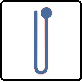
\includegraphics[angle=0,width=0.1\linewidth,keepaspectratio='true']{figures/du.png}}] DU, denoting a check mark: Show main menu 
\item[\raisebox{-1em}
{
\includegraphics[angle=0,width=0.1\linewidth,keepaspectratio='true']{figures/up.png}}] U: Zoom in 
\item[\raisebox{-1em}
{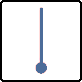
\includegraphics[angle=0,width=0.1\linewidth,keepaspectratio='true']{figures/down.png}}] D: Zoom out 
\item[\raisebox{-1em}
{
\includegraphics[angle=0,width=0.1\linewidth,keepaspectratio='true']{figures/left.png}}] L: Turn screen page pro-grade (Normal, Aux., Full-screen...) 
\item[\raisebox{-1em}
{
\includegraphics[angle=0,width=0.1\linewidth,keepaspectratio='true']{figures/right.png}}] R: Turn screen page retrograde (Normal, Full-screen...) 
\item[\raisebox{-1em}
{
\includegraphics[angle=0,width=0.1\linewidth,keepaspectratio='true']{figures/urdl.png}}] URDL, denoting a P: \textbf{P}an-mode. Might also be invoked by 
moving two fingers apart on the screen.
\end{itemize}
\vspace{2em}

\subsection*{More gestures available:}
\begin{itemize}
\item[\raisebox{-1em}
{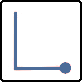
\includegraphics[angle=0,width=0.1\linewidth,keepaspectratio='true']{figures/dr.png}}] DR, denoting an L: Show the Select Waypoint dialogue similar to menu 
item Waypoint \textbf{L}ist
\item[\raisebox{-1em}
{
\includegraphics[angle=0,width=0.1\linewidth,keepaspectratio='true']{figures/rd.png}}] RD, denoting a T: opens the \textbf{T}ask Manager
\item[\raisebox{-1em}
{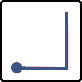
\includegraphics[angle=0,width=0.1\linewidth,keepaspectratio='true']{figures/dl.png}}] DL: show the Alternates List
\item[\raisebox{-1em}
{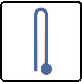
\includegraphics[angle=0,width=0.1\linewidth,keepaspectratio='true']{figures/ud.png}}] UD: enables Auto-Zoom
\end{itemize}
\vspace{2em}

\subsection*{Sophisticated dialogues:}
\begin{itemize}
\item[\raisebox{-1em}
{
\includegraphics[angle=0,width=0.1\linewidth,keepaspectratio='true']{figures/urd.png}}] URD, denoting an A: Show the \textbf{A}nalysis dialogue.
\item[\raisebox{-1em}
{
\includegraphics[angle=0,width=0.1\linewidth,keepaspectratio='true']{figures/ldrdl.png}}] LDRDL, denoting an S: Open the \textbf{S}tatus dialogue
\end{itemize}


%%%%%%%%%%%%%%%%%%%%%%
\chapter{Navegação}\label{cha:navigation}
Este capítulo descreve o mapa dinâmico e sua ajuda para a navegação, também descreve algumas informações de planeio e provas sobrepostas no mapa.

\section{Elementos mostrados no mapa}

\begin{maxipage}
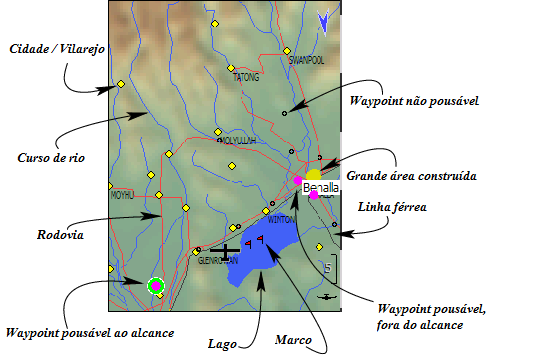
\includegraphics[angle=0,width=0.9\linewidth,keepaspectratio='true']{figures/fig-map.png}
\end{maxipage}

O mapa dinâmico mostra: 
\begin{enumerate} 
\item Aeronave, indicador de vento, perfil da termal, indicador de planeio final
\item Terreno, planícies e planaltos
\item Topografia, rios, rodovias e cidades
\item Waypoints, aeroportos e pousos
\item Prova ativa, zonas de observação e pilões
\item A direção (ou rota\footnote {A linha até o próximo waypoint pode ser uma {\em rota}, como descrição na seção~\ref{sec:route}.}) para a direção para o próximo waypoint.
\item Espaços aéreos
\item Marcadores, histórico de termais, trilha
\item Alcance do planeio\footnote{O alcance do planeio também é citado como
  {\em alcance}, assim como descrito na seção ~\ref{sec:reach}.}
\end{enumerate}
O mapa é desenhado em um sistema de coordenadas projetadas (sem latitude e longitude), e a escala pode ser alterada (zoom + e zoom -), bem como deslocado.  Todas as funções de navegação levam a curvatura da Terra em consideração.

\section{Símbolo do planador, orientação do mapa}
O símbolo do planador mostra a posição da aeronave no mapa.  A orientação da aeronave indica a direção estimada que a aeronave está apontando.

O mapa é orientado de três formas: norte acima, trilha acima e alvo acima.  O ajuste da configuração pode ser utilizado para especificar uma orientação diferente no mapa quando estiver em modo de círculos.  É bem útil para prevenir a desorientação quando olhar o mapa girando.  O modo alvo acima facilita determinar em qual direção se deve sair da termal.

Quando o modo trilha ou alvo acima é usado no modo de círculos, o símbolo da aeronave é centralizado na tela, mesmo que o símbolo seja configurado de outra forma.  No modo de cruzeiro, a orientação de trilha e alvo acima permite que o símbolo da aeronave seja posicionada (ex. 20\%) na parte inferior da tela, fornecendo uma boa visão do mapa à frente da aeronave.  Esta posição é definida nos ajustes da configuração.  

\section{Zoom e escala do mapa}\label{sec:zooming}

Para alterar a escala do mapa, dependendo do hardware, você usa:
\begin{enumerate}
\item Toque/clique em uma parte vazia do mapa para sublinhar o mapa se já não estiver selecionado.  Então utilize a roda do mouse ou as teclas acima/abaixo do Pocket PC para zoom + ou zoom -.
\item Um dispositivo PNA com um botão rotativo permite que se altere o zoom.
\item Dispositivos Android tem o +/- que permite que se altere o zoom.
\item Você pode também fazer o gesto para mudar o nível de zoom. Gesto acima (veja à esquerda) aumento o zoom.  Para baixo diminui o zoom.\gesturespec{up}
\item Ou selecione a função através do menu.
\begin{quote}
\bmenug{Mostrar 1}\blink\bmenug{Zoom In} e \bmenug{Zoom Out}
\end{quote}
\item No Altair, o botão rotativo pode ser usado para alterar o zoom.
\end{enumerate}

A escala do mapa é mostrada no canto inferior do mapa dinâmico.  A distância indicada é medida da borda esquerda para a direita do mapa dinâmico.
Usuários do Compaq Aero:  Se você ativar as teclas de jogo do Compaq Aero (no Menu-Q), os dois botões centrais serão as teclas acima/abaixo.
\marginpar{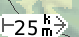
\includegraphics[angle=0,width=0.4\linewidth,keepaspectratio='true']{figures/zoom.png}}

Usuários do Compaq Aero:  Se você ativar as teclas de jogo do Compaq Aero (no Menu-Q), os dois botões centrais serão as teclas acima/abaixo.

\subsection*{Zoom Girando}
Há uma facilidade de ter dois tipos de zoom: um quando a aeronave está em modo girando e outro em modo de cruzeiro ou modo final.  Esta é a opção de Zoom girando, nos ajustes das configurações.  Por padrão, o zoom girando é ajustado em 2,5 – 5,0km dependendo do tamanho da tela.  Quando o usuário altera o zoom, afeta diretamente o zoom atual somente.  Quando se sai do modo atual de zoom, é usado o modo prévio de zoom. Se o modo de Zoom girando não está ativo, haverá somente um único nível de zoom.  Esta situação conduz a diferentes níveis de zoom sendo preservados para serem alterados manualmente, independentemente dos ajustes de Auto Zoom.
 
\subsection*{Auto Zoom}
Auto Zoom automaticamente aproxima a tela quando se está aproximando de um waypoint para manter a visualização em uma distância apropriada. 
\marginpar{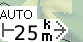
\includegraphics[angle=0,width=0.4\linewidth,keepaspectratio='true']{figures/zoomauto.png}} 
Quando o Auto Zoom está ativo, ‘AUTO’ aparece perto da escala do mapa.

Para ativar o Auto Zoom, use o gesto \gesturespec{ud} ou o menu descrito à esquerda. Para voltar ao zoom normal, faça o zoom manualmente, não importando o que já foi feito por menu ou gesto. 

\menulabel{\bmenug{Mostrar 1}\blink\bmenut{Zoom}{Auto}}
Quando um waypoint muda (automaticamente, através do seletor de prova ou manualmente selecionando waypoints), o Auto Zoom ajusta o nível de zoom automaticamente para que o próximo waypoint seja visível no mapa.

Durante o modo Girando se uma termal foi detectada, o mapa é centrado sobre a termal ou parte dela para que a aeronave continue sendo visível.
 
\section{Navegando no mapa (Panning)}\label{sec:panning}

O modo panorâmico permite ao usuário explorar áreas que estão além da aeronave.  É bem útil quando se está planejando a prova.
\begin{enumerate}
\menulabel{\bmenug{Mostrar 1}\blink\bmenug{Pan On}}
\item Ative o modo panorâmico por menu ou gesto.  O gesto para este modo é mover sua ponta do dedo acima, direita, abaixo e esquerda, formando um “P”. 
\gesturespec{urdl}
\item O mapa pode ser movido arrastando a tela ou usando as teclas.  Para Altair, modo panorâmico é feito com o botão rotativo interno/externo.  
\item Quando feito, o modo panorâmico pode ser desabilitado manualmente, pressionando PAN OFF no sub-menu.
\end{enumerate} 

\sketch{figures/pan.png}
Quando o modo panorâmico está ativo, as letras ‘PAN’ aparecem próximas à escala do mapa.  Enquanto estiver nesse modo, o foco estará na mira no meio do mapa.

Apesar de aparecer a mira (para usuários Altair), o mapa continuará oferecendo a opção “Oque Aqui?” tocando em qualquer posição no mapa (na tela de toque). 


\section{Waypoints} \label{sec:waypoint-schemes}
Os waypoints são mostrados com símbolos diferentes, dependendo do tipo do waypoint; a maior diferença são waypoints pousáveis e não pousáveis.

\subsection*{Pousáveis}
Os símbolos dos waypoints são desenhados conforme abaixo.  Há três conjuntos de ícones disponíveis para waypoints pousáveis. \config{waypointicons}

\begin{tabular}{c|ccc|ccc|}
Conj. Ícones 
&\begin{sideways}Pousável\end{sideways}
&\begin{sideways}Marginal\end{sideways}
&\begin{sideways}Alcançável\end{sideways}
&\begin{sideways}Aeródromo\end{sideways}
&\begin{sideways}Marginal\end{sideways}
&\begin{sideways}Alcançável\end{sideways}\\
\hline
Círculo Roxo &

\includegraphics[width=0.8cm]{icons/winpilot_landable.pdf} &

\includegraphics[width=0.8cm]{icons/winpilot_marginal.pdf} &

\includegraphics[width=0.8cm]{icons/winpilot_reachable.pdf} &
\colorbox{white}{
\includegraphics[width=0.8cm]{icons/winpilot_landable.pdf}} &

\includegraphics[width=0.8cm]{icons/winpilot_marginal.pdf} &

\includegraphics[width=0.8cm]{icons/winpilot_reachable.pdf} \\
\hline
Branco e Preto &

\includegraphics[width=0.9cm]{icons/alt_landable_field.pdf} &

\includegraphics[width=0.9cm]{icons/alt_marginal_field.pdf} &

\includegraphics[width=0.9cm]{icons/alt_reachable_field.pdf} &
\colorbox[rgb]{0.94,0.94,0.94}{
\includegraphics[width=0.9cm]{icons/alt_landable_airport.pdf}} &

\includegraphics[width=0.9cm]{icons/alt_marginal_airport.pdf} &

\includegraphics[width=0.9cm]{icons/alt_reachable_airport.pdf} \\
\hline
Luzes de tráfego &

\includegraphics[width=0.9cm]{icons/alt2_landable_field.pdf} &

\includegraphics[width=0.9cm]{icons/alt2_marginal_field.pdf} &

\includegraphics[width=0.9cm]{icons/alt_reachable_field.pdf} &
\colorbox{white}{
\includegraphics[width=0.9cm]{icons/alt2_landable_airport.pdf}} &

\includegraphics[width=0.9cm]{icons/alt2_marginal_airport.pdf} &

\includegraphics[width=0.9cm]{icons/alt_reachable_airport.pdf} \\
\hline
\end{tabular} \\

Os ícones marginais são desenhados para aqueles waypoints que estão principalmente no alcance, mas não é possível a aproximação direta (ex. uma montanha não permite a aproximação direta).
  
Os waypoints são rotulados opcionalmente de acordo com suas abreviações, esquemas e visibilidade.

No topo dos waypoints pousáveis, pode haver mais detalhamento.  Se houver a opção ativada 
`{\it Detalhar Pousáveis}' você terá informações adicionais quando houver a visualização deste waypoints.

\begin{enumerate}
\item  Campos pousáveis têm ícone quadrado apesar de serem mostrados em tabela.  O quadrado é desenhado como um diamante em pé.  Aeródromos permanecem com um círculo, facilitando sua visualização. 
\item  Todo o conjunto de ícones, incluindo o conjunto de “círculos roxos”, colocam a pista em suas atuais direções.  A direção da pista está disponível nos dados do waypoints.  Ex. os waypoints de formato (\verb|.cup|) não incluem esta informação.
\end{enumerate}

\subsection*{Pousáveis ao Alcance}
Próximo aos pousáveis, há uma estimativa da altitude acima da altura de segurança dos pontos pousáveis e é mostrada próxima ao waypoints.  Esta característica é uma das capacidades mais poderosas do XCSoar.  A altitude de chegada é calculada configurando-se o computador de planeio do XCSoar com parâmetros de polar, ajustes de MacCready, vento, abertura do terreno e altitudes de segurança.  Com tudo isso sendo configurável, há muito espaço para erros, portanto:

A menos que tenha entendido completamente os conceitos de cálculo de planeio, você deve \warning manter a pré-configuração do XCSoar (já julgado e fortemente aprovada).

É da responsabilidade do piloto sempre interpretar a leitura e observar os valores com o tempo.  Todavia, tendo ajustado o computador de planeio seguindo o Capítulo 
\ref{cha:glide} mostra a altitude estimada de alcance, desenhada ao lado de campos pousáveis ao alcance levam em consideração o relevo ou mostram ambos.
\config{arrivalheight}

Outra opção é mostrar o planeio médio necessário para um campo pousável ao alcance.  Este cálculo é derivado da distância atual ao campo pousável dividido pela diferença de altura entre a altura atual e a altura do campo pousável.  Novamente, a altura de segurança é adicionada à altura do campo pousável, mas nada mais é levado em consideração: sem vento, sem polar, sem ajuste MacCready, só geometria.  O conceito do planeio médio necessário é amplamente discutido, como um conceito bem robusto.

\tip Tenha em mente que necessita de um forte conhecimento dos dados de alcance e ajustes no computador de planeio.

\subsection*{Não Pousáveis}
Como o arquivo de waypoints contém informações da natureza do campo não-pousável, o mapa mostrará ícones específicos para estes pontos.  A tabela contém uma relação dos ícones de mapas apresentados (veja figura  \ref{fig:nonlandables}).

\begin{figure}[h]
\centering
\vspace{2.5cm}
\begin{tabular}{ccccccccc}
\begin{rotate}{60}Waypoint simples\end{rotate} &
\begin{rotate}{60}Topo da montanha\end{rotate} &
\begin{rotate}{60}Obstáculo\end{rotate} &
\begin{rotate}{60}Passagem\end{rotate} &
\begin{rotate}{60}Planta ou fábrica\end{rotate} &
\begin{rotate}{60}Torre ou prédio\end{rotate} &
\begin{rotate}{60}Túnel\end{rotate} &
\begin{rotate}{60}Estação metereológica\end{rotate} &
\begin{rotate}{60}Ponte\end{rotate}\\


\includegraphics[width=0.5cm]{icons/map_turnpoint.pdf} &
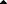
\includegraphics[width=0.8cm]{icons/map_mountain_top.pdf} &
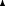
\includegraphics[width=0.7cm]{icons/map_obstacle.pdf} &
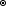
\includegraphics[width=0.7cm]{icons/map_pass.pdf} &
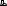
\includegraphics[width=0.8cm]{icons/map_power_plant.pdf} &
\includegraphics[width=0.7cm]{icons/map_tower.pdf} &
\includegraphics[width=0.6cm]{icons/map_tunnel.pdf} &
\includegraphics[width=0.6cm]{icons/map_weather_station.pdf} &
\includegraphics[width=0.8cm]{icons/map_bridge.pdf} \\

\end{tabular}
\caption{não pousáveis}\label{fig:nonlandables}
\end{figure}

\section{Prova ativa}

O curso da prova ativa é desenhado no mapa em linha azul (pontilhada).  As áreas atribuídas às provas mostram os setores dos pilões ou áreas sombreadas em amarelo.  Círculos são desenhados ao redor dos pontos de início e fim, as linhas são desenhadas nos pontos de início e fim se os pontos são deste tipo.  Os setores de observação da prova são desenhados em segmentos de círculos.

A todo tempo, uma linha fina é desenhada da aeronave até o próximo waypoint da prova.  Esta linha deve ser um caminho direto ao waypoint, ou ser uma rota livre de terrenos e espaços aéreos, descritos anteriormente em detalhes na seção
~\ref{sec:route}.

\begin{center}
\begin{tabular}{c c c}
{\it Início/Fim} & {\it Setor} & {\it Cilindro} \\
\includegraphics[angle=0,width=0.3\linewidth,keepaspectratio='true']{figures/cut-startfinish.png} &
\includegraphics[angle=0,width=0.3\linewidth,keepaspectratio='true']{figures/cut-sector.png} &
\includegraphics[angle=0,width=0.3\linewidth,keepaspectratio='true']{figures/cut-barrel.png} \\
\end{tabular}
\end{center}


\section{Terreno e Topografia}\label{sec:terrain_topo}

As seguintes características de topografia são desenhadas no mapa:
\begin{itemize}
\item Rodovias principais, mostradas em linhas vermelhas
\item Rios, mostrados em linhas azuis
\item Grandes corpos de água (lagos), mostrados em áreas azuis
\item Cidades grandes, mostradas em áreas amarelas
\item Áreas de pequena população, mostrada como diamantes amarelos 
\end{itemize}
Cidades e pequenas áreas com população são rotuladas em itálico.

O solo é colorido de acordo com a elevação e opcionalmente sombreado pelo sol ou pela direção do vento.  Solos inválidos ou abaixo do nível do mar são coloridos em azul.


\menulabel{\bmenug{Mostrar 2}\blink\bmenut{Terreno}{On/Off}}
\menulabel{\vspace{1cm}\bmenug{Mostrar 2}\blink\bmenut{Topo.}{On/Off}}

O solo é sombreado para melhorar a visibilidade.  O sombreamento padrão é ajustado coincidindo a iluminação virtual com a direção do vento, sendo as áreas mais brilhantes são barlavento e as áreas mais escuras são sotavento.   
A inclinação solar também foi implementada.  Se o sombreamento da encosta for ajustado para ‘Sol’, o brilho da encosta segue conforme o dia e hora.  A quantidade de sombra sobre o brilho do terreno é ajustável \config{shading}.

A visualização do solo e topografia podem ser acionados ou não através do menu.

\begin{tabular}{c c}
Topografia & Terreno \\
\includegraphics[angle=0,width=0.4\linewidth,keepaspectratio='true']{figures/cut-topo.png} &
\includegraphics[angle=0,width=0.4\linewidth,keepaspectratio='true']{figures/cut-terrain.png} \\
\end{tabular}

Se os dados do solo não estiverem disponíveis (ou a visualização estiver desligada), a cor de fundo do mapa será branca.  Todo o solo abaixo do nível médio do mar é mostrado em azul.  Se você estiver voando fora da terra, o fundo da tela será branco.  

\subsection*{Rótulos do mapa}\label{sec:maplabels}

A tela pode ser mais clara desligando a visualização dos rótulos de topografia e waypoints for a da prova escolhendo o menu ‘Rótulos’.
\menulabel{\bmenug{Mostrar 2}\blink\bmenut{Rótulos}{Nenhum}}

Outra opção para deixar mais clara incluem:

\jindent{\bmenuth{Rótulos}{Prova \&}{locais pouso}}{  Mostra rótulos para os waypoints na prova ativa e campos pousáveis (baseado nos atributos dos waypoints).  Os outros waypoints serão mostrados, mas sem rótulos. }

\jindent{\bmenut{Rótulos}{Prova}}{ Mostra somente os rótulos dos waypoints da prova ativa.}
\jindent{\bmenut{Rótulos}{Todos}}{ Mostra todos os rótulos para todos os waypoints.}

Note que em todos os casos, a formatação dos rótulos é configurável no menu
`{\it Waypoint Display}'.  \config{labels}


\section{Rastro}\label{sec:trail}


Um rastro opcional pode ser desenhado no mapa dinâmico para mostrar o caminho da aeronave.  A cor e a espessura do rastro dependem de altitude ou do valor do variômetro.


\begin{center}
\includegraphics[angle=0,width=0.5\linewidth,keepaspectratio='true']{figures/snail.pdf}
\end{center}

Se houver conexão do Vega ou outro variômetro inteligente com a saída Netto, o valor do vário Netto é usado; conseqüentemente as cores e a espessura do rastro indicarão o movimento vertical da massa de ar ao invés do movimento vertical da aeronave.

\config{snailtrail}
A visualização do rastro pode ser ajustada entre Desligado, Curto (+/- 10 minutos), Longo (+/- uma hora) ou Completo que mostrará todo o vôo.  Isto pode ser ajustado através dos ajustes de configuração ou temporariamente através do menu.
\menulabel{\bmenug{Mostrar 2}\blink\bmenut{Trilha}{Completo}}

Observe que para todos estes modos, o rastro é curto no modo Girando para facilitar a visualização.

De modo a auxiliar a centralização das térmicas na presença de vento, o rastro pode ser artificialmente derivado com o vento conforme vai sendo mostrado (é a compensação de deriva).  Deste modo, o rastro é referenciado pelo vento e não pelo solo.  Assim como as termais também são derivadas com o vento, o rastro pode dar uma indicação mais precisa onde esteve a aeronave com relação às termais.

O exemplo é ilustrado abaixo.  Observe que, quando a compensação da deriva do vento está ativa (figura à direita), a aeronave aparenta estar girando em uma coluna ao invés de estar em uma espiral alongada (figura à esquerda).

\begin{center}
\includegraphics[angle=0,width=0.6\linewidth,keepaspectratio='true']{figures/traildrift.png}
\end{center}

\config{traildrift}
Ativando a compensação da deriva do rastro é através dos ajustes de no menu de configuração. A compensação só é feita no modo Girando; a visualização do rastro no modo Cruzeiro não é afetada.  Também pode ser alterada pela janela de ajuste do vento.
\menulabel{\bmenug{Config 1}\blink\bmenus{Vento}}

A visualização do rastro é útil também para mostrar mais claramente quando as termais são cisalhadas pelo vento.
A largura da trilha pode ser opcionalmente alterada de acordo com a visualização do variômetro.  


\section{Marcadores}\label{sec:markers}

Os marcadores são mostrados como pequenas bandeiras no mapa.  Os marcadores podem ser adicionados manualmente ou automaticamente.  Um exemplo de como estes marcadores podem ser adicionados automaticamente é quando se entra em modo Girando, um modo simples de mostrar as termais encontradas.

\menulabel{\bmenug{Nav 2}\blink\bmenut{Marca}{Ponto}}
Os marcadores não são mantidos após o XCSoar ser fechado, porém a localização dos marcadores é anexada ao arquivo
 \verb|xcsoar-marks.txt|.

\section{Termais}

Enquanto estiver girando em termais, automaticamente será gerado um marcador e mantido até o \sketch{figures/thermalhistory.png} fim do vôo.  Este histórico termal é acessível através da função de elementos de mapa, da mesma forma que os marcadores ou waypoints.


\section{Linha de alcance de planeio}\label{sec:reach}

Uma linha de alcance de planeio é mostrada no mapa como uma linha pontilhada branca e preta, indicando onde a aeronave poderá pousar em terreno aberto.  O alcance é mostrado em todas as direções, incluindo caminhos obstruídos no terreno.  Esta opção é útil para conhecer o planeio relativo à topografia quando se está baixo e procura por termais, ou quando está voando em áreas montanhosas.

Os cálculos para o alcance podem ser configurados \config{turningreach} em dois níveis: 
\begin{description}
\item[Linha reta] se o alcance em curva está desabilitado, mostrará a maior distância que a aeronave pode voar no planeio final em todas as direções sem fazer curvas.  O alcance aparece como um anel fechado ao redor da aeronave.  

\begin{center}
\includegraphics[angle=0,width=0.8\linewidth,keepaspectratio='true']{figures/reach1.png}
% CUTOUT SHOWING GLIDE RANGE FOOTPRINT.  NO TOPOGRAPHY, FULLSCREEN, NO TASK. TURNING=FALSE
\end{center}

\item[Girando] se o modo Girando estiver ativo, o planeio será mostrado como a maior área que a aeronave pode alcançar em todas as direções, mesmo permitindo curvas ao redor de obstáculos.  A área de alcance aparece com um anel fechado ao redor da aeronave mas também pode incluir buracos indicando picos de montanhas que a aeronave não pode alcançar sem subir.

\begin{center}
\includegraphics[angle=0,width=0.8\linewidth,keepaspectratio='true']{figures/reach2.png}
% CUTOUT SHOWING GLIDE RANGE FOOTPRINT.  NO TOPOGRAPHY, FULLSCREEN, NO TASK. TURNING=TRUE
\end{center}

\end{description}

A tela pode ser configurada também para desfocar as áreas não alcançáveis fora do alcance do planeio da aeronave.  O caminho do planeio final é verificado levando-se em consideração também a abertura do terreno através do caminho e também a altura do terreno.
Se a abertura (clareza) do terreno não é atingida, aparecerá uma cruz vermelha no mapa onde a área é perigosa.  Se um alvo for definido, os cálculos são feitos através do caminho reto para o alvo.  Se não há alvo definido, o cálculo é feito através do caminho que está seguindo.
Se o alcance estiver ativo, o modo de aborto de prova usará os waypoints pousáveis e abrirá uma lista também com os waypoints alternativos do mapa.
Observe que os cálculos da prova não são afetados pelos cálculos de alcance – por exemplo, não são levados em conta os dados de altitude necessária para finalizar a prova e dados mostrados nas infoboxes.

Além do mais, os cálculos são usados para o anel de alcance, altura de chegada para waypoints pousáveis, modo de aborto e janelas de diálogo alternativas.  O desempenho da aeronave e os ajustes de MacCready usados nestes cálculos são configuráveis\config{reachpolar}:
\begin{description}
\item[Prova] O valor de MC é o usado na prova.
\item[Safety MC] Um valor de MC baixo pode ser configurado para ser usado como referencial ao melhor planeio da aeronave.  O grau de segurança alcançado nos cálculos é feito com a diferença entre o melhor desempenho de planeio e o planeio seguindo o MacCready de Segurança (speed to fly).  
\end{description}

\section{Abas de estado `{\it Voo}' e `{\it Tempo}'}\label{sec:flight-status}

A janela de diálogo Estado é multi-tabular, fornecendo uma visão geral da informação do vôo, sistema, prova, regras e tempos.  Pode ser acessada com o gesto “S” ou com o botão do Menu. 
\gesture{Esquerda - Baixo - Direita - Baixo - Esquerda}
\begin{quote}
\bmenug{Info 2}\blink\bmenug{Estado}
\end{quote}

\subsection*{Vôo}
Selecione a página `{\it Flight}'. 
A janela mostra a localização da aeronave e pode ser útil quando se reporta a posição.  Mostra a posição da aeronave, o máximo ganho de altura, waypoints mais próximo, ângulo de direção e distância.
\sketch{figures/status-flight.png}

Você pode achar esta função útil quando for reportar sua localização para outros pilotos ou resgate.

\subsection*{Tempo}\label{sec:time-status}
Seleciona a aba  `{\it Times}'. 
Mostrará a hora local, tempo de vôo, hora da decolagem e pouso e hora do nascer e pôr do sol.

Observe que estes valores nesta aba são estáticos e só serão atualizados a cada abertura de aba. 
\sketch{figures/status-times.png}
Para ver os dados atualizados, é necessário fechar a aba e abrí-la novamente.  Os valores serão atualizados automaticamente a cada abertura desta janela.  Familiarize com este procedimento antes de realizá-lo em vôo.


\section{Rota}\label{sec:route}

O XCSoar pode planejar caminhos pelo terreno e obstáculos no espaço aéreo em três dimensões da aeronave até o destino.  Este caminho é conhecido como rota.  A altura do destino é a altura de chegada para waypoints finais ou pode ser mais alto para waypoints intermediários, se forem regras da prova ou requisitos para completar a prova.  

As funções de planejamento de rota são ordenadas por modo de prova, modo de aborto e modo ‘ir para’.

\begin{center}
\includegraphics[angle=0,width=0.8\linewidth,keepaspectratio='true']{figures/route3.png}
\end{center}

As rotas levam em consideração o desempenho da polar e são calculadas para levarem o mínimo tempo.  Por padrão, os cálculos de rota são desativados e podem ser ativados somente por solo ou quando na prevenção de espaço aéreo. \config{routemode}

O solo é evitado verticalmente pela altura de segurança do terreno \config{safetyterrain}, sem nenhuma abertura de terreno lateral.  As rotas válidas podem  resultar na chegada da aeronave ao destino mais alta que a altura mínima – como pode ocorrer quando o destino está além de uma montanha mais alta.

O espaço aéreo é evitado horizontalmente por uma margem de aproximadamente 250m sem nenhuma abertura imposta verticalmente.  As rotas válidas podem voar acima ou abaixo do espaço aéreo.

Se o MacCready é positivo, a subida é opcionalmente permitida nos cálculos de rota.  O topo da subida deve ser limitado a 500m acima do teto de início e final, ou incluso no teto, definido pelo teto da termal \config{routeceiling}.  As subidas acima da altitude de início e final são penalizadas por uma taxa de subida mais lenta que o valor de MacCready atual.

Algumas aproximações e limitações do sistema de planejamento de rotas são:
\begin{itemize}
\item Quando subidas são necessárias (e permitidas) para alcançar o destino, as subidas podem ocorrer no início da rota. 
\item Segmentos de subidas em cruzeiro podem ocorrer em altitude constante, equivalente a muitas pequenas subidas distribuídas ao longo do caminho. 
\item Falhas sobre o resultado dos cálculos podem se reverter em vôo direto da aeronave, de sua localização atual para o destino.
\end{itemize}



%%%%%%%%%%%%%%%%%%%%%%
\chapter{Cross Country Tasks}\label{cha:tasks}

XCSoar provides a full task management system, in which tasks can be
edited prior to flight and, when undertaking casual cross-country
flying, modified during flight.  Waypoints are advanced automatically
or may be cycled through manually. Many of XCSoar's computations relate to
either turnpoints or the finish waypoint.
Unless a "true" task is defined, XCSoar will provide a "go home" function, with 
many of the task related functions referring to the location of takeoff.
This chapter also describes the use of IGC loggers with XCSoar.

There are three task modes available:
\begin{description}
\item[Ordered task] This is the natural cross-country task type,
in which the task consists of a start point, zero or more waypoints,
and a finish point.  The task points are to be flown in order.
\item[Goto task] Flight to a single destination.
\item[Abort task] Provides options to fly to the nearest landing points.
\end{description}

Note that in goto and abort modes, the ordered task is retained and may be resumed
later, preserving any statistics about achievement in the task.

\subsection*{Automatic goto}

If no ordered task is defined, then on takeoff, a goto task is automatically
established with the takeoff point as the destination, or the nearest airfield
if it was close to the takeoff point.

Whether or not a task is defined, the takeoff point is always
generated and appears in the waypoint list for later reference or use.

After having defined an ordered task for the very first time, the automatic "goto takeoff" function is skipped. To resume a simple task, use goto.

\section{Goto tasks}

Goto tasks may be established by selecting a waypoint from the map,
the waypoint list, or any other mechanism e.g. the alternates dialogue, 
and select \bmenuw{Goto}. In goto task mode, selecting
\bmenug{Nav 2}\blink\bmenug{Task Resume} resumes the ordered task (if
any).

\section{Editing tasks}

You can edit tasks in several ways.  Some methods are more useful for
editing prior to flight, and others allow tasks to be modified whilst
in flight for casual cross-country touring.  Tasks can be saved to
files and reloaded later, and can be transferred between any XCSoar
platform (Pocket PC, Altair, PC).

\tip It is also possible to save a `default' task and have this task loaded
automatically upon start-up of XCSoar.  One application of this is to
set up a default task with one waypoint being the home --- this means
that XCSoar is then programmed for final glide back to home, which is
useful for casual cross-country touring.

The main ways of setting tasks are the following:
\begin{itemize}
\item Using the task editor dialogue
\item Selecting waypoints from the map and adding them to the task from the
 waypoint details dialogue
\item Loading the task from a file
\end{itemize}

%Selecting the Task menu item will produce the Task dialogue box.  The
%list box on the left displays all of the turn points loaded into the
%system. Highlight the desired entries and using the "-$>$" and "$<$-"
%buttons assemble the desired task in the Task list box. As each turn
%point is added to the task a continuous display of the calculated task
%length is shown.  Tasks can be saved for recalling later using the
%"Save" button and recalled using the "Load" button.  Once the desired
%task is complete select "OK".
%
%{\it DIAGRAM SHOWING TASK DIALOG EDITING, WITH LABELED ARROWS POINTING
%TO THE USER INTERFACE ELEMENTS?}

Loading a task from file may be useful in competition or casual
cross-country flying in groups, as one person can distribute the task
file to others, thereby saving effort on editing the task severalfold.
\tip
If no task is present at startup, a task is created automatically,
containing one waypoint takeoff as ``goto home''.

XCSoar saves the current task when shutting down and loads it at
startup, thereby allowing the task to be entered early in the day,
then the device running XC Soar can be turned off until flight time.

Task waypoints are preserved even if the waypoint
file is changed.  This means, if you save a task, then change the
waypoint file, then load the task again, new waypoints are generated
for any waypoints that are missing in the new waypoint file.

\section{Waypoint Information}
%Several ways of selecting a waypoint are available:
%\begin{itemize}
%\item Touch its name or the waypoint symbol on the map screen if it is visible.
%\item If the waypoint is in the active task, highlight the waypoint {\InfoBox}, 
%  then use the up/down arrow keys to select the desired waypoint, and press the
%enter key.
%\item From the Task dialogue, find and highlight the waypoint in
% the waypoint list, then press the 'Details' button.
%\end{itemize}
%The display will now show the waypoint details dialogue.

The waypoint info dialogue describes a waypoint in detail and has
navigation functions such as GoTo, insert, append to the task, or set the 
waypoint as the new home.
This may be accessed in several ways:

\gesturespec{rd}or menu \bmenug{Nav 1/2}\blink\bmenug{Task},
\todonum{descr. tabular "Turn Points"}
highlight a waypoint, then tap the highlighted waypoint again to display the 
task point dialogue, then push \bmenuw{Details}.

\gesturespec{dl}or menu \bmenug{Nav 1/2}\blink\bmenug{Alternates}
to show the
details of the landables nearest to the aircraft.

\gesturespec{dr}or menu \bmenug{Nav 1/2}\blink\bmenug{Waypoint List}
, highlight and \bmenuw{select} a waypoint to show its details.

\gesturespec{urdl}or menu \bmenug{Display 1/2}\blink\bmenug{Pan On} to put the 
map into pan mode, pan to the desired waypoint, touch its name or the waypoint 
symbol.

\bmenug{Info 1/3}\blink\bmenug{What's here?}
to show the
item list under the cross-hair, or your index finger on the map.

The waypoint details dialogue contains two major pages (accessed via the
\bmenuw{$>$} and \bmenuw{$<$} buttons). Depending on the availability of further
details of the waypoint they will by shown on extra pages.

\subsection*{Waypoint details}\label{sec:waypointdetails}
This page contains text describing the waypoint's location, radio frequency and 
runway information (if this information is in the waypoint file) elevation, 
local daylight time, bearing and distance to the waypoint, and the altitude required 
to reach the waypoint as described below. In addition, there is a button 
\bmenuw{GoTo} to directly initiate
navigating to this waypoint. The button cancels the current task. 
\begin{center}
\includegraphics[angle=0,width=0.8\linewidth,keepaspectratio='true']{figures/dialog-waypointdetails0.png}
\end{center}

As mentioned above, the Waypoint info dialogue also shows three forms of altitude 
difference (additional
altitude required to reach the waypoint at the safety height) for
the corresponding waypoint:
\begin{description}
\item[Alt diff MC 0] Altitude difference at MC setting of 0
\item[Alt diff MC safety] Altitude difference at the abort/safety MacCready 
  setting (see \ref{sec:safety-factor})
\item[Alt diff MC current] Altitude difference at the current MacCready setting
\end{description}

From the main Waypoint Info screen, you can access the second page by using the 
\bmenuw{$>$} and \bmenuw{$<$} buttons in the bottom left corner of the page.
\subsection*{Task actions menu}  
This page contains a column of buttons allowing various actions to be performed:
\begin{description}
\item[\bmenuw{Replace in task}] replaces the active waypoint in the task with 
  the selected waypoint.
\item[\bmenuw{Insert in task}] inserts the selected waypoint before the active 
  waypoint in
  the task.
\item[\bmenuw{Append to task}] adds the selected waypoint to the end of the task.
\item[\bmenuw{Remove from task}] removes the selected waypoint from the task.  
  Note that this option is only visible if the selected waypoint is included in 
  the active task.
\item[\bmenuw{Set as new home}] sets the waypoint as the home airfield.
\item[\bmenuw{Pan to waypoint}] switches to pan mode and pans to that waypoint.
\end{description}

It is a good idea to set your home waypoint from the waypoint details
dialogue. This causes XCSoar to start up at the home location regardless
of whether a GPS fix is received.  If no home is set, then XCSoar
starts in the centre of the terrain map.

\subsection*{Airfield information}
This page may contain relevant text from the enroute supplement about
the airfield, including runways, radio frequencies, traffic patterns,
contacts.
\begin{center}
\includegraphics[angle=0,width=0.8\linewidth,keepaspectratio='true']{figures/dialog-waypointdetails1.png}
\end{center}

\subsection*{Waypoint details image}
This page shows a satellite image of the waypoint.

\begin{center}
\includegraphics[angle=0,width=0.8\linewidth,keepaspectratio='true']{figures/dialog-waypointdetails2.pdf}
\end{center}
How to set up the detailed waypoint information read section \ref{sec:airfield-details}

\section{Waypoint selector dialogue}\label{sec:waypoint-selector-dialog}

The waypoint selector is a dialogue that allows waypoints to be easily selected
from a potentially large database. \gesturespec{dr}

Invoking the selector brings up a filtering dialogue screen with a set of 
\menulabelr{\bmenug{Nav 1/2}\blink\bmenug{Waypoint List}}
optional filters on the left side of the page, and a list of waypoints on the
right, matching all of the filtering conditions set.
There are several filters available, which may be used together,
individually or not at all.
\begin{description}
\item[Name] Selects waypoints, starting with the string typed.
\item[Distance] Filters out waypoints farther than a specified distance from the 
  aircraft.
\item[Direction] Filters out waypoints that are not in a specified direction 
  from the aircraft. 
  An additional special direction ``HDG(0°)'' filters waypoints within 30
  degrees to either side of the heading of the glider.  This allows the pilot 
  to point the glider at a group of waypoints and quickly find them.
\item[Type] Filters out waypoints that are not of the specified type
(Landable point, Airport or Turnpoint) or that appear in the specified File~1 or
File~2 (primary or secondary waypoint file respectively).
\end{description}
When filtering by name and type, the list of matching waypoints is
sorted by name. When (in addition) filtering by distance or direction,
 the list of matching waypoints is sorted by distance.

\begin{center}
\includegraphics[angle=0,width=0.8\linewidth,keepaspectratio='true']{figures/dialog-waypointselect.png}
\end{center}

The list can be scrolled if there is more than one screen full of
matching waypoints.  To scroll through the list, simply drag with the finger, or
move to the bottom (or top) of the list with the cursor.   

Selecting an item will result in different behaviour
depending on what function opened the waypoint selector.  In typical
use it brings up the waypoint details dialogue for the selected
waypoint.

\section{Task manager}\label{sec:task-manager-dialog}
\begin{it}  The task manager has undergone significant redesign compared with 
earlier versions of XC Soar.\end{it}
\gesturespec{rd}

The task manager is used to edit, view, load, save to file, and declare cross
country tasks.
\menulabelr{\bmenug{Nav 1/2}\blink\bmenug{Task}}

The primary page is a calculator. It shows various calculations 
related to the active task, as described in detail below.  In addition, there 
are buttons for invoking dialogues \bmenuw{Turn Points}, \bmenuw{Manage}, 
and \bmenuw{Rules}, as well as a button to \bmenuw{Close} the task manager.

\subsection*{Task calculator dialog}\label{sec:task-calc-dial}
The task calculator dialogue allows the pilot to see the effect of
various changes to the task on final performance.
\menulabelr{\bmenuw{Calculator}}

In flight the Task Calculator might also be accessed from the Analysis pages. 
With pages Task, Climb, and TaskSpeed a button \bmenuw{Task Calc} comes up, 
that directly changes to the Task Calculator screen.


\begin{center}
\includegraphics[angle=0,width=0.8\linewidth,keepaspectratio='true']{figures/dialog-taskcalculator.png}
\end{center}

\begin{description}
%\item[Assigned task time]  This field displays the assigned task time.
\item[Estimated task time]  This field displays the estimated total time 
  on task to complete the task at the provided MacCready setting.
\item[Task distance]  This field displays the task distance remaining.
\item[Set MacCready]  Allows the user to adjust the MacCready value and 
  see the effect it has on the estimated task time.
\item[AAT range]  Allows the user to adjust the targets within the remaining 
  AAT areas, to see the effect it has on estimated task time and task distance.
\item[Speed remaining]  This field displays the estimated speed for the
  remainder of the task at the provided MacCready setting.
\item[Achieved MacCready]  This field displays the achieved MacCready value.
\item[Achieved speed]  This field displays the achieved speed % at the achieved MacCready setting???
\item[Cruise efficiency]  100 indicates perfect MacCready performance, greater 
than 100 indicates better than MacCready performance is achieved through flying
in streets. Less than 100 is appropriate if you fly considerably off-track. This 
value estimates your cruise efficiency according to the current flight history 
with the set MC value. Calculation begins after task is started.
\end{description}
See Section~\ref{sec:task-speed-estim} for more details on task speed
and achieved MacCready calculations.

On closing the dialogue the entered MacCready value is used as the MacCready 
setting. If the \bmenuw{Cancel} button is pushed, the MacCready setting is 
unaffected.

The \bmenuw{Target} button, for AAT tasks, adjusts the range
(increases or decreases) so that the estimated task time exceeds the
assigned task time by less than five minutes.  The range is adjusted
target-wise. In typical use, all targets are set to ``auto" that means the pilot 
does not have to manually adjust the range to find the course for arrival at 
the assigned task time, thereby reducing pilot workload.

\subsection*{Turn Points}
This page displays an ordered list of the points in the current active task.
\menulabelr{\bmenuw{Turn Points}} 
If there are no waypoints in the active task, there 
will be only an option to "Add Turnpoint."  By highlighting (tapping) the 
"Add Turnpoint" function, then tapping in the highlighted region, the waypoint 
selector is displayed, as described above.  Highlighting a waypoint from the 
list and then tapping on the highlighted region adds the waypoint to the task.

\subsection*{Manage}
This page allows for invoking all operations needed to create new or manage 
\menulabelr{\bmenuw{Manage}}already defined tasks.


\begin{itemize}
\item [\bmenuw{New Task}] Clears the current task and resets the task rules to 
  the default values.
\item [\bmenuw{Declare}] If an external logger is connected, this will allow 
  uploading the  active task to the logger and declaring it.
\item [\bmenuw{Browse}] Displays a list of all the saved tasks, allowing the 
  pilot to load a previously saved task.  Note that this option will overwrite 
  the current active task.
\item [\bmenuw{Save}] Saves the current active task.  Upon tapping the 
  \bmenuw{Save} button the pilot will be prompted to enter a file name for the 
  task to be saved.
\end{itemize}

\subsection*{Rules}
The values in the menu depend on the task type selected. Clicking any existing 
\menulabelr{\bmenuw{Rules}} value will bring up another menu allowing the pilot to select a 
different value for this rule.  Task types are discussed in more detail below.

Also, tapping on the \bmenuw{Rules} button again after it is highlighted allows 
toggling between a "thumbnail" view of the task map and a larger view of the task.

\section{Task types}
XC Soar currently defines three different task types: Racing, AAT, and FAI badges/records.

A brief description of the task types is included below, but this manual does 
not intend to rephrase FAI rules or contest task types. The reader is encouraged 
to become thoroughly familiar with each task type by referring to contest rules 
or FAI rules, which are available at \url{http://www.fai.org}. 


\subsection*{Racing}
(also known as an "assigned task").  The racing task involves flight 
around each specified turnpoint in the specified order.  Selecting the racing task 
type allows the pilot to enter the following parameters.
  \begin{description}
  \item [Arm start manually] If set to ``On'', some extra buttons are presented 
  in order to let you \bmenug{Arm start} as well as \bmenug{Disarm start} in 
  menu \bmenug{Nav 1/2}, controlling  the detection of the start condition.
  \item [Start open time] This is the time when the start zone opens.
  \item [Start close time] This is the time when the start zone closes.
  \item [Start max. speed] This is the maximum speed allowed in the start observation 
    zone.  This should be set to 0 if there is no limit.
  \item [Start max. height] This is the maximum height above the start height 
    reference (AGL or MSL) at which a task can be started.  This  should be set to 
    0 for no limit.
  \item [Start height ref.] This specifies whether the maximum start height is 
    referenced to ground level of the start point ("AGL") or Mean Sea Level ("MSL").
  \item [Finish min. height] This is the minimum height based on the finish 
    reference (AGL or MSL) at which a task can be finished.  This should be set to 
    0 for no limit.
  \item [Finish height ref.] This specifies whether the minimum finish height 
    is referenced to ground level of the finish point ("AGL") or Mean Sea Level ("MSL")
% \item [FAI start/finish rules] If enabled, this task type has no max. start height 
%   or max. start speed.  Finish height reference is set to AGL and finish height 
%   is 1000m below the start height \todonum[inline]{Is this description correct?}
  \end{description}
  
\subsection*{Assigned area task (AAT) and Modified area task (MAT)}
(also known as "Turn Area Task,"or TAT).  This is a task through assigned 
areas (restricted to cylinder or sector observation zones).  A minimum task time 
applies.  Rules options for this task type include:
  \begin{description}
  \item [AAT min. time]  This is the required minimum time for the task.  Refer 
    to contest rules or consult an expert for penalties associated with finishing 
    prior to the minimum time.  The time in this option is given in minutes.
  \item [other rules] All other rules stay the same as in case of task type 
    ``racing''.
  \end{description}


\subsection*{FAI badges/records}
  \begin{description}
  \item [FAI start/finish rules] If set to ``On'', only start times might be set. 
  If set to ``Off'', all other racing task rules might be altered from the FAI standard.
  \end{description}

Once the appropriate task type has been selected and start and finish rules 
have been defined as described above, it is necessary to define the properties 
of each waypoint in the task.  

\section{Turn Points' task rules}\label{sec:task-rules}

The \bmenuw{Turn Points} dialogue brings up the list of waypoints in the task. 
\menulabelr{\bmenuw{Turn Points}} If no waypoint is already defined, this screen 
will show an empty list. With \bmenuw{(add Turnpoint)}, up and down arrows, and 
\bmenuw{Make Finish} an ordered list of waypoints is created. 
Waypoints can be start point, turnpoint, or finish point.
Highlighting any waypoint on the list and either tapping it again or 
touching the \bmenuw{Edit Point} button brings up the waypoint definition. 
Touching \bmenuw{Change type} will bring up a menu of the various task point 
types available.  Definitions of each point type are given below.

A variety of task rules may be used when specifying tasks, including
the common FAI triangles and Assigned Area Tasks (AAT).  Many aspects
of the rules can also be customised.

Starting and finishing lines are centred on their associated waypoint
and aligned perpendicular to the next and previous waypoints
respectively.

Sector turn-points are 90 degree segments aligned to the bisection of
the previous and next waypoints, as commonly used in FAI tasks.
There is also support for British BGA, and German DAeC sectors.

\subsection*{Start point types}
The conditions to be met for a valid start depend on the type of start:
\begin{description}
\item[Start Cylinder] When the glider leaves the cylinder area.
\item[Start Line] When the glider crosses the start line.
\end{description}

\subsection*{Turnpoint types}
The conditions to be met for a valid turnpoint pass depend on its
 type:
\begin{description}
\item[FAI Sector] When the glider has entered the observation zone (OZ), defined 
by a segment and radial distance from the waypoint.  The segment is
defined by a 90 degree arc centred about the bisector of inbound and
outbound legs, with a distance of 20 km.
\item[Keyhole Sector (DAeC 0.5/10 sector)] When the glider has entered the
observation zone, defined by a segment and radial distance from the waypoint.  The segment is
defined by a 90 degree arc centred about the bisector of inbound and
outbound legs, with a distance of 10 km.  The observation zone also includes
a cylinder of 500 m.
\item[Turnpoint Cylinder]  When the glider has entered the observation zone
defined by a radial distance from the waypoint.
\item[BGA Fixed Course Sector]  When the glider has entered the
observation zone defined by a segment and radial distance from the
waypoint. The segment is defined by a 90 degree arc centred about the
bisector of inbound and outbound legs, with a distance of 20 km.
The observation zone also includes a cylinder of 500 m (British rules).
\item[BGA Enhanced Option Fixed Course Sector]  When the glider has entered the
observation zone defined by a segment and radial distance from the
waypoint. The segment is defined by a 180 degree arc centred about the
bisector of inbound and outbound legs, with a distance of 10 km.
The observation zone also includes a cylinder of 500 m (British rules).
\item[Area Zylinder (AAT)]  and
\item[Area Sector (AAT)]  When the glider has entered the observation zone
defined by the radial distance from the waypoint, and segment for sector areas.
\end{description}

\subsection*{Finish point types}
Task completion depends on the finish type:
\begin{description}
\item[Finish Cylinder] When the glider enters the cylinder area.
\item[Finish Line] When the glider crosses the finish line.
\end{description}

Automatic advancement is triggered whenever a condition is met. To start an AAT,
mixed task, or Racing task the start has to be armed before. 

\tip Competition rules may be defined in a profile file for
distribution to a group of pilots or task-setters, so all competitors
are playing by the same rules!

Additional task rules for valid starts and finishes may also be
specified.  Starts may have a defined maximum altitude above ground,
and a maximum speed.  Finishes may have a minimum altitude above
ground.  These parameters are defined in the page ``Default Task Rules'' in
the configuration \config{taskrules} settings.

For non-AAT tasks, an option is available to set the minimum finish
altitude according to the FAI rule, whereby the minimum finish
altitude is above 1000 meters below the start altitude.


%Need to add a section describing how to start the task%


\section{Advancing and restarting tasks}\label{sec:advanc-rest-tasks}
At all times one waypoint in the task is designated as the active
waypoint.  The active waypoint is used for calculation and display of
navigation information, that is, the pilot is directed to fly towards
the active waypoint (also referred to as the ``next waypoint'' in the
description of InfoBoxes as in Chapter~\ref{cha:infobox}).

During flight a continuous display of the bearing to the next waypoint is shown.

The altitude required to complete the task is calculated for the route starting
from the glider's actual position going through the task's turnpoints to the 
final waypoint.

Changing the active waypoint is performed automatically, or may be performed manually.
The start point of racing tasks, and AAT task points, are special cases that require
the task point to be ``armed'' before the system will automatically advance to the next
task point once that point is reached.  All other task points will automatically
advance to the next point as soon as the last point was reached.

For non-racing tasks, no user interaction is required to
advance through the task --- the system will automatically advance as
each task point is achieved.  The user may still manually advance or retreat the active
task point by selecting the menu items \bmenug{Nav}\blink\bmenug{Previous turnpoint} and
\bmenug{Nav}\blink\bmenug{Next turnpoint} respectively.

The menu items \bmenug{Previous turnpoint} and
\bmenug{Next turnpoint} show dynamic labels that
indicate the action that will be performed upon selecting the item.

For task points requiring arming, \bmenug{Next Turnpoint} becomes 
\bmenug{Arm turn} if the turn is not armed; if it is armed, then it becomes 
\bmenug{Next Turnpoint} allowing for manual advance. 
\bmenug{Previous Turnpoint} changes to \bmenug{Disarm turn} if the turn is armed 
and vice versa. Similarly, for racing tasks these menu items update for arming 
start points. If the Next Turnpoint is the \bmenug{Finish Turnpoint}, the menu 
label changes accordingly.

Status messages are given for task points requiring arming, when
inside the observation sector, as reminders to arm the turn when the
pilot is ready to advance to the next waypoint. For starting, a
warning is given that the glider is in the start cylinder or behind
the start line, as a reminder to ``arm'' if necessary.

For PC and Pocket PC with touchscreen versions only, the user may
manually cycle through the waypoints by highlighting the waypoint
{\InfoBox} and by pushing the up or down cursor key.

See Section~\ref{sec:task-rules} for details on observation rules.

If a user has cycled through the waypoint manually, this does not mean
that the glider has successfully passed the waypoint!  However, this
facility is useful to force a task restart or to skip a waypoint when
flying a casual cross-country task.

\tip Tasks can be restarted simply by manually cycling back through the
waypoints to the start.

In all modes, if the glider re-enters the start zone or crosses the
start of the previous start, the task will be automatically restarted. 

When selecting \bmenug{Previous turnpoint}, the trigger that detects
auto-advance for that waypoint is cleared; meaning that the task
manager expects the aircraft to fly to that observation zone (OZ)
again before continuing the task. The pilot may still select \bmenug{Next
turnpoint} to advance to the next task waypoint.

A system beep and message is given on task/waypoint advance.  The
messages are given when the system advances the task waypoint
automatically or, in manually arm mode, when the system is armed and the
aircraft is in sector:
\begin{description}
\item[Task start]  appears when the aircraft has crossed the start line or
 exited the start sector. This can be repeated any time.
\item[Next turnpoint]  appears when the aircraft has entered the observation
 sector for turnpoints. Turns with variable target advance as soon as
 \button{Arm Turn} is pushed.  For the manual arm mode, if the
 aircraft has already entered the observation sector and left, pushing arm will
 cause the task manager to expect, that the turn is intended to approach
 another time.
\item[Task finish]  appears when the aircraft has crossed the finish line
 or entered the finish cylinder.  This occurs in both advance modes. 
\end{description}


\section{Alternate starts}\label{sec:alternate-starts}

%Alternate start points are skipped for XCsoar 6.0, but
%will potentially brought back in a next release. 

%\todonum[inline]{Alternate start points are skipped for XCsoar 6.0, but
%will potentially brought back in a next release. This section can thus be
%treated as obsolete. }

The task system allows alternate start sectors to be defined:

\blink\bmenuw{Turn Points} select start point, \menulabelr{\bmenug{Nav 1/2}\blink
\bmenug{Task}}\bmenuw{Edit Point}\blink\bmenuw{Enable Alternate Starts}

On the start point edit page of the Task Manager turn on the \bmenuw{Enable 
Alternate Starts} property. Another screen is brought up for defining an 
alternate start point. In case, alternate start points have been defined before, label \bmenuw{Enable Alternate Starts} changes to \bmenuw{Edit Alternates}. After selecting ``Add Alternate Start'' and touching 
\bmenuw{Relocate} the ``Select Waypoint'' filtering dialogue is invoked.

Having set up several alternate start points, the ``next waypoint'' scheme again will be extended. Before detection of a valid start and having armed start manually, the menu buttons stepping through all the waypoints will show label \bmenug{Next Start}.

Summarizing, all dynamic menu labels in menu \bmenug{Nav 1/2} show commands to be 
executed for selecting waypoints and conditions either consecutively or in reverse 
order. 

%\begin{center}
%\includegraphics[angle=0,width=0.8\linewidth,keepaspectratio='true']{figures/%dialog-startpoint2.png}
%\end{center}
  
%  To edit the start points, move the cursor to an item in the list on
%  the right side of the dialogue, and press enter.  This opens the
%  waypoint selector dialogue, to allow selection of the waypoint.  This
%  process can be repeated several times for several alternate start
%  waypoints.  Press the `clear' button to clear all alternate start
%  points.

%  Each start sector is fixed to the same type (line/cylinder) and size
%  (start radius) defined in the task waypoint page.

%  Note that the task start point should be included in the alternate
%  start location list. 

%\begin{center}
%\includegraphics[angle=0,width=0.8\linewidth,keepaspectratio='true']{figures/%dialog-startpoint3.png}
%\end{center}

%\begin{center}
%\includegraphics[angle=0,width=0.8\linewidth,keepaspectratio='true']{figures/%dialog-startpoint4.png}
%\end{center}

%  In flight, any time you cross a start line (or exit a start
%  cylinder), this will start the task at that particular alternate
%  start.  Task statistics are recalculated for the start sector you
%  last flew through.  All alternate start sectors are shown on the
%  map.  You can re-start simply by flying through the start sector
%  again or another start sector.  This automatic re-start will only
%  happen if the active waypoint is the first turnpoint after the
%  start, or the start itself.

%  When the waypoint advance mode is `Arm' or `Arm Start', then a start
%  is only recognised by XCSoar if the advance trigger is armed.

%  If desired, alternate start points may be selected as the active
%  waypoint by selecting the previous waypoint.  Continuing to select
%  the previous waypoint will cycle through all alternate start points.

\section{Abort/resume the task and Alternates}

If atmospheric conditions change for the worse, you may make the
judgement that it will be impossible to complete the task.  In this
situation, XCSoar can be instructed to ``abort'' the task, and it will
then help you reach a safe landing site. An ordered task can be aborted in 
different ways. Either it is done by selecting a waypoint and execute the goto 
command or by invoking the abort mode. In either case, the ordered task might be resumed.

\subsection*{Task Abort}\label{sec:taskabort}
Invoking the abort mode forces XCSoar to enter a special case of the final glide mode. \menulabelr{\bmenug{Nav 2/2}\blink\bmenug{Task Abort}} For a discussion on 
flight modes refer to section \ref{sec:flightmodes}. In this flight mode
the configuration option `reach polar' determines whether
waypoint arrival heights in abort mode uses the MacCready value prior
to aborting the task, or if the safety MacCready value is used. \config{reachpolar}
Default is to use the safety MacCready value.  When switching to
abort mode, the MacCready setting is set to the safety value 
if it is lower than the current setting.

With invoking abort mode the cross-country task is disabled. On the map radials 
are drawn pointing to the nearest landables to instantly 
support the pilot's decision. As is during the whole flight, the group of nearby 
landables is maintained permanently. Radials and nearest landables may change 
dynamically when in abort mode, so that at any time several landing options are 
presented and any of these may be selected as the active waypoint. Even if no 
landable is in reach, the radials are drawn.
\sketch{figures/abort-low.png} 
If conditions improve, the task can be resumed by selecting the same
menu button that aborted the task, now denoting \bmenug{Resume Task}. The active 
waypoint, prior to aborting the task, is then restored along with all the other 
task details.

\subsection*{Alternates} \label{sec:alternates}
Alternates are maintained throughout the flight, reflecting good airmenship by 
always keeping an eye on possible alternates.\menulabelr{\bmenug{Nav 1/2}\blink
\bmenug{Alternates}} Six landing 
options are maintained. They are filtered by the configured ``alternates mode'' 
criteria (Simple, Task, or Home). \config{alternatesmode} 
Choosing Task or Home puts some bias on the presentation of alternates to the 
heading, you were taking whilst still task oriented.

As is with every waypoint list, additional information might be called by tapping \bmenuw{Details} before deciding which final to go. Select a waypoint from the list and push \bmenuw{Goto}.
\sketch{figures/alternates_list.png}

Although the items on the alternate list obey different rules they interact 
in the same way 
with the current task. Choosing a target from the alternates list aborts the task; 
once the conditions get better the resuming of the task is doable by the already 
mentioned button.


\section{Task status}\label{sec:task-status}

The status dialogue gives a summary of important task information. 
\gesturespec{ldrdl} It can be useful to give a
good overview of the task status while freeing up InfoBoxes for other
purposes.  The status dialogue can be referred to in order to confirm
that a valid start was detected, as well as the progress against the
task.
\menulabelr{\bmenug{Info 2}\blink\bmenug{Status}}
The status dialogue can be invoked by menu or gesture left down right down left, denoting an S. The status tabs `Task' and `Rules' are of interest.

The task tab shows the AAT times, distances achieved and remaining and the 
task speeds. The rules tab shows the validity of start/finish according 
to the task rules.
\begin{center}
\begin{tabular}{c c}
Task & Rules \\
\includegraphics[angle=0,width=0.4\linewidth,keepaspectratio='true']{figures/status-task.png} &
\includegraphics[angle=0,width=0.4\linewidth,keepaspectratio='true']{figures/status-rules.png} \\
\end{tabular}
\end{center}

\section{Assigned Area Tasks}\label{sec:aat-tasks}

\subsection*{AAT targets}

A {\em target} is a point within an AAT area that the pilot intends to
fly to.  These targets can be moved within the AAT areas so the pilot
can adjust the effective distance of the task.  Targets may be set on
the ground, during task planning, and modified during flight.

When flying an AAT task, the navigation system directs the glider to
the target, and statistics like distance to waypoint are also relative
to the target rather than the waypoint of the AAT area itself.

Automatic task waypoint advancement does not trigger when entering an
AAT area solely. The pilot has to arm the turn manually to advance to the next
turn. When arming the AAT turn while flying through the OZ also the task
optimiser is triggered to capture the realized AAT target and bring the target
optimisation for the rest of the task up to date. See Section~\ref{sec:advanc-rest-tasks} 
for details.

\subsection*{Manually moving targets}

In order to make the specification of targets more straightforward,
their location is defined by a range parameter that determines how
far from the minimum to maximum possible distance the target is.  This
is expressed as a percentage.  For example, with range set to 100\%,
the target is located to give the maximum overall task distance.  With
range set to~$-100$\%, the target is located to give the minimum overall
task distance.  

Zero range yields a nominal task distance: for sectors the target is
half way along the bisector radial; for cylinders the target is in the
center of the cylinder.

The task calculator dialogue (see Section~\ref{sec:task-calc-dial}), shows the
average percentage over all turns in the AAT Range field.
The targets can be individually modified from the target dialogue of the task
calculator.


\subsection*{AAT targets and the Task Calculator}

The typical use of targets in flying AAT is as follows:
\begin{itemize}
\item Set the expected MacCready, bugs/ballast and wind settings
  for the flight using the flight settings and wind settings dialogues.
\item Define the task as normal from the task editor.
\item Based on the pilot's judgement of how good the weather is,
  and whether some areas are likely to be more or less difficult than
  others, targets may be set individually for each turn-point in the
  target view.  The ETE field in the target view compared to
  the assigned minimum time is shown as Delta T to check if the planned 
  task is efficient and long enough.
\item During flight, if situations change, such as changed MacCready setting
  or wind, the task calculator can be brought up to show the estimated
  task time, again allowing comparison to the assigned minimum time.
\item If the pilot decides to extend or shorten the flight, all the remaining
  targets can be modified from the task calculator. 
\end{itemize}

The task calculator therefore allows the pilot to make (and help to
answer) `what if?' questions, for example:
\begin{itemize}
\item What will happen if the conditions improve?  The MacCready setting can be 
increased and the pilot can see if there is sufficient adjustment to targets in 
order to be able to extend the planned task.
\item What will happen if the conditions deteriorate?  The MacCready setting can 
be decreased and the pilot can see how much the task can be shortened and still 
finish the task later than the assigned minimum time.
\item What will happen if I leave the AAT area now?  By pressing \button{Arm
turn} the take over of the current position into the optimization can
be forced. The repositioning of subsequent turns can be reviewed in the task calculation
dialogue.
\end{itemize}

\subsection*{Target projection}

XCSoar continually analyses the path of the glider through AAT sectors
to find the points in previous AAT sectors through which the achieved
scoreable distance will be greatest.  Internally, the program moves
the targets for previous AAT sectors, which are then the optimal
targets.

In certain conditions, targets for the current AAT sector may be moved
automatically:
\begin{itemize}
\item When inside an AAT sector, the target in that sector is moved to
to a line projecting from the previous sector's target through the
aircraft, at the same distance from the previous sector's target to
the target prior to entering the sector.  The effect of this is to
allow pilots to choose to enter an AAT sector in a different direction
or offset from the direct line from the previous target to the current
target.

\item While the aircraft is in the AAT sector and the distance from the
previous target to the aircraft is greater than the distance from the
previous target to the current target, the target is moved further
along the projected line from the previous target to the aircraft,
just beyond the aircraft.  Hence, the black track line will not be
visible but the blue optimal track arrow will point along this
projected direction.
\end{itemize}

A worked example is provided in the following figures to illustrate
how targets move during a flight and to show how XCSoar determines the
maximum scored path.

\begin{maxipage}
\begin{center}
\begin{longtable}{|c|c|}
\toprule
\includegraphics[angle=0,width=0.45\linewidth,keepaspectratio='true']{figures/faat01.png} & 
\includegraphics[angle=0,width=0.45\linewidth,keepaspectratio='true']{figures/faat02.png} \\
{\em Outside sector} & {\em Inside sector} \\
Target (-20\%) is on bisector & Target moved along track line \\

\midrule
\includegraphics[angle=0,width=0.45\linewidth,keepaspectratio='true']{figures/faat03.png} & 
\includegraphics[angle=0,width=0.45\linewidth,keepaspectratio='true']{figures/faat04.png} \\
{\em User decreased range} & {\em User increased range} \\
Target (-80\%) moved along track line & Target (80\%) moved along track \\

\midrule
\includegraphics[angle=0,width=0.45\linewidth,keepaspectratio='true']{figures/faat05.png} & 
\includegraphics[angle=0,width=0.45\linewidth,keepaspectratio='true']{figures/faat06.png} \\
{\em Analysis (task page)} & {\em Next waypoint} \\
Path around active target  & ``Arm Turn'' pressed \\
\bottomrule
\end{longtable}
\end{center}
\end{maxipage}

\begin{maxipage}
\begin{center}
\begin{longtable}{|c|c|}
\toprule
\includegraphics[angle=0,width=0.45\linewidth,keepaspectratio='true']{figures/faat07.png} & 
\includegraphics[angle=0,width=0.45\linewidth,keepaspectratio='true']{figures/faat08.png} \\
{\em Analysis (task page)} & {\em Approaching next area} \\
Best scored target found & Target (60\%) is on bisector \\

\midrule
\includegraphics[angle=0,width=0.45\linewidth,keepaspectratio='true']{figures/faat09.png} & 
\includegraphics[angle=0,width=0.45\linewidth,keepaspectratio='true']{figures/faat11.png} \\
{\em Inside sector} & {\em Next waypoint} \\
Target (60\%) moved along track line & ``Arm Turn" pressed \\

\midrule
\includegraphics[angle=0,width=0.45\linewidth,keepaspectratio='true']{figures/faat12.png} &  \\
{\em Analysis (task page)} &  \\
Best scored targets found &  \\

\bottomrule
\end{longtable}
\end{center}
\end{maxipage}

\section{OnLine Contest}

The analysis dialogue contains a page `OnLine Contest' which can be
used to show the optimal path and estimated score.  The configuration settings \config{taskrules} 
(task rules page) allows the selection of which set of rules to be used for the
OLC optimisation.

The optimization is done continuously in the background and can be retrieved at
any time. The analysis page shows a graphical overview of the optimisation
result besides distance and score. A InfoBox is available which gives the
instant OLC distance and score as well.

\begin{center}
\includegraphics[angle=0,width=0.8\linewidth,keepaspectratio='true']{figures/shot-olc.png}
\end{center}

When flying OLC, either AAT or non-AAT tasks may still be used to
manage the flight navigation.  During flight, the computer will optimise the
current flight with respect to the selected OLC rules.  

In the OLC analysis page, the aircraft track is shown as a thin green line, the optimal 
path is shown as a thick red line.

The score and computed optimal distance is approximate.

When the aircraft has landed, the displayed result gets not updated anymore.


\section{Logger}\label{sec:logger}

A flight logger conforming to the IGC file specification can be used
to record flights.  

Several flight loggers are accessible via XCSoar:
\begin{itemize}
\item A software-based logger.  All versions of XCSoar have this
  functionality.  The logger conforms to the IGC standard but is not
  certified.
\item For example the PRO version of Altair has an internal IGC certified logger 
  device.  XCSoar communicates with the logger as to any other external device.
\item XCSoar can also send declarations to some external logger devices. 
  For this to work, the device must be specified in the `Devices' 
  section of the configuration \config{comdevices} settings.
\item  For some of the numerous logger devices XCSoar can download IGC files. 
  This is convenient especially for logger devices, which are not that easy 
  removable from the glider.
\end{itemize}

\subsection*{Setup}
For a complete matrix of the supported logger features see section~\ref{sec:supported-varios}.  
The configuration is described in detail in section~\ref{conf:logger}.  Details 
to the log files can be found in section~\ref{sec:logfiles}.

\subsection*{Logger activation}
The logger can be turned on and off automatically or manually.  For para-glider 
XCSoar provides the option to only start the logger automatically. Thus a very 
slow and close to the terrain flight won't automatically stop logging the flight. 
If you choose the auto start only logger you have to stop the logger manually.
To turn the logger on (or off) manually, select from the menu:
\sketch{figures/logger-startdeclare.png}
\begin{quote}
\bmenug{Config 3}\blink\bmenut{Logger}{Start}
\end{quote}

When the internal software logger is active, a small `green status led' in the
lower right corner of the map area flashes once per second.

By default, XCSoar is set up to automatically start and stop the
internal software flight logger when it detects the aircraft is flying
and when it has landed, respectively.  Only when the logger is
manually started does it ask if the flight is to be declared; when
automatically starting it automatically declares the current task.
In simulation mode the logger does not get activated automatically.

If a task has been declared, then subsequent attempts at modifying the
task result in a warning message asking to confirm whether the action
is to be taken and invalidate the declaration.  This is intended to
make it harder to accidentally modify the task resulting in a failed
declared task.

The XCSoar software logger, when started, checks for 500kB of free
space on the file storage.  If there is insufficient space, it will
automatically delete IGC files, oldest first, in order to free up
500kB.  It does not ask the user for confirmation before performing
this operation. \warning

The internal software logger buffers data so that when it starts
(automatically or manually) up to 60 seconds of data prior to starting
is recorded.  This means that the software logger now adequately
captures the full take-off.

\subsection*{Logger replay}\label{sec:logger-replay}
Flight logs in the IGC format generated by XCSoar or other loggers can
be replayed.  The logger replay dialogue can be accessed via the
menu:
\begin{quote}
\bmenug{Config 2}\blink\bmenug{Replay}
\end{quote}
\sketch{figures/loggerreplay.png}

During replay, the word `REPLAY' appears at the lower left corner of
the screen.  During replay, the program behaves as if real GPS updates
are being received by a GPS.  The logger replay dialogue does not need
to be open during replay.

To start a log replay, first select the file to load, and then select the
\button{Start} button.  The replay can be performed in accelerated time
by changing the time scale from 1x to a higher number, and paused by
setting the time scale to zero.  High time scales can result in degraded
performance of the wind estimation and other statistics/analysis routines.

Stop the log using the \button{Stop}.
Once a log is started, further presses of the \button{Start} has the
effect of restarting the replay.

\tip It is recommended to reset the device before flight, after a log
file has been replayed, in order to ensure that XCSoar's internal
statistics are properly reset.

When operating XCSoar in FLY mode, the replay is disabled (stopped) if
the real GPS receiver detects that the aircraft is moving.

The logger replay works best with high sampling rate log files;
a 6 second interval or less works fine.

\subsection*{Error analysis logger}\label{sec:raw-logger}
For the pure reason of tracking down error prone behaviour of XCSoar 
there is a `Raw Logger'. In case you are able to reproduce an error you can 
activate the raw log file creation by:
\begin{quote}
\bmenug{Config 3}\blink\bmenug{Raw Logger}
\end{quote}
Developers will appreciate very much any detailed error description including a log file like this. It really facilitates the root cause analysis and saves time to fix an error.

\section{Flight analysis} \label{sec:analysis-climb}

The analysis dialogue is very useful in planning and conducting
cross-country flights.  It is accessed via the menu:  \gesture{Up - Right - Down}
\begin{quote}
\bmenug{Info 1}\blink\bmenug{Analysis}
\end{quote}

Several pages are of interest:
\begin{description}
\item[Barograph]  Shows a graph of the history of the altitude of the glider.
  Statistics are used to estimate the thermal working band (average
  base and ceiling of climbs) and to estimate how the ceiling is
  changing over time.  The base and ceiling lines are drawn on the
  barograph.

  The `Settings' button opens the flight settings dialogue
  (e.g.\ to adjust the QNH)

\begin{center}
\includegraphics[angle=0,width=0.8\linewidth,keepaspectratio='true']{figures/analysis-barograph.png}
\end{center}

\item[Climb history]
  Shows a bar chart of the average climb rate achieved during each
  climb.  Statistics are used to estimate the overall average climb
  rate, and to estimate how this average is changing over time.  The
  current MacCready setting is drawn on the bar chart as a thick red
  dashed line, and the climb rate trend is drawn on the chart as a
  blue line.

  The ``Task Calc'' button opens the task calculator,
  (e.g.\ to adjust the MC value)

\begin{center}
\includegraphics[angle=0,width=0.8\linewidth,keepaspectratio='true']{figures/analysis-climb.png}
\end{center}

\item[Task]
  This page shows an overview of the entire task.  The main task line
  is drawn in thick dashed green, AAT areas are shaded.  For AAT
  tasks, the path from the aircraft around the remaining targets within AAT
  areas is shown in red.  The aircraft track is shown as a thin green line.

  The `Task Calc' button opens the task calculator,
  (e.g.\ to adjust the AAT task range or MC value)

\begin{center}
\includegraphics[angle=0,width=0.8\linewidth,keepaspectratio='true']{figures/analysis-task.png}
\end{center}

\end{description}

\section{Sunlight and time}

A sun ephemeris computes the time of sunrise and sunset, which is displayed in the
Aircraft Status dialogue (see Section~\ref{sec:time-status}).  Note that
local terrain and atmospheric conditions may result in poor visibility
before the displayed sunset time.

For PDA systems, the clock is adjusted for daylight saving time according
to the settings in the operating system.  For Altair, the clock UTC offset
must be adjusted manually for daylight saving time in the configuration
settings dialogue.

If the expected arrival time at the final waypoint in the task is past
sunset, a status message warning is issued.


%%%%%%%%%%%%%%%%%%%%%%
\chapter{Glide Computer}\label{cha:glide}
This chapter focuses on how XCSoar's glide computer works and is
recommended reading so you understand the specific details of
calculations being performed and how to use the software properly.  It
assumes a basic knowledge of cross-country soaring, but is suitable
reading for competition pilots as well as pilots engaging in casual
cross-country touring.


\section{Flight modes} \label{sec:flightmodes}

In order to reduce the pilot's workload, XCSoar is enabled to do 
different things depending on the actual flight's state. XCSoar can 
do this without in-flight interaction of the pilot. The differences are 
reflected by different displays, calculations, and flight information 
amongst others. The four states used by XCSoar are called 
\emph{flight modes}, which are
\begin{itemize}
\item Cruise mode
\item Circling mode
\item Final glide mode
\item Abort mode
\end{itemize}
XCSoar automatically detects the difference between circling flight and 
cruising flight. Circling is enabled when the glider turns (typically 
three quarters of a turn). After about 30 seconds of straight line flight 
the software will switch from circling to cruise mode. Hence, the switch 
is based on a simple condition.

It is also possible to have circling mode switched based on an external 
input (e.g.\ from a pilot-operated switch).

Final glide becomes active when the glider is above final glide 
path with respect to the given navigational task and safety margins. 
The required altitude depends most 
importantly on the adjusted MC value, but also the ground clearance 
is considered. On entering a thermal while in final glide mode for 
gaining some extra safety margin XCSoar will switch to the circling 
mode and back to the final glide mode, once the thermal is left again 
and the final glide condition is still met (i.e. the glider is still 
above the final glide path, considering MC setting and terrain).

As an example, a powerful feature to be driven by flight modes is the 
switch between different MacReady setting's strategies. If you decided 
to let XCSoar manage the setting automatically it will maintain a value 
based on past thermals worked out successfully until final glide. 
Instantly MacReady is set to achive minimal arrival time or what you 
set up for final glide (see section \ref{sec:auto-maccready}).
\config{final-glide} Hence the switch to final glide mode is based on 
a set of sophisticatedly computed tactical conditions.

You might force XCSoar to enter final glide mode by skipping all 
remaining turnpoints, if for example conditions get worse and you 
decided to just go home.

Abort mode is invoked manually to give you full control in case of 
emergency via menu.  No automatics - you decide.  The abort mode 
might be understood technically as a special final glide mode with 
concurrent support for multiple optional targets. However, in 
perception the abort mode simply supports your urgent decision where 
and how to go finally (see section \ref{sec:taskabort}).  In this case, 
a safety MacReady value is set. \config{safetyMC} Hence the switch to 
abort mode is based on the pilot's cognition.

Due to the fact, the different flight modes typically are reflected in 
differring things being displayed, the frequent XCSoar user might get 
used to some kind of watching a `display mode'. This is just the 
default \emph{perceived} after having installed XCSoar without having 
done some advanced configuration. As holds true for almost everything 
within XCSoar, the display's behavior might be changed adding value 
for the advanced user. But altering things in XCSoar does not influence 
the conditions for entering a flight mode, they do not change.

In order to take full advantage of the flight modes concept, XCSoar 
will \emph{always} show you, which mode is active. A small symbol is 
drawn on the lower right corner of the map area to indicate which flight 
mode the computer is in.

\begin{tabular}{c c c c}%{c c c c}
\includegraphics[angle=0,width=0.75cm,keepaspectratio='true']{icons/mode_cruise.pdf} &
\includegraphics[angle=0,width=0.75cm,keepaspectratio='true']{icons/mode_climb.pdf} &
\includegraphics[angle=0,width=0.75cm,keepaspectratio='true']{icons/mode_finalglide.pdf} &
\includegraphics[angle=0,width=0.75cm,keepaspectratio='true']{icons/mode_abort.pdf}\\
(a) & (b) & (c) & (d)
\end{tabular}

\begin{description}
\item[Cruise (a)]   The glider is not circling and there is either no 
task active, or the task waypoint is not the finish point.
\item[Circling (b)]  The glider is circling (though it may not be climbing).
\item[Final glide (c)]  The glider is not circling and the active waypoint 
is the final one in the task.
\item[Abort (d)]  This manually-triggered mode indicates the immediate 
landing options to the user.(see section~\ref{sec:taskabort})
\end{description}

The concept of different flight modes enables much more to be automated:
\begin{itemize}
\item \config{screenpages} The InfoBoxes may be set up differently for 
each flight mode. (see section \ref{sec:infoboxandpages})
\item \config{circlingzoom} Change zoom level between circling and other 
flight modes (this is called `circling zoom', see section\ref{sec:zooming}).
\item \config{variogauge} Switch the vario gauge's reading between Vario 
(gross climb rate) and airmass lift around you (net) whilst cruising 
(see section \ref{sec:variometer}).
\item \config{thermalassistant} When in circling mode, invoke the 
`thermal assistant', a small polar diagram depicting the updraft over 
circular course (see section \ref{sec:thermal-assistant}).
\item \config{traildrift} Switch to a so-called drift compensation, 
drawing a wind-compensated trail of the circles you fly to better depict 
wind shear (see section \ref{sec:trail}). 
\end{itemize}

Take notice, that this list is just an excerpt from an entirety of 
switchable items. You will find numerous dependencies conducted by the 
actual flight mode, whilst further reading this manual. Please pay 
attention to, because the flight mode concept is one of XCSoars 
fundamental basics. Another very basic scheme deals with how to structure 
informations to be displayed at once. These informations are grouped in 
\emph{screen pages} Further details are given in section 
\ref{sec:infoboxandpages} "Infoboxes and screen pages".\config{screenpages}


\section{MacCready setting}

The MacCready setting may be adjusted several ways:
\begin{itemize}
\item With \bmenug{Config 1}\blink\bmenug{MC $+$/$-$}
\item For touchscreen/mouse devices, select the MacCready InfoBox field, then
  use the up and down arrow keys.
\item When connected to a supported intelligent variometer, adjusting
  the MacCready setting on the variometer will change the setting
  in XCSoar according to the devices synchronisation configuration (see 
  section \ref{conf:comdevices})
\end{itemize}
In addition, an automatic MacCready mode is available as described in
section~\ref{sec:auto-maccready}.


\section{Glide polar}\label{sec:glidepolar}

The glide polar specifications of a wide selection of glider types,
representing major classes of gliders, are built into XCSoar.
\menulabelr{\bmenug{Config 2/3}\blink\bmenug{Plane}}
If your glider type is not listed, these may be used as an approximation for  
if no better glide polar can be found.  \config{polar} However, for most 
accurate results, it is advisable to use the correct glide polar for your particular
aircraft type. 
Besides the aircraft type the correct over all mass of the glider is important for 
accurate results. 
The preflight check of your tactical glide computer certainly 
includes a check of the correct settings for water ballast, with regard to the 
configured dry mass. Because XCSoar does not offer a setting for the pilots 
weight you are free to include the latter to the dry mass setting, or the 
water ballast setting.

On top of the polar and mass configuration the glide polar is adjustable 
in flight to take into account performance degradation due to bugs or 
rain droplets.

The build-up of bugs on the wing's leading edge, as well as rain
droplets on the wing, affect the aerodynamic performance.  It is the
pilot's responsibility to judge and update the bugs value during
flight.  The bugs value is expressed as a percentage of degradation 
compared to the clean glider's performance.  
For example, at 0\% bugs value, the glider
performs as a clean glider, and at 50\% bugs value, the glider's
sink rate is doubled when compared to a clean glider. The calculation 
scales linearly in-between. 

\menulabel{\bmenug{Info 1}\blink\bmenug{Analysis}}
\begin{center}
\includegraphics[angle=0,width=\linewidth,keepaspectratio='true']{figures/cut-clean-dirty-polar.png}
\end{center}
Knowing all this, a meaningful setting for a worst-case bug polluted wing could
scale down the polar by 30\%. Some experimentation may be required to determine 
appropriate settings for bugs, because the performance degradation experienced 
by different glider types may be different.

Alternatively, you can enable the "Auto bugs" feature which adds 1\% to the
bugs setting after each full hour of flying.   This feature is set via

\button{Config 2}\blink\button{System}\blink\button{Glide Computer}
\\*
\blink\button{Safety Factors}\blink\button{Auto bugs}\\

The ballast is set in litres of water. 
Depending on the specifically set dry mass of the glider, this may optionally 
include a weight margin to provide for different pilot weights.
  When flying with no ballast, a heavy pilot
may set a ballast value of perhaps 15 l so that the polar is
appropriately adjusted for the increased cockpit weight.

\begin{center}
\menulabel{\bmenug{Info 1}\blink\bmenug{Analysis}}
\includegraphics[angle=0,width=\linewidth,keepaspectratio='true']{figures/overlay-non-balasted-polar.png}
\end{center}


\section{Flight setup dialogue}\label{sec:flight-setup}
Use the flight settings dialogue to modify the all up weight of the glider both
before and during flight, as well as to set the QNH pressure.  

\menulabel{\bmenug{Config 1}\blink\bmenug{Flight}}
\begin{center}
\includegraphics[angle=0,width=0.45\linewidth,keepaspectratio='true']{figures/dialog-basicsettings.png}
\end{center}

The 'bugs' setting determines the amount the polar is degraded
due to contamination during a long flight.  A 'bugs' setting of 0\%
will cause the software to use the clean polar. A 'bugs' setting of
50\% will degrade the polar and effectively doubling the sink
rate for a given airspeed.

The ballast setting is used to modify the polar to account for any
water ballast carried during the flight. Ballast is shown in litres,
and should be set to correspond to the correct water ballast added
before flight.  The ballast setting modifies the polar to account for
the indicated load of water ballast.

Use this dialogue both before and during the flight to record the mean
sea level atmospheric pressure, also known as QNH pressure.  The
software uses the values entered to convert airspace flight levels
into altitudes.  If connected to a supported intelligent variometer
with an altimeter, the altitude is updated on this dialogue as the QNH
pressure is adjusted.  This makes it easy to set the QNH pressure if
the airfield elevation is known.

The maximum forecast ground temperature is used by the convection
forecast algorithm (see Section~\ref{sec:convection-forecast}) in its
determination of estimated convection height and cloud base.

\tip It is possible to configure XCSoar to display the basic
settings dialogue when it starts up.

On system startup, after the GPS has acquired lock, and if a
barometric altitude source is connected (e.g.\ Vega, AltairPro,
FLARM), the QNH is automatically adjusted.  This adjustment sets the
QNH such that the barometric altitude equals the terrain altitude.

The QNH is only updated if the aircraft is on the ground for more than
10 seconds, so that if XCSoar is restarted during flight, QNH will not
be adjusted.  The update only occurs also if the terrain database is
valid at the current aircraft location.

\section{Speed command display}

When used in conjunction with an intelligent variometer that produces
indicated airspeed measurements, a speed command chevron is drawn
on the right side of the map display.  If the glider is flying slower
than the optimal speed, the chevrons are red and point downwards.  If
the glider is flying faster than the optimal speed, the chevrons are
green and point upwards.  If the speed is approximately optimal, no
chevrons are drawn.

%{\it DIAGRAM SHOWING SPEED COMMAND CHEVRONS}

Depending on the configuration, speed command chevrons can be
displayed on the right side of the map area, or on the variometer
gauge.


\section{Speed to fly}\label{sec:stf}

XCSoar continuously calculates two types of speed to fly:
\begin{description}
\item[MacCready speed]  This is the best speed to fly during cruise
  in still air, adjusted for wind if in final glide mode.
\item[Dolphin speed]  This is the instantaneous, best speed to fly
  in rising or descending air, adjusted for wind if in final glide
  mode.
\end{description}  

The user can specify a maximum manoeuvring speed in the configuration
settings, which limits the speed-to-fly in MacCready calculations to
realistic values.

Different pilots have personal preferences as to whether they prefer
to fly in so-called `block MacCready' style, in which they fly
constant speed between thermals according to the MacCready speed; or
to fly in `dolphin' style, in which they fly at varying speeds
according to the continuously changing Dolphin speed value.

\begin{maxipage}
\begin{center}
\includegraphics[angle=0,width=0.8\linewidth,keepaspectratio='true']{figures/figure_speed_to_fly.pdf}
\end{center}
\end{maxipage}

A configuration option `Block speed to fly' (see
Section~\ref{sec:final-glide}) can be used to specify whether dolphin
or block speed to fly is used.  The infobox `V Opt' shows the optimum
speed according to whichever mode is selected.  When connected to the
Vega intelligent variometer, the speed command sounds are based on
this optimum speed value.


\section{Speed to fly with risk}\label{sec:safety-factor}

  The speed to fly system can be compensated for risk, in which the
  MacCready setting used for calculating the speed to fly (in both
  Block or Dolphin modes) is reduced as the glider gets low.

  Many pilots typically wind down the MC as they get low --- this
  feature performs this automatically.  The theory governing how this
  is implemented in XCSoar is based loosely on the paper by John
  Cochrane, ``MacCready Theory with Uncertain Lift and Limited
  Altitude'' {\em Technical Soaring} 23 (3) (July 1999) 88-96.

\url{http://download.xcsoar.org/papers/john.cochrane/safety_glides.pdf}

  A configuration parameter $\gamma$ (`STF risk factor', in the
  configuration settings under page `Glide Computer') controls how the
  risk MC value is calculated.  The $\gamma$ factor determines the
  fraction of the current MacCready setting as a function of the
  height fraction.  The height fraction used in this calculation is
  the ratio of the height above terrain ($h$) to the height of the
  maximum climb (this will usually be close to cloudbase) above the
  terrain ($h_{top}$).  The $\gamma$ setting thus represents the
  fraction of the total available climb (cloudbase minus terrain) at
  which you would wish to abandon the task and begin to prepare for a
  landout.  Thus, low $\gamma$ values indicate a higher tolerance for
  landout risk than higher values of $\gamma$.

  For the default value, $\gamma=0.0$, there is no compensation ---
  the risk MC is the same as the MC setting.  For $\gamma=1.0$, the
  risk MC is scaled linearly with the height fraction $h/h_{top}$.
  For intermediate values of $\gamma$, the risk MC varies smoothly
  with the height fraction, such that the risk MC is small only when
  low.

  Low values of $\gamma$ are best when pilots do not want to slow down
  as they get low (but risk out-landing); high values of $\gamma$ can
  be used for very cautious pilots but will result in lower average
  speeds.

  A value of $\gamma=0.3$ is recommended.

\begin{center}
\includegraphics[angle=0,width=\linewidth,keepaspectratio='true']{figures/riskmc.png}
\end{center}


\section{Safety heights}\label{sec:safety-heights}

Three safety heights are defined to provide a degree of safety margin
in glide computer calculations.  

The safety heights are:
\begin{description}
\item[Arrival height]  This is the elevation above ground at which
 the glider is required to arrive at least.
 Typically you want include height for a safe landing circuit, plus
 some safety margin for hazardous vertical/horizontal air movements and
 resulting errors of computed route and speed.
 This value is used in final glide calculations as
 well as the determination and display of reachable landable fields.
\item[Terrain clearance]
 This is the elevation above ground, below which any computed glide
 path is considered to provide inadequate clearance to the terrain.
 The terrain clearance value affects the glide range display, and if
 the final glide at any point dips below the terrain clearance
 elevation above ground, a warning marker (large red cross) is drawn
 on the screen.  If the terrain elevation model is invalid or out of
 range, then the glide range display and the terrain warning marker is
 disabled.
\item[Break-off height]  This is the elevation above ground, below which 
 it is recommended for pilots to consider the cross-country task
 failed and to concentrate on finding a suitable field to land in.
 Currently this break-off height does not affect XCSoar in any way but
 it is referenced in the manual.
\end{description}

\begin{maxipage}
\begin{center}
\includegraphics[angle=0,width=\linewidth,keepaspectratio='true']{figures/figure_terrain.pdf}
\end{center}
\end{maxipage}

\warning
These may be set to zero but this is highly discouraged since all
glide computers, instruments and data sources (such as terrain
elevation models) are subject to some degree of error and the
atmosphere through which the glider flies is also unpredictable.

XCSoar determines the elevation above sea level of any turn point or
landing point either from the waypoint file, or if no height is
specified in the waypoint file, from the terrain file.

\textbf{The estimated arrival altitude displayed next to landable
  waypoints is by default calculated for best glide angle at zero
  MacCready ring setting (MC$=0$), adjusted for wind.  However, a
  safety MacCready setting may be configured to modify the MacCready
  setting used in this calculation, as described below.}

Landable fields are only marked as reachable if the estimated arrival
elevation above ground is above the arrival altitude safety height,
and the glide path does not intersect the terrain clearance safety
elevation.

At all times, if the final glide through terrain marker (a red
cross) is displayed on the screen, then the glider must climb in order
to safely reach the destination.

When calculating the arrival heights of landable fields (for map
display purposes and in abort mode), a safety MacCready value can be
specified in the configuration settings.  This safety value is set to
zero by default.  Larger values make the arrival height calculation
more conservative.


\section{Final glide calculator}

The final glide calculator uses many sources of information when
determining the altitude required to reach your goal or the next
waypoint. These are:

\begin{itemize}
\item The glider's polar data;
\item The wind speed and direction;
\item The distance and bearing of the goal or waypoint;
\item The MacCready setting;
\item The altitude of the waypoint or goal;
\item A user specified safety margin (arrival height and terrain clearance).
\item The glider's total energy if XCSoar is connected to
  an instrument with an air speed indicator.
\end{itemize}

From the parameters shown above, two altitudes are derived.
\begin{description}
\item[Altitude required]
This calculation is the total altitude required for the glider to
reach the goal plus any user safety margin. 
\item[Altitude difference]
This calculation is the altitude required to glide to the goal plus
any safety arrival altitude plus the altitude of the goal, minus the
altitude above mean sea level of the glider.  The result represents
either your height above glide slope, or your arrival height at goal.
If no goal altitude is provided in the turn-point file, XCSoar will use
the terrain file altitude at the goal.
\end{description}

The final glide calculation is extended to calculate the altitudes
required and difference to complete the entire task.  This capability
is sometimes referred to as final glide around multiple turn points.
The altitude difference to complete the task is displayed continuously
as an arrow and in numeric form on the left hand side of the map area
of the screen.

The altitude required is adjusted for energy, compensating for
the fact that the kinetic energy of the glider can be converted to
height (potential energy).  The kinetic energy that is convertable to
height is calculated from the difference in the true airspeed to the
true airspeed for best glide.  This compensation is most accurate when
airspeed data is available to XCSoar, otherwise the true airspeed is
estimated from the wind speed and ground speed.


\section{Display of altitude required}

On the left side of the map display, a box displays the calculated
altitude difference required for the glider to complete the task, or
reach the final waypoint.  If the glider is above the minimum altitude
required, a green arrow bar is drawn above the box indicating the
amount of excess height.

If the glider is below the minimum altitude required, a red arrow bar is
drawn below the box indicating the amount of height deficit.  If,
however, there are landable waypoints within glide range, but the
glider is below the minimum altitude required to complete the task, the
bar is coloured amber.

\begin{center}
\begin{tabular}{c c}
{\it Above} & {\it Below} \\
\includegraphics[angle=0,keepaspectratio='true']{figures/cut-fg-above.png} &
\includegraphics[angle=0,keepaspectratio='true']{figures/cut-fg-below.png} \\
\multicolumn{2}{l}{The scale of the final glide bar is $+/-$ 500 meters.} \\
\multicolumn{2}{l}{A bar beyond this scale is indicated by a chopped of tip.}
\end{tabular}
\end{center}
\tip
At this point also must be mentioned, that the indicated height below the glide 
path is not just a plain difference of glide path and current altitude. Depending 
on the setting `predict wind drift' (On) the `Below' indicator 
shows the required height to gain by thermalling. \config{predict-drift}
The required height might be quit a bit more with headwind, as well as a bit less 
with tailwind. 
Otherwise (predict wind drift set to Off) it is just the plain 
altitude difference.



\subsection*{Dual altitude required bars}

The final glide bar has been extended to show the effect of MacCready
setting on the altitude difference to complete the task.  The display
shows with a brighter split arrow the {\em altitude difference calculated at zero
MacCready}, as well as the usual arrow that displays the
altitude difference calculated at the current MacCready setting.

The number shown in the box next to the final glide bar still shows
the altitude difference at the current MacCready setting.

Examples of the appearance in various configurations with the additional {\em MC=0} 
bar display is shown below:

\begin{description}
\item[Above final glide] (current MC=0.7)
\smallsketch{figures/fig-finalglide-allabove.png}
  Here the display shows that at the current MacCready setting, the aircraft
  is above final glide (filled arrow).  The split arrow shows the additional
  excess height.

\item[Below/above final glide] (e.g. MC=1.8)
  Here the display shows that at the current MacCready setting, the aircraft
  is below final glide (filled amber arrow).  The split green arrow
  shows that at MC$=0$, the aircraft is above final glide.

\smallsketch{figures/fig-finalglide-halfabove.png}
  In this situation, if the glider is climbing, the pilot can assess
  whether to leave the thermal early and commence a final glide
  descent at a reduced MacCready setting; or continue to climb.  It is
  useful to switch on the auto MacCready setting as this will
  automatically adjust the MacCready value to the optimal value ---
  and then it is simple for the pilot to compare the achieved lift
  rate with the MacCready value.  When the achieved lift rate drops
  below the MacCready value, the thermal should be left.

\item[Below final glide] (e.g. MC=2.5 and with less heigth)
\smallsketch{figures/fig-finalglide-littlebelow.png}
  Here the display shows that at the current MacCready setting, the aircraft
  is below final glide (filled red arrow).  The tip of the red arrow is chopped off
  to show that the altitude undercut the 500 meter limit the arrow can scale on.
  The split slightly brighter red arrow shows that by reducing the MacCready 
  setting to zero, the aircraft still is far from final glide.

\item[Below final glide] 
  Here the display shows that at the current MacCready setting, the aircraft
  is below final glide (red arrow).  The split brighter red arrow
\smallsketch{figures/fig-finalglide-allbelow.png}
  shows that even at MC$=0$ the aircraft is well below final glide.
\end{description}


\section{Task speed estimation}\label{sec:task-speed-estim}

Some of XCSoar's internal calculations make use of estimates of the
time required to reach each waypoint in the task.  This information is
used in some {\InfoBox} displays, Assigned Area Task calculations, and
sunset warnings.

The glide computer assumes the glider's average cross-country speed is
equal to that achievable under classic MacCready theory taking wind
into account, with the current MacCready setting.  This method is used
for estimating arrival times and task finish time.

The following task speed measures are defined:
\begin{description}
\item[Task speed achieved]  This is the task speed to date, compensated
for altitude differences from the task start altitude.
\item[Task speed average]  This is the task speed to date compensated
for altitude required to complete the task.
\item[Task speed remaining]  This is the task speed estimated for the
  remainder of the task according to MacCready theory.
\item[Task speed instantaneous]  This is the instantaneous estimated speed 
along the task.  When climbing at the MacCready setting, this number
will be similar to the estimated task speed.  When climbing slowly or
flying off-course, this number will be lower than the estimated task
speed.  In cruise at the optimum speed in zero lift, this number will
be similar to the estimated task speed.

This measure, available as an {\InfoBox} is useful as a continuous
indicator of the cross-country performance.  It is not used in any
internal calculations.
\end{description}

For assigned area tasks at the same time a new task time estimation is
calculated the target position is optimised. \tip For each variable target set
to ``auto'' can XCSoar tweak the position so that the AAT will be completed not
more than five minutes after the given task time.

In addition, a measure called {\em achieved MacCready} is calculated.
This is computed by finding the MacCready setting that under classical
MacCready flight would produce the same task speed as has been
achieved.  This value is higher than the actual MacCready setting when
the glider has climbed faster than the MacCready setting or when the
glider has flown in cloud streets etc.  The achieved MacCready is used
in the task calculator dialogue.

Task speed estimates for achieved speed, are compensated for altitude
variations, such that the effects of climbs are taken into account in
calculating the average task speed.  Considering two gliders A and B
flying the same task.  Glider A has cruised faster, trading off altitude
for speed.  Glider B is behind A but higher and will save time later
since it has less climbing to do to complete the task.

While flying AAT tasks, the task speed measures may change when the
glider is inside an AAT area or when the AAT range or targets are
adjusted by the pilot.  This is due to the task distance achieved and
remaining when such events occur.


\section{Optimal cruise track}

In order to help reduce the cross-track error when flying between
non-final waypoints, XCSoar calculates an adjustment to the cruise
track, called the 'optimal cruise track'.  This track is adjusted so
that it compensates for the wind drift incurred when circling, and as
such it needs to estimate the proportion of time spent circling
according to classical MacCready theory.

\begin{center}
\begin{maxipage}
\centering
\def\svgwidth{0.8\linewidth}
\includegraphics[angle=0,width=0.8\linewidth,keepaspectratio='true']{figures/figure_optimal_cruise.pdf}
\end{maxipage}
\end{center}

The optimal cruise track is displayed on the map area as a large blue
arrow, and it recommends the glider steers so that the glider's track
is lined up with the blue arrow during cruise.  For example, if the
display is oriented `Track-Up', then steer so the blue arrow points
directly up.

The glide computer accounts for wind drift during circling to provide
an `optimal cruise track' vector, which indicates the track the glider
should follow during cruise such that it will arrive at the waypoint
in minimum time.  This vector is displayed on the map as a blue arrow.
When the wind is negligible, or when the computer is in final glide
mode, this arrow will point along the black line that indicates the
track to the next waypoint.

The calculation and display of optimal cruise track is a unique
feature of XCSoar.  Commonly, when cruising between thermals, glide
navigation systems direct the glider to steer so that the glider's
track points directly at the target.  Ideally, the glider's track is
collinear with the line from the previous to next waypoint, such that
the cross-track error is small and hence the glider travels the
minimum distance between waypoints.

However, because the glider usually has to stop cruising in order to
climb in lift, whilst circling the glider drifts downwind and
therefore the cross track error can increase.  After several cycles of
cruise-climb, the overall track becomes curved.
%
%{\it DIAGRAM SHOWING CRUISE TRACK NOT ADJUSTED FOR WIND}

For the case where the final waypoint is active and one is above final
glide, circling is not necessary so this simple scheme is optimal.


\section{Auto MacCready}\label{sec:auto-maccready}

XCSoar can adjust the MacCready ring setting automatically to relieve the
workload on the pilot.  Two methods of updating the MacCready ring setting
are available:
\begin{description}
\item[Final glide]  During final glide, MacCready is adjusted in order to
 arrive at the finishing point in minimum time.  For OLC Sprint tasks,
 the MacCready is adjusted in order to cover the greatest distance in the remaining
 time and reach the finish height.
\item[Trending average climb] When not in final glide, MacCready is adjusted
to the trending average climb rate based on all thermals.
\end{description}
Additionally, both methods may be used, so that before reaching final glide,
the MacCready setting is adjusted to the average climb rate, and during final
glide it adjusts the setting to give minimum time to arrival.

The method that is used is defined in the configuration settings dialogue as the
field ``Auto MC Mode''.  The default setting is ``Both''.
To enable/disable Auto MacCready, use the menu.
\menulabel{\bmenug{Config 1}\blink\bmenut{MacCready}{Auto}}

When Auto MacCready is enabled, the MacCready infobox displays `MC auto'
instead of `MC manuell'; and the MacCready indicator in the variometer
gauge displays `AutoMC' instead of `MC'.
To benefit at max from the automatic MC adjustment XCSoar propagates the MC 
value to the connected inteligent variometer (if it supports). 

The Auto MacCready methods are described in further detail below.


\subsection*{Final glide}

When above final glide altitude, the MacCready ring setting may be
increased, resulting in a higher speed to be commanded.  Because the
ring setting has increased, this also increases the minimum strength
of the thermal that would be efficient to stop and circle in.

Similarly, when below final glide altitude, the MacCready ring setting
my be decreased, resulting in a lower speed to be commanded.  Because
the ring setting has decreased, the pilot may be prepared to stop and
circle in weaker thermals.

Auto MacCready performs this adjustment automatically and
continuously.  Typically it is meaningless to enable this mode before
reaching final glide altitude, or nearly so, because early in the
flight the glider will be very much below the final glide altitude and
the Auto MacCready function would then drive the MacCready ring
setting to zero.

\begin{maxipage}
\begin{center}
\includegraphics[angle=0,width=0.8\linewidth,keepaspectratio='true']{figures/figure_auto_maccready.pdf}
\end{center}
\end{maxipage}


\subsection*{Average climb}

This method sets the MacCready to the average climb rate achieved
across all thermals in the current flight.  As such, it takes into
account the time spent centring the thermal.  The value is updated
after leaving a thermal.

Since MacCready theory is optimal if the MacCready setting is the
average climb rate of the next expected climb, this method may give
suboptimal performance (commanding speed too slow) if the conditions
are improving; and similarly may be non-conservative if the conditions
are deteriorating (commanding speed too high).  Similarly, if the pilot
continues to climb in weak thermals, this will reduce the average
and may therefore encourage the pilot to continue to select weak thermals.

As a result of these limitations, the pilot should be aware of how the
system operates and adjust his decision-making accordingly.


\section{Analysis dialogue}

The analysis dialogue can be used to check the glide polar.  
\menulabel{\bmenug{Info 1}\blink\bmenug{Analysis}}

The polar page shows a graph of the glide polar at the current bugs
and ballast setting.  It also shows the calculated best LD and the
speed at which it occurs, and the minimum sink and the speed at which
it occurs.  The current aircraft all up weight is displayed in the
title.

\begin{center}
\includegraphics[angle=0,width=0.8\linewidth,keepaspectratio='true']{figures/analysis-glidepolar.png}
\end{center}

In this dialogue page, the `Settings' button opens the flight settings
dialogue (e.g.\ to adjust the bugs/ballast).

The glide polar page of the analysis dialogue shows the average total
energy sink rate at each speed achieved in flight, when connected to a
supported intelligent variometer (e.g.\ Vega).  This facility allows
pilots to perform test flights in stable atmospheric conditions, such
as on calm days with no wind, and inspect the measured glide polar.
By comparing the measured glide polar with the model glide polar, this
enables investigation of whether the glider is being flown optimally
with respect to flap settings and also to investigate the benefits of
performance optimisation such as sealing control surfaces etc.

Data is collected only when in cruise mode and at G loading between
0.9 and 1.1; so pilots performing test flights should attempt to fly
smoothly with wings level.

\begin{center}
\includegraphics[angle=0,width=0.8\linewidth,keepaspectratio='true']{figures/shot-glidepolar.png}
\end{center}


\section{Flight notifications}

 Notifications, appearing as status messages, appear when the
 following conditions are detected: 
\begin{itemize}
\item Estimated task time too early for
 AAT 
\item Estimated arrival at finish past sunset
\item Significant wind change
\item Transition to above/below final glide
\end{itemize}
% JMW more detail here


%%%%%%%%%%%%%%%%%%%%%%
\chapter{Atmosphere and Instruments}\label{cha:atmosph}
XCSoar maintains an internal model of the atmosphere based on
statistics gathered from the flight path and other instruments
connected to the Pocket PC device.  These statistics and measurements
are approximate and the weather can on some days change rapidly.  The
pilot should at all times keep observing the weather.  In
particular, when out-landing in fields, the pilot should look for
indicators on the ground to confirm wind strength and direction.

\section{Variometer}\label{sec:variometer}

A needle-dial style display shows the variometer measurements.  The
gross variometer reading drives the main arrow on the dial, and in the
centre of the dial the instantaneous measurement is shown as text.
Additionally, speed command arrows (chevrons) appear above or below
the gross variometer measurement.  Chevrons pointing up indicate
slowing down is recommended.  Chevrons pointing down indicates that
speeding up is recommended.  

When the averager value is displayed, the value shown is the average
gross climb rate over the previous 30 seconds when in circling mode,
and the netto (airmass) vertical speed over the previous 30 seconds
when in cruise mode.

\marginpar{\includegraphics[angle=0,width=0.5\linewidth,keepaspectratio='true']{figures/gaugevario2.png}}

The average value can also be displayed as an optional additional
needle (caret).
The vario gauge is customisable \config{variogauge} as to what is displayed
along with the gross value etc.

When an intelligent variometer is connected to XCSoar, the needle
displays data from the instrument; otherwise it produces variometer
estimates based on GPS vertical speed, which is slow and uncompensated
for aircraft total energy.  

The MacCready value, bugs and ballast, optimum speed to fly and wind
data are transferred between XCSoar and supported external intelligent
variometers.  In the ideal setup, both XCSoar and the variometer have
a consistent perspective on the flight at all times; and that by
adjusting the MacCready setting on one device should be kept in sync
with the other, by the software and to not require additional input from
the pilot.

Pilots abuse the device synchronisation (see \ref{conf:comdevices}) for various 
reasons. You may have  different MacCready settings on PDA and inteligent vario 
to cross-check the results. You may do computations with different ballast 
settings and cross-chsck the results. You may choose on one of the devices 
manually a different wind setting and cross-check the results, etc.

A list of supported variometers is maintained in
Section~\ref{sec:supported-varios}.

For Vega: A small icon displaying a circling glider is displayed when
the variometer is in climb audio mode.

\section{Audio Variometer}

In addition to the variometer display XCSoar provides an acoustic variometer which transfers the 
variometer measurements are transferre into sounds. The audio variometer is for now only available 
on android devices. For proper performance connect your device to a barometric sensor or use the 
internal one of your android device if provided.
The audio vario is enabled/disabled via the gauges configuration in the configuration.


\section{Air data inputs}

Where additional aircraft dynamics or air mass data are provided by an
intelligent variometer, XCSoar can often make use of it or display it
in a separate InfoBox.  Key sensor measurements that XCSoar uses include:
\begin{description}
\item[Gross total energy variometer] (rate of change of the total energy of
 the aircraft)  Used for display, and for calculation of netto variometer.
\item[Netto variometer] (estimated vertical velocity of the air mass at
 the aircraft)  Used to for display, and to colour the snail trail
 so that it may effectively show areas of lift and sink.
\item[Aircraft acceleration] (load factor)  Used for netto variometer
  calculations where an external netto variometer is not provided.
\item[Barometric altitude] Used for display
\item[Indicated airspeed] Used for display, in compensating final glide
  calculations for aircraft kinetic energy, and in netto variometer
  calculation where an external netto variometer is not provided.
\item[Air density] Used for calculating true airspeed from indicated
  airspeed.
\end{description}

\section{Wind display}

A continuous display of wind strength and direction is provided on the
map.  The wind information is derived from the gliders wind drift
during thermal flight (climb mode).

The wind direction and speed are displayed as a wind vector on the
moving map display and optionally in numeric form in the data display
fields.  The length of the vector indicates the wind magnitude, and
this magnitude is also displayed near the wind vector.

The wind data is one of many data sources used to calculate final
glide information.  It is possible to manually adjust the wind used in
all calculations.

\begin{center}
\includegraphics[angle=0,width=0.4\linewidth,keepaspectratio='true']{figures/optwind.png}

%{\it DIAGRAM CUTOUT SHOWING WIND VECTOR AT GLIDER, MAYBE ALSO SHOW A
%WINDSOCK NEXT TO THE DISPLAY TO MAKE THE DIRECTION OBVIOUS.  NO
%TERRAIN/TOPOGRAPHY}

\end{center}

\section{Wind estimation}\label{sec:wind-estimation}

XCSoar offers two ways of estimating wind during flight.
\begin{description}
\item[Circling]  This method uses GPS position fixes to estimate the wind
  based on drift, typically while thermalling; and is available on all
  XCSoar installations.
\item[ZigZag]  This method uses GPS position fixes and true airspeed measurements
  to estimate the wind, typically during cruise.  It is only available where
  XCSoar is connected to an intelligent variometer that outputs true airspeed.
\end{description}

The wind magnitude and direction can also be adjusted manually from the
wind settings dialogue (see below).  

Statistics are gathered so that winds are recorded at different
altitudes and times.  When the glider's altitude changes significantly,
the statistics are consulted to determine the best estimate of the
wind based on previous measurements.

For PC and Pocket PC with touchscreens, you can
also do this by highlighting the wind {\InfoBox} and using the cursor
keys (up and down increase and decrease the magnitude, left and right
rotate the wind direction).

The configuration \config{autowind} settings dialogue allows control of which
estimation method is used for wind updates, via the field `Auto Wind':
\begin{itemize}
\item Manual
\item Circling
\item ZigZag
\item Both (ZigZag and Circling)
\end{itemize}

When wind estimates change significantly, a status message
notification of this is issued.

\subsection*{Circling wind algorithm}

XCSoar estimates the wind magnitude and direction when circling.  It
does this using a sophisticated algorithm that incrementally improves
the wind estimate from completed turns.  Poor quality turns, where
the bank angle changes significantly, are rejected or have minimal
impact on the overall wind estimate.  The best turns are those with
constant bank angle.

Estimates are only obtained if the average GPS fix rate is better than
one every two seconds.  This results in improved fidelity of estimates
in the presence of GPS dropouts.

%{\it DIAGRAM SHOWING WIND CALCULATION, BAD TURN AND GOOD TURN}

\subsection*{Zig-Zag algorithm}

For aircraft fitted with intelligent variometers connected to XCSoar,
a so-called `zig-zag' wind estimation algorithm is available.  With
this algorithm, the wind estimate can be updated continuously during
long glides without circling.

This allows the wind estimate to be updated during cruise while the
aircraft performs a zigzag manoeuver.  No specific manoeuver is
required, in many cases the estimate will be updated as the aircraft's
heading changes naturally as the pilot hunts for lift.  In general,
however, the technique requires the aircraft heading to change over 40
degrees.

If the wind changes significantly while in straight flight, the
zig-zag algorithm is used to update the wind estimate even if the
aircraft's heading does not change much. This provides greater
accuracy in long final glides.

Wind estimates are updated when a large difference between the
estimated ground speed and the true ground speed are detected even
without much zig-zag manoeuvering.

\subsection*{Compass algorithm}

For aircraft fitted with intelligent variometers and digital compasses
connected to XCSoar, a wind estimation algorithm making use of
magnetic heading and airspeed is being developed.  This provides
another method of updating the wind estimate during cruise and does
not require zig-zag manoeuvres.

\section{Wind settings dialogue}\label{sec:wind-setup}

The wind dialogue allows the initial estimate of the wind speed and
direction to be entered, usually prior to flight.
\menulabel{\bmenug{Config 1}\blink\bmenus{Wind}}

\begin{center}
\includegraphics[angle=0,width=0.4\linewidth,keepaspectratio='true']{figures/dialog-wind2.png}
\end{center}

At any time during flight, the pilot can make corrections to the wind
estimate by entering the correction in the wind settings dialogue.  Once the
dialogue get closed , the internal estimate is ignored until a new internal
estimate is obtained from the circling or zigzag algorithm.

The automatic wind algorithm may also be switched on or off (or
between modes) in this dialogue.  See Section~\ref{sec:wind-estimation}
for details on these algorithms.

The compensation of wind drift of the snail trail can also be switched
on or off in this dialogue.  See Section~\ref{sec:trail} for details on
how this affects the display of the snail trail.

\section{Thermal profile}

Statistics on climb rates in thermals are collected and displayed in a
thermal band meter.  This is shown above the final glide difference
bar on the left side of the map display.  It is not shown when the
glider is above final glide.  

\vskip 2cm
\marginpar{\hbox{\vbox{\includegraphics[angle=0,width=0.7\linewidth,keepaspectratio='true']{figures/thermalprofile.png}}}}

The thermal band meter shows a graph, where the vertical axis is
height above the break-off height (Section~\ref{sec:safety-heights}), and is
scaled according to the maximum altitude achieved.  The horizontal axis is the average climb
rate achieved at a particular altitude band.  The horizontal axis is
scaled according to the MacCready setting, and an arrow indicating this
setting, and the glider's current altitude is overlaid on the shaded
area.  This scaling and arrow makes it easy to see how the pilot's
MacCready setting compares with achieved thermals and to plan the
desired working height band.

When cruising between thermals, the vertical position of the arrow,
indicating the glider's height relative to the thermal band, can be
used as a reference to suggest how urgent it is to find the next
thermal.  As the arrow approaches the bottom of the band, then the
glider is nearing the break-off height and the pilot should consider
taking even a weak thermal.

\section{Thermal locator}
An algorithm estimates the centre of the lift when circling.  The
thermal marker symbol is a green circle with a spiral.

\begin{center}
\includegraphics[angle=0,width=0.8\linewidth,keepaspectratio='true']{figures/shot-tlocator-circling.png}
\end{center}

The thermal locator marks the location of the last 20 
thermals on the map with the thermal symbol during cruise.

This location is calculated to compensate for the thermal drift at 
the glider's altitude.  This means that internally XCSoar remembers 
the location of the thermal source on the ground.  In other words, 
if you leave a thermal at the top and later return at low altitude, 
the position on the map shows the predicted location of the thermal 
at that low altitude (which is further upwind than the top).  

If the wind changes and the thermal source is still active, its 
position on the map reflects the wind change; that is, the thermal 
at altitude will be projected downwind at the new wind estimate.

\begin{center}
\includegraphics[angle=0,width=0.8\linewidth,keepaspectratio='true']{figures/shot-tlocator-cruise.png}
\end{center}


\section{Thermal assistant}\label{sec:thermal-assistant}

The thermal assistant is a graphical aid to maximise the exploitation of the
given thermal updraft. If it is configured ``On" \config{thermalassistant} the
small polar digram is mapped to the lower left corner of the screen. A
single tap on the small digram enlarges it to a full-screen view. 

The polar diagram shows the climb rate over the circular course of the glider.
The screen-shots show a right circle, where the glider position is fixed to the
left side, and the polar distribution of the climb rate is shown relatively to
the current glider position.


\begin{tabular}{c c}
\includegraphics[angle=0,width=0.5\linewidth,keepaspectratio='true']{figures/dialog-thermal-assistant0.png}&
\includegraphics[angle=0,width=0.5\linewidth,keepaspectratio='true']{figures/dialog-thermal-assistant1.png}\\
\end{tabular}

The two screen-shots are taken in a few seconds sequence to demonstrate the
practical usage of the rotating climb diagram. A simple recipe to optimise
the climb rate according to the assistant would be to follow these two steps
repeatedly:
\begin{description}
\item[1.]  At the moment the maximum peak on the polar diagram passes the top of
the display; that is a quarter of the circle before you reach that part again:
Open the circle a bit to displace the circle centre in the direction of the
strongest climb rate.
\item[2.]  At the moment the maximum peak on the polar diagram passes the
gliders position; the vario should show the maximal climb rate: Narrow the
circle as much as possible to centre the thermal updraft at it's maximum. 
\end{description}

It must be said, that the interpretation of the thermal assistant allways relays
on the specific lag of the connected sensor and PDA itself. A successful
updraft optimisation will thus depend on a bit training to take the lag into account.


\section{Convection forecast}\label{sec:convection-forecast}

If the glider is equipped with an outside temperature and humidity
probe, a simple convection forecast system estimates the convection
ceiling and the cloud base.  The humidity probe is optional and is
mainly required for estimating cloud base.

Prior to takeoff or during flight the pilot can modify the maximum
forecast temperature on the ground, by adjusting the value in the
``Forecast Temperature'' {\InfoBox}.

The forecast convection ceiling is determined by the altitude at which
the atmospheric temperature equals the maximum forecast temperature on
the ground, cooled adiabatically as it rises according to the dry
adiabatic lapse rate.  Typically the glider will not climb as far as
the convection ceiling and so the measured values are extrapolated to
find the ceiling.  If the atmosphere is stable, the convection ceiling
is reported as zero altitude.

The maximum forecast temperature on the ground is entered using the
flight settings dialogue described in Section~\ref{sec:flight-setup}.


%{\it DIAGRAM SHOWING THERMAL FORECAST, STABLE WITH CLOUD}
%
%{\it DIAGRAM SHOWING THERMAL FORECAST, UNSTABLE }

The forecast cloud base is determined by the altitude at which the dew
point intersects the maximum forecast temperature on the ground,
cooled adiabatically as it rises according to the dry adiabatic lapse
rate.  If no clouds are forecast, the cloud base is reported as zero.

%{\it DIAGRAM SHOWING THERMAL FORECAST, STABLE WITH NO CLOUDS}

\section{Analysis dialogue}

The analysis dialogue is used to see several aspects of the atmosphere.
\menulabel{\bmenug{Info 1}\blink\bmenug{Analysis}}

Several pages of interest:
\begin{description}

\item[Wind at altitude]
  This shows a graph of the wind speed versus altitude, and shows the
  wind vector at several altitudes.

The `Set wind' button opens the wind settings dialogue (e.g.\ to
manually set the wind).

\begin{center}
\includegraphics[angle=0,width=0.8\linewidth,keepaspectratio='true']{figures/analysis-wind.png}
\end{center}

\item[Temperature trace]
  This page is only available if a supported instrument is connected
  to XCSoar that produces outside air temperature and humidity.  The
  chart shows the variation of dry air temperature, dew point
  temperature and outside air temperature with altitude.  The convection
  forecast is summarised as the estimated thermal convection altitude
  and estimated cloud base.

\begin{center}
\includegraphics[angle=0,width=0.8\linewidth,keepaspectratio='true']{figures/analysis-temptrace.png}
\end{center}

\end{description}
The climb history and barograph pages, described in
Section~\ref{sec:analysis-climb}, are also useful to determine
trends in the soaring conditions.

\section{Weather, METAR / TAF}\label{sec:metar-taf}

If the hardware hosting XCSoar is able to connect to the internet, weather 
reports and forecasts can be downloaded. \menulabelr{\bmenug{Info}\blink
\bmenug{METAR TAF}} Present actual informations available are depicted by a 
little flag, pinned to the waypoint of the reporting station. 
\menulabelr{\includegraphics[width=0.6cm]{icons/map_weather_station.pdf}} To 
set up reports and forecasts, invoke the METAR and TAF dialogue. With 
\bmenuw{Add} a filtering screen for ICAO codes comes up. After typing and 
pushing \bmenuw{OK}another station is added to the list. Accessing the 
information is either possible via selecting an airport and pushing 
\bmenuw{Details} on the same screen or by touching the map invoking the ``Map 
elements at this location'' dialogue. The dialogue will show airports, 
airspaces... ...and weather data. If the flags are missing on the map, no 
actual information is available. Invoke the info dialogue and touch 
\bmenuw{Update}.

\section{Weather forecast, RASP}\label{sec:weather-forecast}

Regional Atmospheric Soaring Prediction - RASP - is intended to provide 
detailed graphical weather forecasts for soaring purposes. For further details 
the keen pilot is invited to consult \url{http://www.drjack.info} on how RASP 
forecasts work, from where they are available, and their use and limitations. 
At \url{http://www.drjack.info/RASP} a map depicts the coverage of available 
RASP forecasts worldwide, provided by many soaring and paragliding enthusiasts. 
Please note, that some of these links do provide data in-season only as well 
as just a part of these providers make available data in XCSoar format.

For use within XCSoar, an ``xcsoar-rasp.dat'' file has to be installed 
into the XCSoarData directory.  As is with February 2014, download of 
``xcsoar.rasp.dat'' files is not (yet) supported by XCSoar's file manager. The 
rasp forecasts are displayed as colour-coded terrain overlays on the map. \\ \\
Make sure, terrain display is set to on. \tip{} \\ \\
The RASP-forecast overlays are invoked via menu 
\menulabelr{\bmenug{Info 2/3}\blink\bmenug{Weather}}
\bmenug{Info 2/3}.

The Field setting determines which data field is displayed on the map.
The Time setting determines at which forecast time the data field will
be displayed.  Upon entering the weather dialogue, the Time setting is
advanced to the next nearest forecast time available in the RASP file.
When a field is not available in the RASP file, the background is left blank.

The maximum and minimum values of the field in the map area are drawn
\marginpar{\includegraphics[angle=0,width=0.95\linewidth,keepaspectratio='true']{figures/dialog-weather.png}}
at their respective locations on the map.  The field name is displayed
on the lower left of the screen.

The fields available to display are as follows:
\begin{description}
\item[Terrain] Display terrain on map, no weather data displayed.

\item[W*] 
Average dry thermal updraft strength near mid-BL height.  Subtract
glider descent rate to get average vario reading for cloudless
thermals.  Updraft strengths will be stronger than this forecast if
convective clouds are present, since cloud condensation adds buoyancy
aloft (i.e. this neglects ``cloudsuck'').  This value depends upon both
the surface heating and the BL depth.

\begin{center}
\includegraphics[angle=0,width=0.8\linewidth,keepaspectratio='true']{figures/rasp-wstar.png}
\end{center}

\item[BL wind spd] 
The speed and direction of the vector-averaged wind in the BL.  This
prediction can be misleading if there is a large change in wind
direction through the BL.

\begin{center}
\includegraphics[angle=0,width=0.8\linewidth,keepaspectratio='true']{figures/rasp-blwindspd.png}
\end{center}

\item[H bl]  
Altitude of the top of the mixing layer, which for thermal convection is
the average top of a dry thermal.  Over flat terrain, maximum
thermalling heights will be lower due to the glider descent rate and
other factors.  In the presence of clouds (which release additional
buoyancy aloft, creating ``cloudsuck'') the updraft top will be above
this forecast, but the maximum thermalling height will then be limited
by the cloud base.  Further, when the mixing results from shear
turbulence rather than thermal mixing this parameter is not useful for
glider flying.

\begin{center}
\includegraphics[angle=0,width=0.8\linewidth,keepaspectratio='true']{figures/rasp-hbl.png}
\end{center}

\item[dwcrit]  
This parameter estimates the height above ground at which the average
dry updraft strength drops below 225 fpm and is expected to give
better quantitative numbers for the maximum cloudless thermalling
height than the BL Top altitude, especially when mixing results from
vertical wind shear rather than thermals.  (Note: the present
assumptions tend to underpredict the max. thermalling height for dry
consitions.) In the presence of clouds the maximum thermalling height
may instead be limited by the cloud base.  Being for ``dry'' thermals,
this parameter omits the effect of ``cloudsuck''.

\item[bl cloud]  
This parameter provides an additional means of evaluating the
formation of clouds within the BL and might be used either in
conjunction with or instead of the other cloud prediction parameters.
It assumes a very simple relationship between cloud cover percentage
and the maximum relative humidity within the BL.  The cloud base
altitude is not predicted, but is expected to be below the BL Top
altitude.

\begin{center}
\includegraphics[angle=0,width=0.8\linewidth,keepaspectratio='true']{figures/rasp-blcloudpct.png}
\end{center}

\item[Sfc temp] 
The temperature at a height of 2m above ground level.  This can be
compared to observed surface temperatures as an indication of model
simulation accuracy; e.g. if observed surface temperatures are
significantly below those forecast, then soaring conditions will be
poorer than forecast.
\item[hwcrit]  
This parameter estimates the altitude at which the average dry updraft
strength drops below 225 fpm and is expected to give better
quantitative numbers for the maximum cloudless thermalling height than
the BL Top altitude, especially when mixing results from vertical wind
shear rather than thermals.  (Note: the present assumptions tend to
underpredict the max. thermalling height for dry consitions.) In the
presence of clouds the maximum thermalling height may instead be
limited by the cloud base.  Being for ``dry'' thermals, this parameter
omits the effect of ``cloudsuck''.
\item[wblmaxmin]  
Maximum grid-area-averaged extensive upward or downward motion within
the BL as created by horizontal wind convergence. Positive convergence
is associated with local small-scale convergence lines.  Negative
convergence (divergence) produces subsiding vertical motion, creating
low-level inversions which limit thermalling heights.
\item[blcwbase] This parameter estimates the altitude of the cumulus cloud
base.
\end{description}

\begin{maxipage}
The colour schemes used in rendering the RASP contours are illustrated
in the table below.

\begin{longtable}{c c c}
\em{Cloud cover [\%]} & \em{Height [m]} & \em{Temperature [°C]} \\
\includegraphics[angle=0,width=3.5cm,keepaspectratio='true']{figures/ramp-rasp-cloudpct.png} &
\includegraphics[angle=0,width=3.5cm,keepaspectratio='true']{figures/ramp-rasp-h.png} &
\includegraphics[angle=0,width=3.5cm,keepaspectratio='true']{figures/ramp-rasp-temperature.png} \\
\\
\em{Vertical speed [m/s]} & \em{Wind speed [m/s]} & \\
\includegraphics[angle=0,width=3.5cm,keepaspectratio='true']{figures/ramp-rasp-vertspeed.png} &
\includegraphics[angle=0,width=3.5cm,keepaspectratio='true']{figures/ramp-rasp-windspeed.png} & \\

\end{longtable}
\end{maxipage}



%%%%%%%%%%%%%%%%%%%%%%
\chapter{Espaço Aéreo, Tráfego e Equipe de Vôo}\label{cha:airspace}
Um arquivo de dados de uso especial de espaço aéreo (Special Use Airspace - SUA) pode ser baixado para o XCSoar e usado tanto para mostrar as regiões de espaço aéreo e detectar quando a aeronave entra e deixa estas regiões.

Dois arquivos podem ser encontrados de espaço aéreo nos ajustes das configurações.  O primeiro é usado para banco de dados primários SUA e o segundo é para ser utilizado com as alterações de espaços aéreos, como áreas definidas por NOTAMs.

É de responsabilidade do piloto se assegurar que o banco de dados SUA está atualizado.

Através de um dispositivo FLARM conectado, o computador pode também mostrar a relação entre o tráfego aéreo equipados também com FLARM e ameaças de obstáculos.

O código de time permite aos pilotos trocarem informações sobre suas informações de posições através de rádio, codificadas e decodificadas pelo computador.


\section{Mostrador de espaço aéreo}

As regiões locais de uso especial do espaço aéreo são mostradas no mapa como áreas sombreadas com bordas finas.  As cores e padrões das áreas são específicas para categorias diferentes de espaço aéreo e podem ser configuradas pelo usuário.  Dependendo dos ajustes, o usuário pode escolher mostrar todos os espaços aéreos, somente espaços aéreos abaixo de certa altitude, somente espaços aéreos com uma separação de altura específica ou somente espaços aéreos abaixo da aeronave.
\sketch{figures/airspace.png}

Os padrões usados para mostrar as áreas de espaço aéreo incluem opaco, transparente (vazio) e vários padrões sombreados e pontilhados.  Os padrões não opacos são praticamente transparentes respeitando a topografia do terreno sobrepondo o espaço aéreo.  Porém, quando esta sobreposição aparece, todas as bordas são visíveis.  Mesmo quando os padrões de espaço aéreo não são mutualmente transparentes, todas as bordas dos espaços aéreos são mostradas no topo das áreas do espaço aéreo.
A tela e os alertas de espaço aéreo podem ser individualmente ligados ou desligados pelo usuário, como descrito na seção~\ref{sec:airspace-filter}.

O padrão de cores dos espaços aéreos classes C, D, E e F são conforme as cartas ICAO. 


\subsection*{Eventos de Invasão}

Três tipos de eventos são detectados pelo XCSoar com relação ao SUA:
\begin{description}
\item[Invasão prevista] este evento é detectado quando a aeronave pode estar no caminho que irá resultar na entrada de espaço aéreo em determinado tempo no futur.  O tempo pode ser ajustado nas configurações “tempo de alerta”.

O uso de uma trilha longa nestes cálculos significa que o sistema pode prever invasões mesmo quando estiver na deriva do vento quando estiver girando termais.


%{\it DIAGRAM SHOWING DETECTION OF PREDICTED INCUSION WHEN CIRCLING AND
%  CRUISING}

\item[Entrando] este evento ocorre quando a aeronave entra em uma região de espaço aéreo.
\item[Saindo] este evento ocorre quando a aeronave deixa a região de espaço aéreo.
\end{description}
Em todos os casos, a borda da região é definida pelas altitudes mínima e máxima para os níveis de vôo, especificadas no arquivo de espaço aéreo.

Os alertas de espaço aéreo continuarão mesmo que a área invadida estiver fora da tela.

Mesmo quando uma fonte de altitude barométrica está conectada, é usada preferencialmente a altitude do GPS para detectar a invasão do espaço aéreo.  Isto faz o sistema operar conforme as convenções de ter o espaço aéreo violado baseado na altitude QNH ajustada.



\section{Alertas de espaço aéreo }

O conceito de alertas de espaço aéreo é graduado em níveis:
\begin{description}
\item[Nenhum] aeronave fora e distante do espaço aéreo.
\item[\colorbox{AirspaceYellow}{PERTO}] a aeronave está prevista a entrar e está perto do espaço aéreo.
\item[\colorbox{AirspaceRed}{DENTRO}] a aeronave está dentro do espaço aéreo.
\end{description}

A todo instante, o XCSoar monitora a aeronave relativa ao espaço aéreo e mantém níveis de alertas para cada posição.  Os alertas de espaço aéreo são filtrados de acordo com as preferências, mas algumas categorias de espaço aéreo podem ter sido desativadas.  
\sketch{figures/airspacewarning.png}
A sequência de eventos quando se invade um espaço aéreo resulta em dois tipos de alertas: quando perto (nível 1) e quando dentro (nível 2).

Toda vez que o nível de alerta aumenta (acima do nível 0) para qualquer espaço aéreo, a janela de alerta aparece, acompanhada de um bip do sistema para o Altair no PDA.  Quando não houver mais regiões de espaço aéreo com níveis abaixo de 0, a janela é fechada automaticamente. 


\subsection*{Janela de alerta de espaço aéreo}

A janela de alerta de espaço aéreo contém uma lista de até 4 alertas individuais.  O estado da aeronave tem cor vermelha se está dentro da área e amarelo se está perto.  Se o alerta for reconhecido, o texto é acinzentado.

Cada item listado ocupa duas colunas e incluem os detalhes:\\
\verb+<NOME e Classe>  <TOP>  <Posição>+ \verb+<Tempo e distância> <BASE>+

Os valores na lista são atualizados continuamente.  Veja exemplo abaixo: \\
\verb+Bern TMA Class D  FL100 +\colorbox{AirspaceYellow}{near} \verb+35 sec horiz dist 1300 1750m+

Significa que a aeronave está a 1300m separada horizontalmente do espaço aéreo Classe D `Bern TMA', com a base em 1750m e teto a FL100.
Outro exemplo:\\
\verb+Bern CTRgld Class C             1350m     +\colorbox{AirspaceRed}{inside}
\verb+                                SFC+

Significa que a aeronave está dentro de espaço aéreo Classe C `Bern CTRgld', com base na altitude do terreno e teto em 1350m.

Se houver alertas de espaço aéreo, toda vez a janela de alerta de espaço aéreo será mostrada para você ver os detalhes somente tocando o alerta. (para Altair: selecionando e teclando ENTER).

\subsection*{Reconhecimento de alertas de espaço aéreo }

Quando uma janela de alerta está visível e um alerta de espaço aéreo está ativo, é possível fechar a janela de alerta sem reconhecer o alerta.  Dependendo do hardware usado, você deve pressionar ESC (no PC ou Altair) ou o botão “FECHAR”.

Quando um ou mais alertas forem visíveis na janela de alerta de espaço aéreo, o alerta pode ser reconhecido pressionando-se um dos botões da caixa janela.  Se a lista conter mais do que um alerta de espaço aéreo, pode ser usado o botão rotativo no Altair (ou o cursor no PDA) para fazer o reconhecimento de um alerta.

O significado dos botões de reconhecimento são:

\begin{description}
\item[Rec Espaço]  reconhecimento de todos os níveis de alertas e futuros, desta região de espaço aéreo específica enquanto a aeronave estiver a 2,5km de separação horizontal e 500m de separação vertical (tecla F5 no Altair).
\item[Rec Dia]  reconhecimento de todos os níveis de alerta e futuros desta região de espaço aéreo especifica para o restante do vôo (até que o Altair/XCSoar for reiniciado).  (Tecla F6 no Altair). 
\item[Fechar]  fechar a janela de alerta de espaço aéreo sem reconhecimento do espaço aéreo.  A janela se abrirá novamente se o nível de alerta do espaço aéreo aumentar.  (Tecla F7 no Altair).

\end{description}

Note que nem todos os botões de reconhecimento podem estar visíveis para todos os níveis de alerta.  Particularmente, dentro da SUA, você não tem opção de fazer o reconhecimento do alerta (Rec Alerta), sendo que neste ponto nenhum alerta iminente de invasão de espaço aéreo será ativado, pois foi constatado que você já está dentro deste espaço aéreo.

As orientações para usar esta janela são:
\begin{itemize}
\item  não faça o reconhecimento do alerta a menos que seja sua intenção ou se você quer evitar o espaço aéreo.
\item O bip de alerta somente ocorre quando o nível de alerta aumenta.
\item O sistema de alerta foi projetado para permitir girar perto de espaços aéreos sem irritar o piloto com alertas estranhos.
\end{itemize}

Quando um alerta de espaço aéreo é reconhecido, a região desenhada na tela fica sem o padrão de cor.

Quando a aeronave é prevista para entrar em área SUA, ou realmente entra nesta área, o alerta é aumentado, apresentado com um alerta audível e uma mensagem descrevendo o tipo de alerta de espaço aéreo e alguns detalhes (incluindo classe do espaço aéreo, altitudes de base e teto ou nível de vôo).

O reconhecimento dos alertas irá se repetir após um certo tempo especificado nos ajustes de configurações “Tempo de Reconhecimento”.

Os reconhecimentos de alertas de espaço aéreo se aplicam a regiões individuais da SUA.  Se, por exemplo, a aeronave invade o espaço aéreo A e o piloto reconhece o alerta, e após alguns momentos é prevista sua entrada no espaço aéreo B, o alerta de espaço aéreo SUA de região B será aumentado.


\tip Se você deseja reconhecer os alertas de espaço aéreo e não quer que se repitam, ajuste um grande valor para a configuração “Tempo de reconhecimento”.

Os alertas de espaço aéreo e a trilha futura estimada são automaticamente limpos quando a posição da aeronave é limpa do espaço aéreo.

Simultaneamente, os alertas de espaço aéreo podem ocorrer se a aeronave (ou sua trilha futura) entrar em regiões de múltiplos espaços aéreos.  



\section{Consulta a espaço aéreo e detalhes}

Para dispositivos com tela de toque ou mouse, quando uma área de espaço aéreo é visível no mapa, pode ser consultada tocando a região do mapa.  O item listado do mapa irá aparecer e fornecer uma visão geral dos waypoints, espaços aéreos, etc., abaixo da ponta do dedo ou mouse.  As áreas SUA listadas tem detalhes similares aos fornecidos quando um nível de alerta é aumentado.  A consulta mostra todas as áreas de espaço aéreo quando houver espaço aéreo sobrepostos na área consultada.  
\sketch{figures/airspace_mapelements.png}
Selecionando SUA na lista e teclando  \button{Detalhes} ou apertando a tecla ENTER, mostra todos os detalhes do espaço aéreo.

\tip Para usuários Altair: este tipo de consulta de detalhes do espaço aéreo também pode ser acessado através do modo panorâmico.  Mova o cursor até a localização desejada e clique no botão \button{Oque aqui?}.  A lista do item do mapa aparecerá e lhe mostrará os detalhes sob a posição do cursor.

%% To put at another place
%Through the button menus is the same map query available.
%The `What's here?' query brings up a map element list including the the nearest 
%airspace region. 
%\begin{quote}
%\bmenu{Info}\blink\bmenu{What's here?}
%\end{quote}

%% Probably wrong and outdated
%If the glider is outside the airspace, it also describes the distance
%and bearing to the nearest point on the airspace perimeter to the
%glider.  If the glider is inside the airspace, it also describes the
%distance and bearing to the nearest exit.

\subsection*{Janela de filtro de espaço aéreo}\label{sec:airspace-filter}

A janela de filtro de espaço aéreo permite que se ative ou desative os alertas para cada classe de espaço aéreo.  

Pode ser acessada:
\begin{itemize}
\item Através do menu principal   \bmenug{Config 3}\blink\bmenug{Espaço Aéreo}.
\item Ou através da página de configuração do sistema para espaço aéreo, tecle no botão \button{Filtro}.
\end{itemize}

\sketch{figures/airspacefilter.png}
Ou através da página de configuração do sistema para espaço aéreo, tecle no botão

\subsection*{Janela de seleção de espaço aéreo}

Teclando no botão Lookup abre a janela de seleção do espaço aéreo.  Esta função é similar à procura de waypoints e permite procurar por nome, distância, direção e tipo (classe).
\sketch{figures/airspacelookup.png}

Uma vez que o espaço aéreo foi localizado, você deve reconhecê-lo durante este dia.  Através da janela de gerenciamento de espaço aéreo possível reativá-lo novamente.


\section{Janela de Análise}

A janela de análise contém uma página que mostra um corte (seção) do espaço aéreo.
\menulabel{\bmenug{Info 1}\blink\bmenug{Análise}}

TA tela mostra ao longo da direção horizontal, a distância da aeronave até 50km na direção da trilha da aeronave.  Na direção vertical está a altitude.  A altitude da aeronave é indicada por uma seta branca.  Esta página é útil para visualizar as camadas mais complexas do espaço aéreo.

\begin{center}
\includegraphics[angle=0,width=0.8\linewidth,keepaspectratio='true']{figures/analysis-airspace.png}
\end{center}

O botão de alerta abre a janela de alerta de espaço aéreo se estiver perto do espaço aéreo.


\section{Tráfego FLARM }

Se conectado a um dispositivo FLARM, o tráfego FLARM é mostrado na área do mapa.  Cada aeronave FLARM recebida é desenhada como um disco sombreado vermelho.

\warning Não use o XCSoar para evitar colisões, os dispositivos sonoros FLARM são mais recomendáveis para ajudar o piloto a ficar atento ao tráfego.

Observe que, se somente uma aeronave está girando, o nível de zoom normal é tal que o tráfego FLARM não será facilmente distinguido.  Quando somente uma aeronave estiver girando, o nível de zoom deve ser apropriado, mas a mudança constante de direção e a latência típica dos PDAs não ajudam muito a localizar o tráfego na tela do mapa.


\subsection*{Visualização do mapa FLARM}

Os alvos FLARM no mapa são desenhados como uma seta vermelha para indicar a direção que o alvo FLARM está indo, bem como o risco de colisão.  Observe que as pontas destas setas são orientadas de acordo com a orientação da tela.  Por exemplo, se a orientação está ‘Rota acima’, a seta irá mostrar a direção da aeronave alvo com relação a sua aeronave.  Se a orientação da tela está ‘Norte acima’, a seta irá mostrar a rota absoluta da direção de aeronave alvo. 
\sketch{figures/flarmmap.png}

O registro da aeronave FLARM ou o nome do piloto pode ser visível no mapa através da localização da identificação ICAO da aeronave de tráfego FLARM no arquivo.  Veja seção ~\ref{sec:flarm-ident-file} para mais detalhes do formato do arquivo.  As aeronaves com privacidade FLARM não terão qualquer identificação mostrada. 

\subsection*{Radar FLARM}

Quando um alarme de trafego FLARM é recebido, o XCSoar mostra um pequeno radar com o tráfego FLARM da perspectiva da aeronave.  O tráfego FLARM é mostrado em estilo idêntico, com exceção de que o tráfego de ameaça é enfatizado com um ou dois círculos em volta do ícone de seta.  A visualização usada para este pequeno radar pode ser configurada.\config{flarmradar-place}.

O mostrador FLARM é orientado ‘rota acima’ e um pequeno ícone de planador é mostrado bem como sua orientação.  A escala do mostrador é linear até o máximo de 2.000 metros de distância.  Ao fundo há dois anéis: o primeiro tem raio de 1.000 metros e o segundo com 2.000 metros.  O tráfego mais distante do que 2.000 metros é mostrado no anel de 2.000 metros.
\sketch{figures/flarmrose.png}

Todo o mostrador FLARM mostra o tráfego FLARM em cores, de acordo com o nível de ameaça ou time e janela de estado.  O tráfego é colorido conforme abaixo:
\begin{itemize}
\definecolor{warning}{rgb}{1,0.64,0}
\definecolor{teammate}{rgb}{0.45,1,0}
\item \textcolor{black} {Sem cor, se o nível for zero, sem ameaça.} 
\item \textcolor{warning} { Amarelo para nível 1, aviso.}
\item \textcolor{red} {Vermelho para nível 2 e 3, alerta.}
\item \textcolor{teammate} {Verde para colegas do mesmo time.}
\item \textcolor{blue} {Azul para o alvo selecionado.}
\end{itemize}

Para cada alvo acima do nível de ameaça 1, a altura relativa é informada.  Na figura mostrada, a diferença de altura é absoluta e dividida por 100.  Um pequeno triângulo indica que o alvo está mais alto ou baixo que você.  O radar de exemplo mostra um alvo a aproximadamente 100 metros acima.

O mostrador de radar FLARM, quando ativo, pode ser suprimido quando visível teclando o botão ENTER (botão rotativo no Altair).  Se o radar FLARM é suprimido, teclando ENTER cancela a supressão e o radar é mostrado novamente.  Quando aparece novo tráfego no radar ou se o FLARM lança um alerta de colisão, a supressão é cancelada.  



\subsection*{Janela de tráfego FLARM}\label{sec:flarm-traffic}

Uma vez que o FLARM reportou trafego e seu radar se ativou,  \config{flarmdisplay} você pode tocar no radar para aumentar sua visualização para a tela cheia.  
A visualização em tela cheia oferece informações
\menulabel{\bmenug{Info 1}\blink\bmenut{FLARM}{Radar}}
sobre o tráfego FLARM e dependendo dos ajustes, pode se fechar automaticamente, quando o tráfego não estiver mais presente. 

\begin{center}
\includegraphics[angle=0,width=0.5\linewidth,keepaspectratio='true']{figures/dialog-flarm1.png}
\end{center}

Somente alguns controles da tela, de cima para baixo:
\begin{description}
\item[Norte acima]  se ativado, a tela será orientada ‘norte acima’, caso contrário a orientação será ‘rota acima’.
\item[A. Zoom]  \gesture{Cima-Baixo} : ajusta o radar automaticamente na tela para que os alvos sejam perfeitamente visíveis.  Se não ativado, a tela terá zoom manual.  O gesto Cima-Baixo ativa o zoom automático.
\item[Avg/Alt]  \gesture{Direita-Esquerda} o botão alterna entre o variômetro médio e a altitude mostrada próximo ao alvo.
\item[Detalhes]  \gesture{Baixo-Direita} : através deste botão, é acessado um diálogo separado com todos os detalhes do alvo.
\item[+/-]  \gesture{Cima/Baixo} muda o zoom manualmente do alcance do radar de 500 até 1.000 metros.  O gesto para zoom também se aplica.
\item[$\triangleleft$/$\triangleright$]  \gesture{Esquerda/Direita} seleciona entre o alvo anterior e posterior no radar, os gestos funcionam da mesma maneira
\end{description}

\begin{center}
\begin{tabular}{c c}
\includegraphics[angle=0,width=0.5\linewidth,keepaspectratio='true']{figures/cut-flarm2.png}&
\includegraphics[angle=0,width=0.5\linewidth,keepaspectratio='true']{figures/cut-flarm3.png}\\
\end{tabular}
\end{center}
Estas duas imagens da tela foram tiradas na sequência para demonstrar uma passagem comum de dois planadores equipados com FLARM.  A informação extra é colorida de acordo com os códigos já mencionados.  Nos quatro cantos da tela de radar estão informações adicionais do alvo selecionado:

\begin{description}
\item[Superior esquerdo]  se disponível, o ID FLARM do alvo selecionado.
\item[Superior direito]  variômetro do alvo, derivado das mensagens de altitudes consecutivas.
\item[Inferior esquerdo]  distância ao alvo.
\item[Inferior direito]  a altura relativa do alvo.
\end{description}

Da primeira até a segunda tela do FLARM, se passaram 15 segundos.  O alvo selecionado azul estava subindo a 3,4m/s e sua trajetória não tinha reconhecida como ameaça.  Neste meio tempo, o “DC” virou mais para a esquerda, e se tornou um alerta de ameaça e agora é mostrado em vermelho.  O radar FLARM alterou o zoom de 1.000 para 500 metros.  

\section{Equipe de vôo}\label{sec:team-flying}

O código de vôo é um sistema que permite aos pilotos que voam no mesmo time comunicarem suas posições uns aos outros de uma maneira concisa e precisa.  O princípio do sistema é que cada piloto use seu computador para determinar um código de 5 dígitos que descrevem suas posições relativas a um waypoint comum.  Os pilotos podem chamar uns aos outros reportando estes códigos e entrando com estes códigos no computador permite que o computador localize precisamente seus colegas.

Para usar o código de time, todos os pilotos do time devem selecionar o mesmo waypoint de referência. .  Isto é feito na janela de configuração de código. 
\menulabel{\bmenug{Info 2}\blink\bmenut{Time}{Código}}
O waypoint de referência é definido através do botão \button{Ajuste WP}   Selecione um waypoint através da janela e será a referência do time.

Durante o vôo, o piloto pode ler seu próprio código através da janela de código de time, para reportar sua posição ao outro colega do time.  Quando o piloto escuta um código reportado por outro colega, e clica em \button{Set Code} 
para abrir a janela de entrada de texto e permitir a entrada do código do seu colega.
\sketch{figures/dialog-teamcode.png}

Após entrar com o código do seu colega, a distância e a direção são calculadas e atualizadas na janela.  

\subsection*{Procura de Id do FLARM}

XCSoar também suporta códigos de times encriptados através da rede FLARM.  O botão  \button{Flarm Lock} permite que se acesse o banco de dados da rede FLARM, bem como o banco de dados do XCSoar para achar um colega.  Uma simples procura pelo ID de um determinado competidor pode trazer a identidade FLARM.  Selecionando a base de dados desejada dos itens encontrados permitem à você ‘travar’ seu amigo e não sumir.  Veja Seção~\ref{sec:flarm-ident-file} 
para o detalhamento do banco de dados FLARM.

\menulabel{\bmenug{Info 2}\blink\bmenut{FLARM}{Details}}
Uma funcionalidade similar fornece os detalhes na janela FLARM.  Também permite você procurar o ID do competidor na base de dados e mostrar os detalhes.  

\begin{center}
\includegraphics[angle=0,width=0.8\linewidth,keepaspectratio='true']{figures/dialog-flarmdetails.png}
\end{center}


\subsection*{Clique no seu amigo}
Mesmo que o XCSoar possa ‘travar’ somente um colega do time pelo waypoint de referência, pode gerenciar qualquer número de ‘amigos’ quando se sabe seus Ids FLARM.  Há grandes chances do seu amigo não estar registrado em nenhum banco de dados.  Neste caso, você pode voar perto de seu amigo e pegar seus detalhes pelo radar FLARM, escolher a cor e identificar esta resposta no futuro como seu amigo.  




%%%%%%%%%%%%%%%%%%%%%%
\chapter{Integration}\label{cha:Integration}

\section{Building an XCSoar system}
\emph{Integration} is bringing together all things and actions in an entity for  
building a \emph{system} providing desired functionality. Things needed are 
hardware components, software, database files, configuration, power supply e.a. 
and glue components. As you might have expected, this chapter deals with 
integration of XCSoar, with the components of interest:
\begin{itemize} 
\item Hardware XCSoar runs on: Pocket PC, Android...
\item XCSoar software
\item Flight information databases: terrain, waypoint, weather, polar, 
flarmnet, airfield details...
\item Instruments: barometer, vario, Flarm, logger, horizon...
\item Backup components: second XCSoar unit
\item Mounting
\item Configuration: XCSoar internally and connections with
\item User training
\end{itemize}
No system ever runs without using some components providing no primary function 
of interest, but some "glue", holding things together.  Most likely your XCSoar 
system needs one ore more of these glue components as are:
Cabling as well as data, signal, and power \emph{converter} and signal 
\emph{multiplexer}.

Finally, there are things, a pilot may not think of when doing integration work. 
However, if you want to get the max from your XCSoar system, allow for optimal 
interaction with other systems via \emph{interfaces}.
\begin{itemize}
\item Remote tracking server (skylines) / Cellular network reception and coverage
\item GPS satellite network / GPS reception
\item Remote database servers / data translator
\item XCSoar.org / contact channels as given in chapter introduction
\end{itemize}
So far, it is time to end with systems theory, now dive into reality. With 
countless valuable system setups possible, just a few examples of XCSoar systems 
are given. This is meant as a starting point for the 
keen pilot. In no way this manual represents a full-fledged integration guide.  
The five examples described will follow the path of integrating more components, 
starting with a "basic" system, consisting of one single piece of hardware only.

\section{Exemplary XCSoar system setups}
Due to the fact, this manual is not intended as an advertising publication, 
several component's terms used in the following stand for a class of devices. For 
gathering information on hardware products, please consult XCSoar's website 
\url{http://www.xcsoar.org/hardware/}, XCSoar's forum \url{http://
forum.xcsoar.org/} or ask google. With terms \emph{emphasized} you are already 
equipped with keywords for invoking a search and discover tour.

\subsection*{XCSoar Basic}
\subsubsection*{Setup} Handheld with XCSoar and a built in GPS receiver and basic 
data stock, provided by XCSoar website and the national agency of your country, 
providing airspace data.

\subsubsection*{Functionality:} An XCSoar basic setup will give you an almost 
perfect moving map with a great basic flight information system (FIS) 
functionality. The glide computer will give you flight-related tactical 
\emph{and} statistical data if polar configuration is correct. Please note, that 
realtime computations as is actual climb or sink rate may suffer drastically from 
poor GPS reception, as in built GPS receivers often are cheap add-ons in a mobile 
device's budget. In any case, please give it a try in the air.  Some of these 
cheap GPS receiver add-ons come with bad GPS antennas and sometimes are heavily 
dependent on local information of your cellular network provider. This dual mode 
locating function is called aGPS - assisted GPS. As mobile network coverage gets 
worse up in the air, your devices location fix follows. If your mobile device 
shows stable reception, you achieved a good one.

\subsubsection*{Application} XCSoar basic is the utmost club-friendly setup out 
of all.  With no additional hardware needed, you own a valuable system with no 
intrusion into club gliders necessary. A basic system might be helpful if all of 
your club mates are rather conventionally oriented or if you are a parachutist 
with very little instrument space.

\subsection*{XCSoar Classic}
\subsubsection*{Setup} An XCSoar classic system is a basic system plus a 
\emph{Flarm} connected. As long as the family of Flarm and Flarm like hardware 
uses serial communication ports, a first piece of glue hardware appears necessary 
in many cases. There are several pieces of hardware available, converting signals 
form Flarm's serial port to either USB or even radio link Bluetooth.

\subsubsection*{Functionality} As you might have expected, Flarm itself gives you 
a collision detection system. Added integration value first of all might be a 
rock-steady GPS reception. With precise GPS fixes, XCSoar's actual readings 
improve a lot. Still, reception is heavily dependent on the pilot's mounting of 
the GPS antenna. Place it in a definite professional manner and verify reception.

Further added value is about Flarm devices, giving you an air pressure 
measurement. This enables XCSoar to compute QNH height. It is much more precise 
than height derived from the GPS calculations due to the fact, GPS height is the 
value with the worst precision out of all publicly available GPS measures. 
Uncertainty in height is around 50 meters.

Additionally, XCsoar takes the position data of others around you from Flarm and 
draws "Flarm targets" on your moving map. Displaying even climb rates of the 
others, a classic XCSoar system aids in team flying. As long as reception is 
good, you do not have to call your mates whether their efforts in thermals are 
worth it or just for asking where they are actually. Last but not least, Flarm 
will bring in an IGC-approved logger. This you will need to participate in 
several contests, as the logger has to be approved and sealed.

\subsubsection*{Application} An XCSoar classic system also is club-glider 
friendly. If your club-gliders are equipped with a plug, intended for managing or 
downloading from Flarm devices, you can connect with almost no intrusion in the 
glider's instrumentation structure. Whatever you are willing to integrate in your 
XCSoar system, said functionalities of a classic system turn out to own a very 
good value / integration effort ratio.

\subsection*{XCSoar Classic+}
\subsubsection*{Setup} Bring in an additional \emph{ADS-B} receiver. With rapid 
market penetration of Flarm, a very welcome collision detection coverage in the 
glieder scene is already achieved. However, this is not the case with motor 
driven vehicles. If you want to have motorized targets to be depicted on your 
moving map, consider an ADS-B receiver on your integration list. Integrating a 
Flarm and an ADS-B receiver is a first example for integrating two sources of 
data. Possibly you need a multiplexer in case your hardware XCSoar runs on, has 
only one communication port. Either purchase a hardware mutliplexer or use 
Bluetooth functionality. Most smartphones come with a Bluetooth built in 
multiplex functionality. Another way is to achieve a \emph{Power Flarm} device, 
already equipped with a multiplexer for both Flarm and ADS-B data. 

\subsubsection*{Functionality} ADS-B stands for Automatic Dependent Surveillance 
- Broadcast. 
This radar based system broadcasts position of equipped aircrafts even if they 
are not pinged by ground primary radar. If you plan to use such a device, 
please plan to do a careful system setup too. As long as commercial aircrafts 
travelling in upper flight levels, you are not interested in, you probably need
no information about on your map. Also, radar transponders are made as long 
range systems. Simply set up several filterings in your system in order not to 
crowd your moving map.

\subsubsection*{Application} Increased situation awareness support. However, many 
pilots judge ADS-B being information overkill as do many representatives of 
ground control organisations. \emph{Please} take your time when reading 
discussions on ADS-B usage in gliders \emph{before} purchasing hardware. 
Technically speaking ADS-B is brilliant as is Flarm.

\subsection*{XCSoar Tactic}
\subsubsection*{Setup} Integrate an electronic variometer with your classic 
System, an \emph{eVario}. Since an eVario is expected to be a second piece of 
hardware to be connected, you might need a data multiplexer for connecting both, 
Flarm and eVario to your XCSoar hosting hardware. Take your time studying the 
hardware features of your eVario of interest. There are some devices selling, 
that bring with them a multiplexer for merging GPS and other data from Flarm with 
their own measurements presented on an output. Additionally a voltage converting 
power supply might be included on that output port, ready for supplying a "data 
plus power package" for your XCSoar hardware.

\subsubsection*{Functionality} XCSoar's tactical computations will give you 
valuable estimates of positions in reach, provide heading, bearing and 
sophisticated information on times needed to reach waypoints and much more... 
With the actual wind vector being a very important value, those computations rely 
on, an eVario will greatly improve XCSoar's wind estimates by turning the "value" 
wind estimate to a rather actual wind "measurement" kind value (still the wind 
vector remains an estimate). Obviously, an eVario also will give you precision 
actual lift/sink measurements.

With all tactical computations being dependent on your actual estimates of 
MacCready and polar degradation, you might find synchronising your input to both, 
eVario and XCSoar useful. It is just a matter of setting up things to do so.

\subsubsection*{Application} Get the best tactical data in flight, a glider pilot 
can get. :-))

\subsection*{XCSoar Competition}
\subsubsection*{Setup} Put in additional data files in your Tactic system as are 
tasks and waypoint databases amongst others. To input varous file formats it 
might be necessary to involve a data converter. Additionally you might set up 
extra screen pages, covering competition related measures.

In case, a competition hosting / umbrella organisation alters task rules, there 
is a chance, something turns out to be done by XCSoar's developers. At the latest 
by facing a newly introduced crude task rule, you develop awareness of 
developer's support urgently needed. Exactly then the XCSoar organisation is 
perceived as being part of your XCSoar system.

Please input any \emph{important} information to the XCSoar community promptly. 
All the developers will do their best keeping up with changes as are competition 
rules for example. But please keep in mind, XCSoar is an open source project, 
performed by \emph{volunteers}. The earlier you provide information on changes, 
the better your chance is gaining support by the XCSoar community. Nevertheless, 
all said holds true for commercial suppliers as well.  

\subsubsection*{Functionality} The task files put in will ensure, you are 
equipped with precise task data. No error-prone manual input.

The additional screen pages will give you InfoBox readings, related to several 
phases of the competition. Just to give you a clue, the InfoBox "Start open /
close countdown" appears to be useless in all day flying situations? Put it on a 
screen page other than your standard ensemble.

\subsubsection*{Application}
No comment.

\subsection*{XCSoar Reference / Developer}
\subsubsection*{Setup} Put in either component, not yet mentioned in your XCSoar 
setup. Please be aware, that the XCSoar project is targeting the best support of 
VFR type soaring possible. With inputting other functionality, you probably enter 
a space of ongoing experiments having attracted some attention in the XCSoar 
community. Especially when integrating an \emph{AHRS} system: You are handling 
non-certified components. \tip \emph{ALL THINGS, JUST EVERYTHING} you do with 
XCSoar software is at your own risk. With focusing on setups up to the Tactic 
class of systems, the XCSoar community pays lot of attention on providing stable 
code (software). With some integration issues being rather exotic, you leave the 
depth of field of primary focus. There might be much too less users for providing 
a secure testing base for exotic features. Although, all the times XCSoar's code 
itself is maintained for stability as long as you are involving \emph{released} 
code.

AHRS stands for Attitude Heading Reference System.

\subsubsection*{Functionality} Although not being in focus of every XCSoar user, 
you should follow the development process in order to get an up to date survey on 
additional functionality. There is a chance it might pay off. Just to give a few 
examples:
\begin{itemize}
\item With an AHRS type device you are able to use an artificial horizon.
\item RASP data are for lee wave pilots
\item Additional airspace files, focusing on \emph{glider} pilot's needs.
\item Hardware command input devices, provided by enthusiastic hardware 
developers (there even were few cases, pilots involved gamepad hardware!)
\item About possible future things: New components classes to be integrated  
under discussion as might be transceivers, motor management, transponders etc. 
(as is with January, 2014)
\end{itemize}

\subsubsection*{Application} Whenever you think of a new killer feature to be 
integrated or just want it all, set up a Reference / Developer XCSoar system.
Additionally, feel deeply encouraged to test software previews or alpha/beta 
versions after having gained experience with XCSoar's behavior. Help improve 
stability of software updates / upgrades, or provide some new code. In other 
words:

\textsl{Think of the XCSoar project as being part of your passion for gliding and 
contribute. Please do not only follow this passion by soaring. Get involved in 
XCSoar's development process and discover the power and beauty of the open-source 
credo. 
Doing so you will discover a close congeniality. A Reference / Development system 
is a worthy tool to become a member of the project.}

%%%%%%%%%%%%%%%%%%%%%%
\chapter{Avionics and Airframe}\label{cha:avionics-airframe}

This chapter discusses XCSoar as a subsystem of the aircraft.  It
covers the integration of XCSoar with external devices, including GPS,
switches and sensors, and aircraft radio transceivers and other
devices.  Integration with FLARM is covered in
Chapter~\ref{cha:airspace}, and integration with variometers is
covered in Chapter~\ref{cha:atmosph}.

\section{Battery life}

Most modern PDAs are designed for short sporadic use and so do not
have a very good battery capacity when considering the duration of
cross-country soaring flights.  It is recommended that the PDA be powered
externally, via an appropriate voltage converter connected to the glider battery. 
This installation should be performed by appropriately qualified personnel, 
and should contain a fuse and a manual isolation switch.

The greatest cause of power drain by the PDA is the LCD back-light,
however domestic PDAs are not particularly bright so they may need to
have the back-light up full. However, for EFIS systems such as Altair,
it is recommended to use the lowest back-light settings that are
comfortable.

When operating PDAs under internal battery, XCSoar detects a low
battery condition and allows the operating system to shut down and
preserve the memory.  In addition, it can be set up to blank the
screen after a period of inactivity, so that it can reduce the power
consumption.  When the screen is blanked, pressing one of the hardware
buttons on the PDA activates the screen again.  When a status message
is issued by the system, the screen becomes activated.

Another way to help conserve battery power is to reduce the
computational load by turning off certain features.  Drawing terrain
and long snail trails contribute significantly to the CPU load.

For Altair/Vega systems, the external supply voltage is displayed on
the system status dialogue (see Section~\ref{sec:system-status}).

For other embedded platforms, a \infobox{Battery} InfoBox is available that 
displays the available battery life remaining, as well as the charge state 
(AC on--charging, or AC Off--operating off internal battery power).

\section{GPS connection}

XCSoar requires a 3D GPS fix for its navigation functions.

\subsection*{GPS status}

GPS status icons and text may appear on the bottom edge of the
map display to indicate:

\begin{tabular}{c c}%{c c}
\includegraphics[angle=0,width=0.75cm,keepaspectratio='true']{icons/gps_acquiring.pdf} & \includegraphics[angle=0,width=0.75cm,keepaspectratio='true']{icons/gps_disconnected.pdf}\\
(a) & (b)
\end{tabular}

\begin{description}
\item[Waiting for GPS fix (a)]  Better reception
  or additional time to search for satellites is required. The GPS may have a 2D fix.
  The aircraft symbol disappears while there is no 3D fix.
\item[GPS not connected (b)]  No communication with the GPS is received.
  This indicates an error in the comm port settings or the GPS device may
  be disconnected or switched off.
\end{description}

When the GPS is not connected for more than one minute, XCSoar automatically 
attempts to restart communication with the device and will then resume waiting. 
This method has shown to provide the most reliable way of recovering from 
communication errors.

XCSoar can handle multiple GPS sources and it uses them to provide redundancy.
The sources are configured on the System Configuration screen, on the page 
entitled "Devices".  Device A is the primary GPS data source and Device B is 
the secondary source.

During operation, if the primary GPS source drops out, XCSoar will use the GPS 
data from the secondary source.  If both sources have valid fixes, the secondary 
source is ignored.  For this reason, it is recommended to have the GPS source 
with the best antenna or most reliable operation as the primary source (i.e. Device A).

\subsection*{GPS altitude}

Some older GPS units (and some new ones) do not output altitude
relative to mean sea level, rather they output elevation with respect
to the WGS84 ellipsoid.  XCSoar detects when this occurs and applies
the ellipsoid to geoid offset according to an internal tabulated data
at two degree spacing.  This is not required for FLARM units or Altair
Pro, which correctly output MSL altitude.

\section{Switch inputs}

XCSoar supports monitoring of switches and sensors connected to the
host computer, for the purpose of providing situational awareness
feedback, alerts, or as general-purpose user-interface input devices.
Several mechanisms are available for interfacing to switches and
sensors:
\begin{description}
\item[Serial device]  Certain intelligent variometers such as
 triadis engineering's Vega have multiple airframe switches
 and pass this information on to the PDA or EFIS as special
 NMEA sentences.
\item[1-Wire device]  triadis engineering's Altair glide computer
 and Vega variometer provide a 1-Wire peripheral bus to which
 various digital and analog sensors can be attached.
\item[Bluetooth device]  Many Pocket PC devices support wireless
 connection to a Bluetooth Game-Pad device that has several buttons.
 This is more suited to user-interface input devices than airframe
 monitoring.
\end{description}

A custom `input events' file determines how switch and sensor
inputs are processed.

A standard set of airframe inputs are defined as:
\begin{itemize}
\item Airbrake
\item Flap position (positive/landing flap, neutral, negative/reflex)
\item Landing gear
\end{itemize}

This set is expected to expand to include engine and fuel monitoring.

Other logical inputs from Vega include computed quantities relating to
specific airframe alerts and aircraft operating envelope warnings, for
example ``airbrake extended and gear retracted''.  

Refer to the Vega documentation %and {\em XCSoar Advanced Configuration Manual}
for more details on switch inputs and how they may be used.

\section{Vega switch dialogue}

A dialogue displaying switch states for the Vega variometer
is available from the menu.
\menulabel{\bmenug{Config 3}\blink\bmenug{Vega}\\
\bmenut{Airframe}{Switches}}

This dialogue is updated in real-time, allowing the pilot
to check the correct functioning of switches during daily
inspection tests or before takeoff. 

\begin{center}
\includegraphics[angle=0,width=0.7\linewidth,keepaspectratio='true']{figures/dialog-switches.png}
\end{center}

\section{Slave mode}

A device type in the configuration settings, ``NMEA Out'' is defined
for use in joining two Altair or PDA systems in a master-slave mode.
In the master, the second com device can be set to NMEA Out, and all
data received in the first com device (as well as outgoing data) will
be sent to the slave.  

As an example where two Altairs are being connected together, in the
slave, the first com device can then be set to ``Vega'' or ``Altair
Pro'' and this system receives all data as if it came from the
Master's GPS and connected instruments (Vega, FLARM etc).


\section{System status}\label{sec:system-status}

The system status dialogue is
\menulabel{\bmenug{Info 2}\blink\bmenug{Status}}
used primarily as a systems check, to see how the glide computer and the 
connected devices are performing.  This is accessed via the menu 
and then selecting the tabular {\bf System}.
\sketch{figures/status-system.png}

All dynamic values (e.g.\ battery voltage, number of satellites in
view) are updated continuously.

\section{Multiple devices}

You can configure multiple external devices, connected at the same
time (few PDAs have two serial ports, but Bluetooth can handle any
number of concurrent connections).

When both provide a valid GPS fix, the first one (i.e. Device A) is chosen by
XCSoar, and the second GPS fix is ignored.  As soon as the first device fails,
XCSoar switches to the second one automatically, until the first one recovers.

The same is true for all values (barometric altitude, vario, airspeed,
traffic, ...): XCSoar prefers the first device, and uses the second
device only for values that are not received from the first one.

Example: Device A is a CAI 302, and Device B is a FLARM.
That gives you the best of both: XCSoar has airspeed, vario and
traffic data.


\section{Managing external devices}

The device management dialogue can be accessed from the configuration
\menulabel{\bmenug{Config 2}\blink\bmenug{Devices}}
menu. It shows a list of configured external devices,
and it lists what information they provide.

\config{comdevices}
The button ``Reconnect'' attempts to reconnect to the selected
device.  XCSoar reconnects to a failed device periodically, but
sometimes, it might be desirable to trigger that manually.

The button ``Flight download'' is only available with supported IGC
loggers (see \ref{sec:supported-varios} for a list).  Upon clicking,
XCSoar retrieves a list of flights, and asks you to select one.  The
IGC file will be downloaded to the ``\texttt{logs}'' directory inside
\texttt{XCSoarData}.

The button ``Manage'' is enabled when a Vega or a CAI 302 is
connected.  It provides access to special features of these devices,
such as clearing the CAI 302 flight memory, which is needed sometimes
to work around a Cambridge firmware bug.


%%%%%%%%%%%%%%%%%%%%%%
\chapter{Schnellstart}\label{cha:quickstart}

Dies Kapitel soll einen schnellen Einstieg in \xc geben und stellt einige typische Vorgehensweisen vor.
Es wird davon ausgegangen, daß einige pilotenbezogene Einstellungen bereits vorgenommen wurden.
Es werden einfach Aufgaben programmiert und ein paar Grundeinstellungen vorgenommen.

Diese Anleitungen werden Schritt für Schritt beschrieben und beim Erstellen diverser, verschieden komplexer
Aufgaben helfen. Definitiv  werden nicht alle Funktionen und Möglichkeiten von \xc hier beschrieben.

\section{Reinsetzen \& Fliegen}
Ja, das geht auch. Das dumme daran ist, daß \xc nicht weiß, was Du vorhast bzw.\ wo Du hin willst.
Als Landkarte kann man \xc aber dennoch gut benutzen, um z.B. Lufträumen auszuweichen.

Für den Fall, daß keine Aufgabe deklariert wurde und kein Heimatflugplatz deklariert wurde, nimmt \xc den aktuellen Startplatz als Heimat an (''lift off''),
sodaß Du auch ohne irgendetwas zu machen problemlos wieder nach Hause kommen wirst.
Es erscheint dann eben nicht der Name des Heimatflugplatzes, sondern einfach ein ''takeoff'' auf der Karte.

\section{MachMich Heimat}\index{Heimatflugplatz}\index{MachMichHeimat}
Wenn keinerlei Wendepunkt, Start, Ziel oder Aufgabe einprogrammiert ist und/oder werden soll, kann man auf
folgende Art und Weise den Heimatflugplatz erstellen.
Beim Start nimmt  \xc dann grundsätzlich diesen Platz -den Heimatflugplatz- als Ziel und alle
navigatorischen Berechnungen beziehen sich auf diesen Punkt - bis ein neuer Wendepunkt eingestellt wurde.

\menulabel{ \bmenut{Nav}{1/2}\blink\bmenut{Wegpunkt}{Liste}}
Das geht am schnellsten mittels des  des Nav-Menüs.  Den den entsprechenden Wegpunkt mit \button{auswählen} anklicken,
zweimal  $\triangleright\triangleright$ und anschließend  \button{Setze als Heimatflugplatz}
Damit ist der Heimatplatz bis auf weiteres in der Konfiguratuion einprogrammiert und wird, wenn keine Aufgabe deklariert ist, als Ziel
Standardziel benutzt.

%%%%%%%%%%%%%%%%%%%%%
\section{Platzrunden und lokaler Flug}\label{sec:local-flight}

In diesem Beispiel möchte der Pilot einen lokalen Rundflug unternehmen oder einfach einen spontanen Flug durch die Gegend
unternehmen, wobei keine Wendepunkte in einer Aufgabe explizit angeflogen werden müssen und keine
Start- und Zielregeln eingehalten werden müssen.

Dies stellt ebenfalls eine Möglichkeit dar, den Heimatflugplatz einzuprogrammieren.

\subsection*{Vor dem Start}
\begin{enumerate}
\item  Schalte das Gerät an (..!..)
\item  Öffne mit den \menulabel{\bmenut{Konfig.}{1/3}\blink\bmenut{Flug}{Einstellung}} das entsprechende Menu,
und stelle Wasserballast, Mückenbeladung und die maximal zu erwartende  Tagestemperatur ein. Schließe diesen Dialog.
\item  Öffnen die Aufgabenverwaltung  \button{Verwalten} und erstelle eine \menulabel{ \bmenut{Nav}{1/2}\blink\bmenus{Aufgabe}}neue  Aufgabe mit \button{Verwalten}, \button{Neue Aufgabe}
\item  Wähle z.B.\ ''Racing'' als Aufgabentyp (Im Fenster ganz unten) und bestätige dies mit ''Auswählen''.
\item  Nun holst Du Dir entsprechende Wendepunkte im Wegpunktedialog: \button{Wendepunkt}
Hier wählst Du einen Wendepunkt aus. \button{Wendepunkt hinzufügen} Beachte die vier wirklich \textsl{sehr} hilfreichen Filter
hierbei, oder tippe einfach einen gewünschten Namen ein.
\item Wähle einen zweiten Wegpunkt aus und kennzeichne diesen als ''Ziel''  (z.B. Deinen Heimatfluplatz)
\button{Als Endpunkt}
\item Nun enthält diese Aufgabe einen Wendepunkt, Dein Ziel.
\item Speichern der Aufgabe nicht vergessen!
\item anschließend auf \button{Fliegen} drücken und ab geht's.
\end{enumerate}

\subsection*{Während des Fluges}
\begin{enumerate}
\item  Bei Bedarf, nachjustieren des MC-Wertes, um dem Rechner den entsprechenden Wert zu übermitteln und gemäß der MC-Theorie zu fliegen.
\item  Dasselbe mit Mückenbeladung  und Wasserballast.
\item  Das Flugzeug kann zu jeder Zeit den Heimatflugplatz erreichen, sofern der Endanflugspfeil auf der linken Seite des Displays grün erscheint und nach oben zeigt.
\item  Optional kann der MC-Wert auf AUTO gestellt werden, \button{MC Auto}, um den Heimflug zu beginnen.
\menulabel{\bmenut{Konfig.}{1/3}\blink\bmenut{MC}{Auto}}
Wenn der MC-MC-Modus auf ''Endanflug'' oder ''Beides'' gesetzt wurde, wird der
Rechner die optimale Geschwindigkeit zum Erreichen des Zieles angeben. (Sollfahrt für besten Schnitt)
\end{enumerate}

%%%%%%%%%%%%%%%%%%%
\subsection*{Nach der Landung}

\begin{enumerate}
\item  Der Analyse-Dialog  mit den entsprechenden Untermenüs gibt Info über Thermikstärke, das Barogramm,
  \menulabel{ \bmenut{Info}{1/3}\blink\bmenus{Analyse}}
eingeflogene Lufträume, zeigt die während des Fluges ermittelte Flugzeugpolare u.v.m\dots
\item  Der Statusdialog   mit den Unterdialogen gibt Auskunft über Flugzeiten , Landezeiten, Startzeiten,
          gültige Startarten, und, und, und
\menulabel{ \bmenut{Info}{2/3}\blink\bmenus{Status}}
\item   Der IGC-Logger kann den aufgezeichneten Flug im Simu-Modus nachspielen.
\item  Diese Aktionen können auch nach dem Aus-und wieder einaschelten durchgeführt werden, sofern der entsprechende Flug nicht gelöscht wurde.
\end{enumerate}

\section{FAI Task}\label{sec:fai-task}

In diesem Beispiel möchte der Pilot FAI-Dreieck fliegen, wobei er einen einzigen
Startsektor und automatische Weiterschaltung der Wegpunkte bis zum Ziel wählt.

\subsection*{Vor dem Start}
\begin{enumerate}
\item  Gerät anschalten.
\item  Öffne mit den  \button{Konf}\button{Flugeinstellungen} das entsprechende Menu,
und stelle Wasserballast, Mückenbeladung und die maximal zu erwartende  Tagestemperatur ein. Schließe diesen Dialog.
\item  Öffnen die Aufgabenverwaltung  mit \button{Nav}\button{Aufgabe}
\button{Verwalten} und erstelle eine neue  Aufgabe\button{Neue Aufgabe}. Wähle  ''FAI Dreieck'' als Aufgabentyp und wähle,
ob die offiziellen Regeln angewendet werden sollen, oder nicht..
\item  Wähle \button{Wendepunkt} um die entsprechenden Wendepunkte auszuwählen.
\item Wähle den entsprechenden Starttyp wie folgt:

Ein Doppelklick auf den gewählten Startpunkt  läßt ein Auswahlfenser mit Optionen erscheinen. Unter \button{Ändere Typ} kann
hier aus den verschiedenen, möglichen  Sektortypen gewählt werden.
\item mit \button{Schließen} ist der Startpunkt mit dem entsprechenden Startfenster nun ausgewählt.
\item  Wähle \button{Wendepunkt hinzufügen} und verfahre wie oben. Der erste Wegpunkt ist programmiert.
\item  Wähle \button{Wendepunkt hinzufügen} und verfahre wie oben. Der zweite Wegpunkt ist programmiert.
\item  Wähle \button{Wendepunkt hinzufügen} und verfahre wie oben. Am unteren Rand erscheint ein button\button{Als Endpunkt}.
Wenn Du diesen drückst, wird \xc diesen Punkt als Ziel für Dein Dreieck. Mit Doppelklick auf den punkt oder aber mit ''Punkt bearbeiten'' ist jederzeit eine
Änderung des Punktes und der dazugehörigen Regeln möglich.
\item  Die Aufgabe ist nun programmiert.
\item Wichtig:
Die Aufgabe kann jetzt gespeichert und/oder deklariert und zum Logger gesendet werden:
Zum Speichern:  \button{Verwalten}{Speichern}\\
Zum Deklarieren an den Logger: \button{Verwalten}{Anmelden}
\end{enumerate}

\subsection*{Im Fluge}
\begin{enumerate}
\item  Die Wendepunkte werden automatisch weitergeschaltet, sowie das Flugzeug die entsprechenden
Sektoren gültig umrundet hat.
\item Nachdem die Aufgabe  gestartet ist, kann  mittels des Staus-Dialoges betrachtet werden, ob z.B. ein
gültiger Start aufgezeichnet wurde.
Unter \button{Info}\button{Info}\button{Status}\button{Rules} sollte hier ein  ''Ja'' erscheinen.
Einige andere Inforamationen zur aktuellen Aufgabe können heir ebenfalls nochmals nachgeprüft werden.
\item Während des ganzen Fluges zeigt eine schwarze Linie in Richtung des nächsten Wendepunktes.
Der dicke, blaue Pfeil zeigt dabei in die Richtung, welche das Flugzeug optimalerweise fliegen sollte.
\item  Wenn \button{Zoom Auto} aktiviert ist, wird die Karte automatisch hinein und herausgezoomt,
sobald die Wendepunktsektoren in entsprechender Nähe sind.
\item  Ständig MC-Wert justieren (über das Menü oder ein an \xc angeschlossenes Vario), oder \button{MC Auto} aktivieren.
Wenn der MC -Modus auf ''Endanflug'' oder ''Both'' gestellt war, dann wird \xc die optimale
Vorfluggeschwindigkeit vorgeben um sicher zu Hause anzukommen, parallel dazu wird der MC-Wert auf
das Minimum eingestellt, bei welchem es notwendig ist, zu Kurbeln.
\end{enumerate}

\subsection*{Nach der Landung}
Wie in Kap.~\ref{sec:local-flight} beschrieben.


\section{AAT Aufgaben, manuelles Starten}\label{sec:aat-task-manual}

In diesem Beispiel will der Pilot ein AAT-Dreieck fliegen und die Wegpunkte
und festgelegten Wendepunkte manuell starten.

\subsection*{Vor dem Start}
\begin{enumerate}
\item  Gerät anschalten.
\item  Mücken, Wasserballast, max. Temperatur etc.\ einstellen.
\menulabel{ \bmenut{Konfig.}{1/3}\blink\bmenut{Flug}{Einstellung}} Schließe den Dialog wieder.
\item Öffne die Aufgabenverwaltung und erstelle eine neue Aufgabe:\\
Öffne \button{Verwalten}, anschließend erstelle eine neue Aufgabe mit \button{Neue Aufgabe}.
\menulabel{ \bmenut{Nav}{1/2}\blink\bmenus{Aufgabe}}

Jetzt bist Du im \button{Regeln} -Dialog. Wähle ''AAT'' aus dem Aufgabentyp-Feld und setze alle benötigten Daten in den entsprechenden Feldern (Mindestezit, Abfluggeschwindigkeit, Ankunftshöhe etc.).

Wenn diese Felder entsprechend ausgefüllt sind, wechsle auf \button{Wendepunkt}.
\item Hier werden die entsprechenden Wendepunkte über \button{Wendepunkt einfügen} eingegeben.
Mittels der  Filtermaske können hier sehr schnell die in der/den Datenbanken vorhandenen Wendepunkte ausgewählt
werden.
\item Ein Doppelklick auf den entsprechenden Wegpunkt öffnet eine Maske mit entsprechenden Auswahlparametern, wo z.B.\ der Typ des Wegpunktes (Start, Ziel, Wendepunkt, oder TaskArea )
angegeben werden kann.
\item Für jeden Wendepunkt den entsprechenden AAT-Radius eingeben. Du kannst hier jederzeit den Wendepunkt Typen ändern, indem Du auf \button{Ändere Typ} gehst.
\item Am unteren Rande erscheint ein Feld \button{Punkt bearbeiten} und evtl.\ \button{Als Endpunkt} - dies wählen für den Zielpunkt und kontrollieren, ob die Vorgaben z.B.\
der Wettbewerbsleitung mit den Einstellungen hier übereinstimmen.
\tip \item Nachdem alle Wegpunkte eingegeben wurden, auf \button{Verwalten}, anschließend \button{Speichern} gehen.
\item  Die AAT-Aufgabe ist nun erstellt und gespeichert. Du kannst nun nocheinmal mit \button{Rechner} und  \button{Regeln} kontrollieren, ob alle Einstellungen
in Ordnung sind. Im Feld MacCready kann hier der von Dir vorab geschätzte MC-Wert gesetzt werden, damit kannst Du kontrollieren,
wie sich die Änderung dieses Wertes auf den Aufgabenschnitt auswirkt.
\tip \item Jede Änderung sollte gespeichert werden, um die Aufgabe insbesonder bei -\textbf{B}-  und -\textbf{C}- Aufgaben im Feldbriefing schnellstmöglichen Zugriff auf die Aufgaben zu haben.
Anschließend drücke \button{Schließen} und \button{Fliegen}. Damit ist die Aufgabe aktiv.
\end{enumerate}

\subsection*{Während des Fluges}
\begin{enumerate}
\item  Wenn Du Dich im Sektor  befindest erscheint eine Meldung ''\textsf{Im Sektor, Weiter aktivieren, wenn bereit}''.
Du befindest Dich jetzt im Sektor hinter der Startlinie. Wenn Du abfliegen willst,  drücke Abflug bereit, um
\menulabel{ \bmenut{Nav}{1/2}\blink\bmenut{Abflug}{Bereit}} den Rechner scharfzuschalten.
 Wenn Du -aus welchen Gründen auch immer- aus dem Sektor herausgeflogen bist, um ein wenig zu Pokern,
erscheint die entsprechende Statusmeldung jedesmal wieder, sowie Du in den Sektor einfliegst.
\item Bei Überfliegen der Abfluglinie wird \xc eine Meldung mit den wichtigsten Daten ausgeben (s. Bild unten):
\menulabel{ \bmenut{Nav}{1/2}\blink\bmenut{Abflug}{Verschieben}}
\item Falls Du Dich verpokerst hast (z.B.\ zu schnell oder zu hoch über die Startlinie geflogen), kannst Du jederzeit mit
 den Abflug rückgängig machen.
Diese Spiel  kannst Du beliebig oft treiben, bis Du der Meinung bist, der Abflug ist OK.

Den erfolgreichen Abflug kannst Du im \button{Status}-Dialog kontrollieren.  Gültig bedeutet hier, ob die vorher eingegebenen
Regeln (Starthöhe, Startzeit, Startgeschwindigkeit) etc.\ eingehalten wurden.\menulabel{\bmenut{Info}{1/2}\blink\bmenus{Status} }
Wenn der Start nicht erfolgreich war, erscheint auf dieser Seite unter \button{Regeln} hier ein ''Ja'' bei ''Gültiger Abflug''.
\item  Nachdem Du gestartet bist und einen erfolgreichen Abflug durchgeführt hast, muß manuell(!) zum nächsten Wegpunkt weitergeschaltet
 werden.
\menulabel{ \bmenut{Nav}{1/2}\blink\bmenut{Wende}{Bereit}} Es liegt in der Natur von AAT-Aufgaben, daß die Weiterschaltung zu den
nächsten Wegpunkten nicht automatisch vorgenommen werden kann.  Daher kann auch hier die Wende mehrfach hin- und hergeschoben werden, bis man sicher ist, den ioptimalen Punkt zur Wende erreicht zu haben.
Dann wird mit mit \button{nächster Wendepunkt} die nächste Wende scharfgemacht und \xc rechnet genau dorthin.
\menulabel{ \bmenut{Nav}{1/2}\blink\bmenut{Wende}{Verschieben}}
\item Wenn die Wendepunkte verändert / verschoben werden sollen, so ist mit auf der ''Zielpunkt''-Seite  das kleine schwarzweiße Kreis zu verschieben.
\menulabel{ \bmenut{Nav}{2/2}\blink\bmenus{Zielpunkt}} Soll \xc die Navigation automatisch entscheiden, so kann auf dieser Seite das ''Optimiert' Häkchen gesetzt werden.
Die komplette Navigation zu und zwischen den Zielpunkten kann auch \xc überlassen werden, das ist jedoch sehr
von den orographischen und meteorologischen Bedingungen  abhängig. \xc ist definitiv nicht in der Lage,
eine Schauerlinie im Wendezylinder zu erkennen und darum herum zu navigieren.
\begin{center}
\includegraphics[angle=0,width=0.75\linewidth,keepaspectratio='true']{figures/aat-area.png}
\end{center}
\achtung \item  Wenn nach dem Start unter \menulabel{\bmenut{Nav}{1/2}\blink\bmenut{Wende}{bereit}} angeklickt wurde, schaltet \xc bei Einflug in den Sektor
automatisch zum nächsten Wendepunkt um.
Sollte dieser Punkt nicht ideal sein, so kann hier mit \bmenut{Wende}{verschieben}  die Automatik ausgeschaltet werden und anschließend
manuell mit anschließend mit \bmenut{Nächster}{Wendepunkt} angeflogen und navigiert werden. Auch diese Speil kann beliebeig oft wiederholt werden, bis die optimalen Punkte erreicht sind.
Die dabei berechneten Werte werden unverzüglich in den entsprechenden InfoBoxen dargestellt.
\item Wenn ''AutoZoom'' aktiviert ist, wird die Karte automatisch rein- und rauszoomen, sobald Du Dich der Area und
dem entsprechenden Wendepunkt näherst.
\item  Einstellung und Nachjustierung  des MC-Wertes oder aber Einstellen von  \button{MacCready-Auto}.
Wenn der MC-Mode auf ''Endanflug'' oder aber ''Beides'' eingestellt wurde, wird der Rechner die optimale Sollfahrt vorgeben und den MC-Wert auf
den minimal benötigten Steigwert  stellen, um nach Hause zu kommen.
Dies unter Berücksichtigung der ''AAT-Differenzzeit'' um ja nicht zu früh zu Hause anzukommen.
\item  Anpassen von Mücken und Ballast
\item  Wenn benötigt, Anpassungen im \button{Analyse} Dialog vornehmen.
\item  Wenn benötigt, im \button{Status}-Dialog nachschauen, um Info bzgl.  Startzeit,
bislang abgelaufenen Zeit der Aufgabe, mittlerer Überlandgeschwindigkeit etc.\ zu kontrollieren.
 \end{enumerate}

\subsection*{Nach der Landung landing}
Wie bereits  beschrieben in Kap.~\ref{sec:local-flight}.


%%%%%%%%%%%%%%%%%%%%%%
\chapter{InfoBox Reference}\label{cha:infobox}
InfoBox data types are grouped into logical categories.

All InfoBoxes display their data in user-specified units.  Whenever the content 
is invalid, the displayed value will be '---' and the content is
greyed out.  This happens, for example, when no terrain elevation is found for 
the `Terrain Elevation' InfoBox, or in the same way for a derived InfoBox like 
`Height AGL'.

Some of the InfoBox contents are modifiable complex values like `MC setting', or `Wind'. Most of 
those values are now accessible through an InfoBox dialogue. It is a short cut to quickly 
change the most often accessed items. An InfoBox dialogue is opened by long press to the InfoBox 
(Touchscreen devices), or `Select' and `Enter' (PC, Altair).

In the following description of the InfoBox types, the first
title is as it appears in the InfoBox configuration dialogue box, the
second title is the label used in the InfoBox title.

\newcommand{\ibi}[3]{%
\jindent{
\begin{tabular}{r}
{\bf #1} \\
\infobox{{#2}} \\
\end{tabular}}{#3}
}
\newcommand{\ibig}[4]{%
\jindent{
\begin{tabular}{r}
{\bf #1} \\
\infobox{{#2}} \\
\includegraphics[width=3.5cm,keepaspectratio='true']{#4} \\
\end{tabular}}{#3}
}


%%%%%%%%%%%
\section{Altitude}

\ibig{Altitude GPS}{Alt GPS}{This is the altitude above mean sea level reported by the
GPS. (Touch-screen/PC only) In simulation mode this value is adjustable with the
up/down arrow keys. The right/left arrow keys also cause the glider to turn.\footnotemark[1]}
{figures/simulator-keys.png}
\ibi{Barometric altitude}{Alt Baro}{This is the barometric altitude obtained from a
device equipped with pressure sensor.\footnotemark}
\ibi{Altitude (Auto)}{Alt $<$auto$>$}{This is the barometric altitude obtained from a 
device equipped with a pressure sensor or the GPS altitude if the barometric altitude 
is not available.}
\ibi{Height AGL}{H AGL}{This is the navigation altitude minus the terrain elevation 
obtained from the terrain file. The value is coloured red when the glider is
below the terrain safety clearance height.\footnotemark[1]}  
\ibi{Terrain elevation}{Terr Elev}{This is the elevation of the terrain above mean
sea level obtained from the terrain file at the current GPS location.}
\ibi{Height above take-off}{H T/O}{Height based on an automatic take-off reference 
elevation (like a QFE reference).\footnotemark[1]}
\ibi{Flight level}{Flight Level}{Pressure Altitude given as Flight Level. 
Only available if barometric altitude available and correct QNH set.\footnotemark[1]}
\ibi{Barogram}{Barogram}{Trace of altitude during flight.}

\footnotetext[1]{In simulator mode an additional dialogue is available to change the value 
of the InfoBox.}


%%%%%%%%%%%
\section{Aircraft state}

\ibi{Speed ground}{V GND}{Ground speed measured by the GPS. If this InfoBox is
active in simulation mode, pressing the up and down arrows adjusts the speed, 
left and right turns the glider.}
\ibi{Track}{Track}{Magnetic track reported by the GPS. (Touch-screen/PC only) If
this InfoBox is active in simulation mode, pressing the up and down arrows
adjusts the track.}
\ibi{Airspeed IAS}{V IAS}{Indicated Airspeed reported by a supported external
intelligent vario.}
\ibi{G load}{G}{Magnitude of G loading reported by a supported external
intelligent vario. This value is negative for pitch-down manoeuvres.}
\ibi{Bearing Difference}{Brng. D}{The difference between the glider's track
bearing, to the bearing of the next waypoint, or for AAT tasks, to the bearing
to the target within the AAT sector. GPS navigation is based on the track
bearing across the ground, and this track bearing may differ from the glider's
heading when there is wind present. Chevrons point to the direction the glider
needs to alter course to correct the bearing difference, that is, so that the
glider's course made good is pointing directly at the next waypoint.  This
bearing takes into account the curvature of the Earth.}
\ibi{Airspeed TAS}{V TAS}{True Airspeed reported by a supported external 
intelligent vario.}
\ibi{Attitude indicator}{Horizon}{Attitude indicator (artificial horizon) display 
calculated from flightpath, supplemented with acceleration and variometer data if 
available.}


%%%%%%%%%%%
\section{Glide ratio}

\ibi{GR instantaneous}{GR Inst}{Instantaneous glide ratio over ground, given 
by the ground
speed divided by the vertical speed (GPS speed) over the last 20 seconds. 
Negative values indicate climbing cruise. If the vertical speed is close to
zero, the displayed value is '---'.}
\ibi{GR cruise}{GR Cruise}{The distance from the top of the last thermal,
divided by the altitude lost since the top of the last thermal. Negative values
indicate climbing cruise (height gain since leaving the last thermal). If the
vertical speed is close to zero, the displayed value is '---'.}
\ibi{Final GR}{Fin GR}{The required glide ratio over ground to finish the task, given 
by the distance to go divided by the height required to arrive at the safety 
arrival height. This is no adjusted total energy possible.} 
\ibi{Next GR}{WP GR}{The required glide ratio over ground to reach the next waypoint,
given by the distance to next waypoint divided by the height required to arrive
at the safety arrival height.  Negative values indicate a climb is necessary
to reach the waypoint.  If the height required is close to zero, the displayed
value is '---'.}
\ibi{L/D vario}{L/D Vario}{Instantaneous lift/drag ratio, given by the indicated
airspeed divided by the total energy vertical speed, when connected to an
intelligent variometer.  Negative values indicate climbing cruise. If the total
energy vario speed is close to zero, the displayed value is '---'.}
\ibi{GR average}{GR Avg}{The distance made in the configured period of time ,
divided by the altitude lost since then. Negative values are shown as 
\^{ }\^{ }\^{ } and indicate climbing cruise (height gain). Over 200 of GR the
value is shown as +++ . You can configure the period of averaging.
Suggested values are 60, 90 or 120. Lower values will be closed to 
GR inst., and higher values will be closed to GR cruise. Notice that the distance 
is \textit{not} the straight line between your old and current position, it's exactly the 
distance you have made even in a zigzag glide. This value is not calculated while 
circling.}

%%%%%%%%%%%
\section{Variometer}

\ibi{Last Thermal Average}{TL Avg}{Total altitude gain/loss in the last thermal
divided by the time spent circling.} 
\ibi{Last thermal gain}{TL Gain}{Total altitude gain/loss in the last thermal.}
\ibi{Last thermal time}{TL Time}{Time spent circling in the last thermal.}
\ibi{Thermal climb, last 30 s}{TC 30s}{A 30 second rolling average climb rate based
of the reported GPS altitude, or vario if available.}
\ibi{Thermal average}{TC Avg}{Altitude gained/lost in the current thermal,
divided by time spent thermalling.}
\ibi{Thermal gain}{TC Gain}{The altitude gained/lost in the current thermal.}
\ibi{Vario }{Vario}{Instantaneous vertical speed, as reported by the GPS, or the
intelligent vario total energy vario value if connected to one.}
\ibi{Netto vario}{Netto}{Instantaneous vertical speed of air-mass, equal to
vario value less the glider's estimated sink rate. Best used if airspeed,
accelerometers and vario are connected, otherwise calculations are based on GPS
measurements and wind estimates.}
\ibi{Vario trace}{Vario Trace}{Trace of vertical speed, as reported by the GPS, 
or the intelligent vario total energy vario value if connected to one.}
\ibi{Netto vario trace}{Netto Trace}{Trace of vertical speed of air-mass, equal 
to vario value less the glider's estimated sink rate.}
\ibi{Thermal climb trace}{TC Trace}{Trace of average climb rate each turn in 
circling, based of the reported GPS altitude, or vario if available.}
\ibi{Thermal average over all}{T Avg}{Time-average climb rate in all thermals.}
\ibi{Climb band}{Climb Band}{Graph of average circling climb rate (horizontal 
axis) as a function of altitude (vertical axis).}
\ibi{Thermal assistant}{Thermal}{A circular thermal assistant that shows the 
lift distribution over each part of the circle.}

%%%%%%%%%%%
\section{Atmosphere}

\ibig{Wind arrow}{Wind}{Wind vector estimated by XCSoar. Manual adjustment is possible 
with the connected InfoBox dialogue. Pressing the up/down cursor keys to cycle through 
settings, adjust the values with left/right cursor keys.}
{figures/infobox-dialog-wind1.png}
\ibi{Wind bearing}{Wind Brng}{Wind bearing estimated by XCSoar. Adjustable in the same 
manner as Wind arrow.}
\ibi{Wind speed}{Wind V}{Wind speed estimated by XCSoar. Adjustable in the same 
manner as Wind arrow.}
\ibi{Head wind component}{Head Wind}{The current head wind component. Head wind 
is calculated from TAS and GPS ground speed if airspeed is available from 
external device. Otherwise the estimated wind is used for the calculation.}
\ibi{Head wind component (simplified)}{Head Wind *}{The current head wind component. 
The simplified head wind is calculated by subtracting GPS ground speed from the TAS if 
airspeed is available from external device.}
\ibi{Outside air temperature}{OAT}{Outside air temperature measured by a probe
if supported by a connected intelligent variometer.}
\ibi{Relative humidity}{Rel Hum}{Relative humidity of the air in percent as
measured by a probe if supported by a connected intelligent variometer.}
\ibi{Forecast temperature}{Max Temp}{Forecast temperature of the ground at the
home airfield, used in estimating convection height and cloud base in
conjunction with outside air temperature and relative humidity probe. 
(Touch-screen/PC only) Pressing the up/down cursor keys adjusts this forecast
temperature.}

%%%%%%%%%%%
\section{MacCready}

\ibi{MacCready Setting}{MC $<$mode$>$}{The current MacCready setting, the current 
MacCready mode (manual or auto), and the recommended speed-to-fly. 
(Touch-screen/PC only) Also used
to adjust the MacCready setting if the InfoBox is active, by using the up/down
cursor keys. Pressing the enter cursor key toggles `Auto MacCready' mode. 
An InfoBox dialogue is available}
\ibi{Speed MacCready}{V MC}{The MacCready speed-to-fly for optimal flight to the
next waypoint. In cruise flight mode, this speed-to-fly is calculated for
maintaining altitude. In final glide mode, this speed-to-fly is calculated for
descent.}
\ibi{Percentage climb}{\% Climb}{Percentage of time spent in climb mode. These
statistics are reset upon starting the task.}
\ibi{Speed dolphin}{V opt.}{The instantaneous MacCready speed-to-fly, making use
of netto vario calculations to determine dolphin cruise speed in the glider's
current bearing. In cruise flight mode, this speed-to-fly is calculated for
maintaining altitude. In final glide mode, this speed-to-fly is calculated for
descent. In climb mode, this switches to the speed for minimum sink at the
current load factor (if an accelerometer is connected). When `Block' mode speed to
fly is selected, this InfoBox displays the MacCready speed.}
\ibi{Thermal next leg equivalent}{T Next Leg}{The thermal rate of climb on next 
leg which is equivalent to a thermal equal to the MacCready setting on current leg.}
\ibi{Task cruise efficiency}{Cruise Eff}{Efficiency of cruise. 100 indicates perfect 
MacCready performance. This value estimates your cruise efficiency according to the 
current flight history with the set MC value.  Calculation begins after task is started.}

%%%%%%%%%%%
\section{Navigation}

\ibi{Next Bearing}{Bearing}{True bearing of the next waypoint. For AAT tasks, this
is the true bearing to the target within the AAT sector.}
\ibi{Next radial}{Radial}{True bearing from the next waypoint to your position.}
\ibi{Next distance}{WP Dist}{The distance to the currently selected waypoint.
For AAT tasks, this is the distance to the target within the AAT sector.}
\ibi{Next altitude difference}{WP AltD}{Arrival altitude at the next waypoint
relative to the safety arrival height. For AAT tasks, the target within the AAT 
sector is used.}
\ibi{Next MC0 altitude difference}{WP MC0 AltD}{Arrival altitude at the next 
waypoint with MC 0 setting relative to the safety arrival height. For AAT tasks, 
the target within the AAT sector is used.}   
\ibi{Next altitude arrival}{WP AltA}{Absolute arrival altitude at the next waypoint 
in final glide. For AAT tasks, the target within the AAT sector is used.}
\ibi{Next altitude required}{WP AltR}{Altitude required to reach the next turn
point. For AAT tasks, the target within the AAT sector is used.}
\ibi{Final altitude difference}{Fin AltD}{Arrival altitude at the final task
turn point relative to the safety arrival height.}
\ibi{Final altitude required}{Fin AltR}{Additional altitude required to finish the task.}
\ibi{Final distance}{Final Dist}{Distance to finish around remaining turn points.}
\ibi{Distance home}{Home Dist}{Distance to the home waypoint (if defined).}


%%%%%%%%%%%
\section{Competition and assigned area tasks}
\ibi{Speed task average}{V Task Avg}{Average cross country speed while on
current task, not compensated for altitude.}
\ibi{Speed task instantaneous}{V Task Inst}{Instantaneous cross country speed
while on current task, compensated for altitude.  Equivalent to instantaneous 
Pirker cross-country speed.}
\ibi{Speed task achieved}{V Task Ach}{Achieved cross country speed while on
current task, compensated for altitude.  Equivalent to Pirker cross-country 
speed remaining.}
\ibi{AAT time}{AAT Time}{ `Assigned Area Task' time remaining. Goes red when time 
remaining has expired.}
\ibi{AAT delta time}{AAT dT}{Difference between estimated task time and 
AAT minimum time. Coloured red if negative (expected arrival too early), or 
blue if in sector and can turn now with estimated arrival time greater than 
AAT time plus 5 minutes.}
\ibi{AAT max. distance}{AAT Dmax}{ `Assigned Area Task' maximum distance possible for
remainder of task.}
\ibi{AAT min. distance}{AA Dmin}{ `Assigned Area Task' minimum distance possible for
remainder of task.}
\ibi{AAT speed max. distance}{AAT Vmax}{ `Assigned Area Task' average speed achievable if
flying maximum possible distance remaining in minimum AAT time.}
\ibi{AAT speed min. distance}{AAT Vmin}{ `Assigned Area Task' average speed achievable if
flying minimum possible distance remaining in minimum AAT time.}
\ibi{AAT distance around target}{AAT Dtgt}{`Assigned Area Task' distance around target points
for remainder of task.}
\ibi{AAT speed around target}{AAT Vtgt}{`Assigned Area Task' average speed achievable around
target points remaining in minimum AAT time.}
\ibi{On-Line Contest distance}{OLC}{Instantaneous evaluation of the flown
distance according to the configured Online-Contest rule set.}
\ibi{Task progress}{Progress}{Clock-like display of distance remaining along 
task, showing achieved task points.}
\ibi{Start open/close countdown}{Start open}{Shows the time left until the start point 
opens or closes.}
\ibi{Start open/close countdown at reaching}{Start reach}{Shows the time left until the 
start point opens or closes, compared to the calculated time to reach it.}
    
    
%%%%%%%%%%%
\section{Waypoint}

\ibi{Next waypoint}{Next WP}{The name of the currently selected turn point. When
this InfoBox is active, using the up/down cursor keys selects the next/previous
waypoint in the task. (Touch-screen/PC only) Pressing the enter cursor key brings
up the waypoint details.}
\ibi{Flight Duration}{Flt Duration}{Time elapsed since take-off was detected.}
\ibi{Time local}{Time loc}{GPS time expressed in local time zone.}
\ibi{Time UTC}{Time UTC}{GPS time expressed in UTC.}
\ibi{Task time to go}{Fin ETE}{Estimated time required to complete task,
assuming performance of ideal MacCready cruise/climb cycle.}
\ibi{Task time to go (ground speed)}{Fin ETE VMG}{Estimated time required to 
complete task, assuming current ground speed is maintained.}
\ibi{Next time to go}{WP ETE}{Estimated time required to reach next waypoint,
assuming performance of ideal MacCready cruise/climb cycle.}
\ibi{Next time to go (ground speed)}{WP ETE VMG}{Estimated time required to 
reach next waypoint, assuming current ground speed is maintained.}
\ibi{Task arrival time}{Fin ETA}{Estimated arrival local time at task
completion, assuming performance of ideal MacCready cruise/climb cycle.}
\ibi{Next arrival time}{WP ETA}{Estimated arrival local time at next waypoint,
assuming performance of ideal MacCready cruise/climb cycle.}
\ibi{Task req. total height trend}{RH Trend}{Trend (or neg. of the variation) of
the total required height to complete the task.}
\ibi{Time under max. start height}{Start Height}{The contiguous period the ship 
has been below the task start max. height.}


%%%%%%%%%%%
\section{Team code}

\ibi{Team code}{Team Code}{The current Team code for this aircraft. Use this
to report to other team members.  The last team aircraft code entered is 
displayed underneath.}
\ibi{Team bearing}{Team Brng}{The bearing to the team aircraft location at the
last team code report.}
\ibi{Team bearing difference}{Team BrngD}{The relative bearing to the team aircraft
location at the last reported team code.}
\ibi{Team range}{Team Dist}{The range to the team aircraft location at the last
reported team code.}

%%%%%%%%%%%
\section{Device status}

\ibi{Battery voltage/percent}{Battery}{Displays percentage of device battery remaining
(where applicable) and status/voltage of external power supply.}
\ibi{CPU load}{CPU}{CPU load consumed by XCSoar averaged over 5 seconds.}
\ibi{Free RAM}{Free RAM}{Free RAM as reported by the operating system.}

%%%%%%%%%%%
\section{Alternates}

\ibi{Alternate 1}{Altn 1}{Displays name and bearing to the best alternate
landing location.}
\ibi{Alternate 2}{Altn 2}{Displays name and bearing to the second alternate
landing location.}
\ibi{Alternate 1 GR}{Altn1 GR}{Geometric gradient to the arrival height above
the best alternate. This is not adjusted for total energy.}

%%%%%%%%%%%
\section{Obstacles}

\ibi{Nearest airspace horizontal}{Near AS H}{The horizontal distance to the 
nearest airspace.}
\ibi{Nearest airspace vertical}{Near AS V}{The vertical distance to the nearest 
airspace.  A positive value means the airspace is above you, and negative means 
the airspace is below you.}
\ibi{Terrain collision}{Terr Coll}{The distance to the next terrain collision 
along the current task leg. At this location, the altitude will be below the 
configured terrain clearance altitude.}




%%%%%%%%%%%%%%%%%%%%%%
\chapter{Configuration}\label{cha:configuration}
XCSoar est un calculateur de vol très configurable et peut être paramétré pour répondre aux préférences des différents utilisateurs. Ce chapitre décrit le paramétrage et les options disponibles.

\section{Champ d'application de la configuration}
Il y a plusieurs façons de paramétrer XCSoar:
\begin{itemize}

\item Modification des paramètres. Ce sont les paramètres les plus couramment modifiés par les utilisateurs. Ce document en explique le fonctionnement en détail.
\item Changement de la langue, ou juste pour modifier le libellé du texte dans l'interface utilisateur.
\item Changement des affectations des boutons et des menus. Ceci permet de changer le contenu et la structure des menus.
\item Changement et ajout d'actions lors de la survenue d'évènements gérés par le calculateur.
\item Définition du temps d'affichage des messages d'état et des sons associés lors de l'affichage de ces messages.
\end{itemize}
La description de tout ceci en détail va au delà du contenu d'un manuel utilisateur. Pour plus d'information l'utilisateur peut parcourir le wiki d'XCSoar. \url{http://www.xcsoar.org/trac/wiki}
%Describing all of these in a detail level like a reference manual would 
%do is beyond the scope of this document. The user is referred to browse 
%through the XCSoar Wiki for more details. 
%\url{http://www.xcsoar.org/trac/wiki}

\section{Modification des paramètres}

Il y a un grand nombre de paramètres de configuration qui peuvent être modifiés à l'aide du menu:
\begin{quote}
\bmenug{Config. 2}\blink\bmenug{Système}
\end{quote}
Le paramètrage est accessible à l'aide d'un menu à 2 niveaux ou séquentiellement avec les boutons flèche droite ou gauche.

\begin{center}
\includegraphics[angle=0,width=1.0\linewidth,keepaspectratio='true']{figures/config-menu.png}
\end{center}

Il est fortement recommandé de ne pas changer ces paramètres en vol. \warning Tout changement de paramétrage doit se faire au sol afin de pouvoir en vérifier les effets sur le calculateur. 

Le menu Options Système comporte de nombreuses pages. Une fois qu'une page a été modifiée, le passage à une autre page se fait soit avec  \bmenug{Fermer} soit en passant à la suivante ou à la précédente. Sur Altair utiliser PWR/ESC. Une seconde pression sur \bmenug{Fermer} permet de retourner à l'écran de navigation.

\tip Une fois que vous avez paramétré l'ensemble du logiciel, sauvegardez votre fichier profil sur un autre support (clé USB, PC, ...) afin de pouvoir tout récupérer si la mémoire de votre appareil venait à être effacée.

Voir le chapitre~\ref{cha:data-files} pour une description des formats des fichiers de paramétrage. Quand aucun fichier est utilisé, le champ peut être laissé vide. Les noms de fichiers dans les formulaires sont filtrés par leur extension (ex: .txt, .cup,...). Ceci rend beaucoup plus facile leur recherche et leur sélection.

Le menu principal de paramétrage (Options Systèmes) peut-être utilisé en mode "Basique" ou "Expert" à l'aide de la case à cocher en haut à gauche de la page. \sketch{figures/config-expert.png} En mode "Basique", une grande partie des paramètres les moins souvent utilisés sont cachés. Dans la suite de ce document, tout les paramètres marqués d'un astérisque ne sont visibles qu'en mode "Expert".


%%%%%%%%%%%%%%%%%%
\section{Fichiers / Fichiers}
Ce panel permet de définir la plupart des fichiers qui doivent être utilisés lors d'un vol dans une nouvelle région.

\begin{description}
\item[Chemin d'accès aux données d'XCSoar]  (PATH) Chemin principal de stockage des données utilisées par XCSoar sur votre appareil: disque dur, carte SD, mémoire statique de PDA,...
\item[Carte]  Nom du fichier de la carte (.XCM) contenant des informations d'altitude du relief, topographie et optionnellement des points de virage et des espaces aériens.
\item[Waypoints]  Fichier principal de points de virage. Si ce champ est vide, les points de virages sont chargés à partir de la carte de relief (.xcm), si elle existe.
\item[Autres wpts.*]  Fichier secondaire de points de virage. Il peut être utilisé pour ajouter les points de virage d'une compétition.
\item[Waypoints spéc.*]  Fichier de points de virage spéciaux: points utiles pour les calculs d'arrivée, repères d'ascendances fiables (usines, centrales thermiques,...), col en montagne,...
\item[Espaces aériens] Fichier principal des espaces aériens. Si ce champ est vide, les espaces aériens sont chargés à partir de la carte de relief (.xcm), si elle existe.
\item[Autres esp. aér.*]  Fichier secondaire des espaces aériens.
%\item[Terrain file*]  The name of the file containing digital elevation
%  terrain data.  Typically left blank, because terrain is loaded from the map
%  file.
%\item[Topography file*]  Specifies the file defining the topographical features.
%The topography file defines the map topography in terms of points, lines
%and areas with optional labels.  Typically left blank, because topography is
%loaded from the map file.
\item[Détails wpts.*]  Le fichier de terrains reconnus peut contenir des informations officielles ou non. Ces points de virage détaillés permettent d'avoir les informations sur des terrains d'aviation ou des terrains vachables reconnus ou bien édités par le pilote lui même.
\end{description}

Les fichiers d'espace aériens décrivent les "espaces aériens d'usage spécial" (“Special Use Airspace”). Jusqu'à deux fichiers peuvent être définis: le premier en tant que fichier SUA principal, le second dédié aux espaces aériens impactés par des NOTAM. 
Le fichier des espaces aérien Français mis à jour par la FFVV est disponible ici \url{http://www.ffvvespaceaerien.org/?page_id=412}

\sketch{figures/config-site.png}

Le format de fichier XCM est celui recommandé pour l'utilisation de XCSoar. La version précédente (XCSoar V5.x) nécessitait des fichiers séparés pour le relief et la topographie.

Quand la carte au format XCM est utilisée, elle contient les informations de relief, de topographie et en option, elle peut aussi contenir des points de virages et les espaces aériens. Dans ce cas les champs des fichiers "Waypoints" et "Espaces aériens" peuvent être laissés vides, les points de virages et les espaces aériens sont alors chargés à partir de la carte XCM. Si la carte au format XCM utilisée comporte des points de virages et/ou des espaces aériens, l'utilisateur peut toujours définir ses fichiers de points de virage et d'espaces aériens; ceux-ci seront pris en compte à la place des informations contenues dans la carte XCM.

See Section~\ref{sec:map} for more details on map files.


%%%%%%%%%%%%%%%%%%
\section{Afficher la carte / Orientation}\label{sec:map-projection}

Ce panel permet de choisir, en autre, le l'orientation de la carte en vol.

\begin{description}
\item[Orientation Transition/Spirale]  \label{conf:orientation} Ceci détermine la rotation de l'écran par rapport au planeur, en fonction du mode d'affichage courant. \\
  {\bf Route en haut}: La carte mobile sera montrée de telle façon que la route du planeur soit dirigée vers le haut de l'écran. Le symbole de la flèche de la boussole pointe vers le nord vrai. Le symbole du planeur peut ne pas pointer vers le haut car il pointe vers son cap calculé qui tient compte de la dérive due au vent.\\
  {\bf Cap en haut}: La carte se déplace de façon à ce que la trajectoire du planeur soit orientée vers le haut.\\
  \sketch{figures/config-map_projection.png}
  {\bf Nord en haut}: La carte est toujours orientée Nord vrai en haut de l'écran, le symbole du planeur pivote vers la direction de sa route corrigée de la dérive due au vent.\\
  {\bf Cible en haut}: La carte est orientée de façon à ce que l'objectif courant soit en haut de l'écran.
\item[Zoom en spirale]  \label{conf:circlingzoom} Permet de choisir si des valeurs de zoom en spirale et en transition peuvent être différentes. Si activé, alors la carte sera zoomée  automatiquement lors de la mise en spirale et sera dézoomée en sortie de spirale.
\item[Réf. de décalage carte] Le déplacement de la carte peut être ajusté afin d'améliorer sa lecture. Ce choix n'est possible qu'en vol ou en mode simulation après quelque minutes.\\
  {\bf Aucun}: Pas d'ajustement. \\
  {\bf Route}: Utiliser la moyenne récente de la route au sol comme référence.\\
  {\bf Objectif}: Utiliser le point de virage cible comme base.
\item[Max. dist. zoom auto]  \label{conf:gliderposition} Définit la position en pourcentages du planeur sur l'écran à partir du bord de l'écran.
\item[Max. auto zoom distance]  Distance maxi à l'écran en zoom automatique.
\end{description}


%%%%%%%%%%%%%%%%%%
\section{Afficher la carte / Éléments}\label{sec:map-elements}

Ce panel liste des éléments optionnels superposés à la carte.

\begin{description}
\item[Trace sol]  Affiche la trace au sol (projection sur le sol). "Auto" permet d'afficher la trace sol si elle est significativement différente du cap à suivre.
\item[Traffic FLARM]  \label{conf:flarm-on-map} Permet d'afficher le traffic FLARM sur la carte.
\item[Longueur Trace*] \label{conf:snailtrail} Longueur de la trace sol derrière le planeur.\\
\sketch{figures/config-map_elements.png}
  {\bf Off}: pas de trace. \\
  {\bf Long}:trace longue (environ 60 minutes). \\
  {\bf Court}:trace courte (environ 10 minutes). \\
  {\bf Complet}: trace du vol complet.
\item[Dérive Compensée en spirale*] \label{conf:traildrift} Détermine si la trace est compensée par rapport à la dérive due au vent en spirale. Sur Off, il n'y a pas de compensation.
\item[Type de la trace*] \label{conf:snailtype} Type d'affichage de la trace. \\
  {\bf Vario \#1}: En zone ascendante la trace est épaisse et verte. En zone descendante elle est rouge et fine. Elle est grise en Vz nulle.\\
  {\bf Vario \#2}: En montée la couleur de la trace passe du orange au rouge. En descente, elle passe du bleu clair au bleu foncé. Avec une Vz nulle, la trace est jaune.\\
  {\bf Altitude}: La couleur de la trace varie en fonction de l'altitude.
\item[Épaississement de la trace*] \label{conf:trailscaled} Sur ON, l'épaisseur de la trace en spirale est proportionnelle à la valeur du vario.
\item[Indicateurs du détour*]  En transition, ceci permet d'afficher des petites marques (chiffres) devant le nez du planeur. C'est la distance additionnelle, en pourcentages, si vous allez jusqu'à la position de la marque et ensuite directement vers le point de virage cible, par rapport à la distance minimum entre votre position et la cible.
\item[Symbole du planeur*]  Choix du symbole représentant l'aéronef. \\
  {\bf Simple}: Représentation simplifiée; le planeur est noir avec un contour blanc.\\
  {\bf Simple (large)}: comme "Simple" mais plus grand pour une meilleure visibilité sur de petits écrans.\\
  {\bf Détaillé}: Représentation détaillée.\\
 {\bf Delta plane}: Représentation simplifiée d'un Delta plane (filaire, blanc, contour noir) .\\
 {\bf Parapente}: Représentation simplifiée d'un parapente (filaire, blanc, contour noir) .
\item[Flèche de vent*]  Choix de la représentation du vent sur la carte. \\
  {\bf Tête de flèche}: La tête d'une flèche. \\
  {\bf Flèche complète}: La tête d'une flèche avec une ligne pointillée.
\end{description}


%%%%%%%%%%%%%%%%%%
\section{Afficher la carte / Waypoints}\label{sec:waypoint-display}

Cette page est dédiée à tout ce qui concerne la représentation des points de virage, terrains posables et hauteur nécessaire pour les atteindre.

\begin{description}
\item[Format des étiquettes]  Ce paramètre \label{conf:labels} permet de choisir le format d'affichage des points de virages et des terrains. Il y a quatre formats: 
  {\bf Nom complet}: Le nom est affiché en entier.. \\
  {\bf Premier mot du nom}: Le premier mot du nom (jusqu'au premier espace) est affiché. \\
\sketch{figures/config-map_waypoint.png}
  {\bf 3 premières lettres}: Les 3 premiers caractères du nom sont affichés.\\
  {\bf 5 premières lettres}: Les 5 premiers caractères du nom sont affichés. \\
  {\bf Aucun}: Rien n'est affiché.
\item[Hauteur d'arrivée*]  Permet d'afficher la hauteur d'arrivée nécessaire pour rejoindre les points de virage posables.\\
  {\bf Aucun}: Pas d'affichage de la hauteur d'arrivée nécessaire. \\
  {\bf Plané direct}: Hauteur d'arrivée en direct (sans considération du relief).\\
  {\bf Plané en considérant le relief}: Hauteur d'arrivée prenant en compte le relief; nécessite l'utilisation du paramètre "Contourne" pour "Mode de zone atteignable" dans le menu \bmenug{Config. 2}\blink\bmenug{Système}\blink\bmenug{Calculateur de vol}\blink\bmenug{Route}.\\
  {\bf Plané selon relief et direct}: Deux altitudes d'arrivées sont affichées. nécessite l'utilisation du paramètre "Contourne" pour "Mode de zone atteignable" du menu précédent .\\
  {\bf Finesse nécessaire}: Affiche la finesse nécessaire pour atteindre le point de virage.
\item[Style d'étiquette*]  Modification de l'affichage des noms des points de virage.
\item[Visibilité étiquettes*]  \label{conf:labelvisibility} Sélection des points de virage affichés avec leurs noms et altitudes d'arrivée sur la carte:\\
  {\bf Tous}: Tous les noms de waypoints sont affichés.\\
  {\bf Points de virage du circuit et posables}: Tous les noms des points de virage du circuit et des terrains atterrissables sont affichés.\\
  {\bf Points de virage du circuit}: Tous les noms des points de virage du circuit sont affichés. \\
  {\bf Aucun}:Aucun nom de point de virage est affiché.
\item[Symbo. dégagmts]  \label{conf:waypointicons} Trois styles sont disponibles:
  Cercles violets (style WinPilot) ou icônes très contrastés ou bien vert orange et rouge suivant qu'ils sont en local ou non. Voir section ~\ref{sec:waypoint-schemes} pour plus de détails.
\item[Zones posables détaillées*]   Pour les points posables, permet d'afficher des informations propres aux points comme la longueur de piste, son orientation et l'altitude.
\item[Taille de la zone posable*]  Un pourcentage  pour agrandir/réduire la taille des symboles de zones posables.
\item[Piste à l'échelle*]  Affichage des pistes avec toujours la même longueur ou bien représentées à l'échelle (longueurs réelles).
\end{description}


%%%%%%%%%%%%%%%%%%
\section{Afficher la carte / Relief}\label{sec:terrain-display}

Ce panel permet de définir comment le relief et la topographie sont représentés sur la carte. Les effets \sketch{figures/config-terrain.png} des changements des paramètres sont directement visibles sur la partie de carte au bas du panel.

\begin{description}
\item[Affichage relief]  Affichage ou non du relief.
\item[Affichage topographie]  Affichage ou non de la topographie (routes, rivières, lacs etc.).
\item[Couleurs relief]  Ajustement de la variation des couleurs pour représenter le relief. Plusieurs choix sont possibles. Ce qui vous conviendra le mieux dépend de vous et du relief au-dessus duquel vous volez.
\item[Ombrage des pentes*]  \label{conf:shading} Les pentes du relief peuvent-être ombrées en fonction de la direction du vent ou de la position du soleil ou bien fixe (éclairage de Nord-Est) ou bien sans d'ombrage. Les pentes face au vent (ou au soleil) sont plus claires et les faces sous le vent (ou à l'ombre) sont plus sombres. 
\item[contraste relief*]  Défini en pourcentages l'intensité des ombres du relief. Utiliser de grandes valeurs pour mettre en valeur les reliefs. Utilisez des petites valeurs dans les régions montagneuses escarpées.
\item[luminosité relief*]  Défini la luminosité (blancheur) du rendu du relief. Ceci contrôle la clarté moyenne du relief.
\end{description}

Les schémas de couleur prédéfinis du relief sont:

\begin{longtable}{c c c c}
\includegraphics[angle=0,width=3.0cm,keepaspectratio='true']{figures/ramp-terrain-flatlands.png}&
\includegraphics[angle=0,width=3.0cm,keepaspectratio='true']{figures/ramp-terrain-mountanous.png}&
\includegraphics[angle=0,width=3.0cm,keepaspectratio='true']{figures/ramp-terrain-icao.png}&
\includegraphics[angle=0,width=3.0cm,keepaspectratio='true']{figures/ramp-terrain-grey.png}
\end{longtable}

\begin{longtable}{c c c c}
\includegraphics[angle=0,width=3.0cm,keepaspectratio='true']{figures/ramp-terrain-imhof4.png}&
\includegraphics[angle=0,width=3.0cm,keepaspectratio='true']{figures/ramp-terrain-imhof7.png}&
\includegraphics[angle=0,width=3.0cm,keepaspectratio='true']{figures/ramp-terrain-imhof12.png}&
\includegraphics[angle=0,width=3.0cm,keepaspectratio='true']{figures/ramp-terrain-imhofatlas.png}
\end{longtable}


%%%%%%%%%%%%%%%%%%
\section{Afficher la carte / Espace aérien}

Ce panel de configurer l'affichage des espaces aériens et les alarmes associées.

\begin{description}
\item[Affichage espace aérien]  Permet de contrôler l'affichage des espaces aériens et comment les alarmes sont filtrées en fonction de l'altitude. L'onglet "Filtre" permet un filtrage (de l'affichage et/ou des alarmes) par classe d'espace. \\
  {\bf Tous ON}: Affiche tous les espaces en même temps. \\
  {\bf Plafonné}: Affiche seulement les espaces sous l'altitude plafonnée définie par le pilote.\\
  {\bf Auto}: Affiche seulement les espaces présents dans une tranche verticale autour du planeur.Cette tranche est définie par une valeur au-dessus et en-dessous de l'altitude du planeur.(100 m donne une tranche de 200 m d'épaisseur)\\
\sketch{figures/config-airspace.png}
  {\bf Tous Dessous}:  Comme "Auto" mais affiche tous les espaces sous le planeur.
\item[Altitude Maxi.] Pour le mode "Plafonné", c'est l'altitude au dessous de laquelle les espaces aériens sont affichés.
\item[Marge]  Pour les modes "Auto" et "Tous Dessous" c'est la distance verticale par rapport au planeur (dessus/dessous) dans laquelle les espaces aériens sont affichés.
\item[Avertissements]  Active/désactive les alarmes.
\item[Temps d'alerte*]  C'est le temps estimé (en secondes) pour avertir le pilote avant de pénétrer dans un espace aérien.
\item[Temps d'acquittement*]  Durée pendant laquelle un espace aérien acquitté ne donnera pas de nouvelle alarme.
\item[Entourer en noir*]  Contours noirs des espaces aériens au lieu de colorés.
\item[Mode de remplissage*]  Défini comment la surface de l'espace aérien est représentée sur la carte.\\
  {\bf Remplir tout}: Rempli totalement la surface de l'espace de par des hachures afin de toujours voir le relief et la topographie.\\
  {\bf Remplir partiellement}: Le contour de l'espace est une ligne épaisse avec une bande hachurée. \\
  {\bf Défaut}:  Sélectionne la meilleure option en fonction de votre appareil. 
\item[Transparence*]  Si activé, sont remplis mais transparents.
\end{description}

Les boutons  \button{Couleurs} et \button{Filtre} permettent de voir et de modifier les couleurs et hachures  de chaque classe d'espace aérien, et de filtrer pour chaque classe son affichage et/ou ses alarmes. En fonction du réglage de la transparence il n'est plus nécessaire de définir le type de hachures. La transparence dépend des capacités matérielles du terminal utilisé et peuvent être différentes suivant les appareils. 

\subsection*{Couleurs}
Cette fonctionnalité permet de définir les couleurs de chaque classe d'espace aérien.

Commencer par sélectionner la classe dont vous souhaitez modifier les apparences. Ensuite choisissez la couleur de la bordure, la couleur de remplissage et le type de hachures.

\subsection*{Filtre}
La fonction "Filtre" est décrite en détails dans la section~\ref{sec:airspace-filter}.

%%%%%%%%%%%%%%%%%%
\section{Calculateur de Vol / Paramètres de Sécurité}\label{sec:secu-parameter}

Cette page permet de configurer les paramètres de sécurité et le comportement des modes de dégagements.


[Simple] sont simplement classés par type (aérodrôme/champs) et hauteur d'arrivée,
[Circuit] l'ordre prend également en compte la direction de la branche du circuit,
[Base] l'ordre essaie de prendre en compte la direction du terrain défini comme Base.


\begin{description}
\item[Hauteur d'arrivée]  Hauteur au point d'arrivée, au dessus du sol, pour se poser en sécurité.
\item[Garde au sol]  \label{conf:safetyterrain} Hauteur minimum au dessus du sol que le planeur doit avoir en arrivée.\\
Voir la section~\ref{sec:safety-heights} pour plus de détails sur les hauteurs de sécurité.\\
\item[Ordre des dégagements]  \label{conf:alternatesmode} Détermine l'ordre de présentation des dégagements possibles dans la fenêtre "Dégagmts" ou en passage en mode "abandon de circuit".\\
  {\bf Simple}: sont simplement classés hauteur d'arrivée. Le premier point de la liste est donc le plus proche.\\
  {\bf Circuit}:  l'ordre prend également en compte la direction de la branche du circuit. Le premier dégagement de la liste est le moins pénalisant pour l'épreuve.\\
  {\bf Base}: l'ordre de la liste essaie de prendre en compte la direction du terrain défini comme Base. Similaire à "Circuit" mais prenant le terrain de départ (base) comme point de virage visé.
\item[Dégradation de la polaire*]  Coefficient permanent de dégradation de la polaire. 0\% pour aucune dégradation, 50\% représente un doublement de la vitesse de chute.
\item[MC de sécurité*]  Quand le MC de sécurité est utilisé, la valeur de ce calage est pris en compte pour les calculs d'arrivée, le calcul du "local", le mode abandon et l'altitude d'arrivée sur les terrains.
\item[Coef. risque sur calage*] Le facteur de risque STF (Speed To Fly) réduit le calage MacCready utilisé dans le calcul de la vitesse de consigne lorsque le planeur est bas. Mettre 0 pour ne pas effectuer cette prise en compte du risque STF. 1.0 linéarise le calage en fonction de la hauteur courante 
\sketch{figures/config-safety.png}
(par rapport à la hauteur maximale de montée). Si utilisé, 0.3 est une valeur recommandée. Voir section~\ref{sec:speed-fly-with} pour plus de détails.
\end{description}


%%%%%%%%%%%%%%%%%%
\section{Calculateur de Vol / Calculateur de Vol}\label{sec:final-glide}

Cette page permet de configurer les algorithmes du calculateur.

\begin{description}
\item[Auto MC mode]  Détermine l'algorithme utilisé par l'Auto MC. Pour plus de détails voir la section ~\ref{sec:auto-maccready}. \\  
  {\bf Arrivée}: Adapte le calage MacCready en arrivée pour maximiser la vitesse. Pour les épreuves OLC, le calage est adapté afin de parcourir la plus grande distance dans le temps imparti et rejoindre la point d'arrivée.\\
\sketch{figures/config-glidecomputer.png}
  {\bf Tendance montée moyenne}: Cale le MacCready sur la valeur moyenne de toutes les ascendances.\\
  {\bf Les 2}: Utilise le mode "Tendance montée moyenne" pendant le circuit et considère le calage le plus rapide en arrivée.
\item[Vitesse de croisière bloquée*]  Si activé, la vitesse de vol commandée en transition est égale à la vitesse calculée avec un calage MC en air sans mouvement vertical. Si désactivé, la vitesse de vol commandée en transition est égale est celle du vol en dauphin, équivalent à la vitesse calculée avec un calage MC en air avec mouvements verticaux.
\item[Nav.avec altitude baro*]  Quand activé et connecté à un altimètre barométrique, il s'agit de l'altitude barométrique utilisée pour toutes les fonctions de navigation. Sinon l'altitude GPS et utilisée.
\item[Transition par volets*]
Quand activé et connecté à un vario Vega, alors le détecteur de position de volets en positif passe la phase de vol transition à spirale (et inversement). Si en sortie de spirale les volets passent à zéro ou en négatif, le calculateur passe en mode transition. De même pour les systèmes Borgelt B50, le switch de vitesse commande le passage de thermique à transition et inversement.
\item[Tps Finesse Moy.*]  La finesse moyenne est toujours calculée en temps réel. Ici il est possible de paramétrer le temps (en secondes) sur lequel est calculée la finesse moyenne. La distance réelle parcourue, seconde par seconde, au cours de cette période, est divisée par la différence d'altitude au début et à la fin de cette période. Pour un planeur une bonne valeur se situe entre 90 et 120 secondes et 15 secondes pour les para-pentes.Des valeurs plus faibles donnent des résultats voisins le la finesse instantanée tandis que des valeurs plus élevées donnent des valeurs de finesse moyenne se rapprochant de la finesse max du planeur.
\item[Inclure la dérive en spirale*]  Prends en compte la dérive due au vent pour l'estimation du temps à passer en spirale. Cela réduit la hauteur d'arrivée estimée pour les branches face au vent.
\end{description}


%%%%%%%%%%%%%%%%%%
\section{Calculateur de Vol / Vent} \label{sec:wind}

Ce panel permet de sélectionner le mode de calcul ou la source de données définissant la vitesse et la direction du du vent.
%This page sets the base for wind computations.

\begin{description}
\item[Vent Auto]  \label{conf:autowind} Activation/désactivation de l'algorithme de calcul automatique du vent.\\
  {\bf Manuel}: Lorsque l'algorithme est désactivé, le pilote est responsable de l'estimation du vent. \\
  {\bf Thermique}: Nécessite seulement une source GPS. \\
  {\bf ZigZag}: ZigZag nécessite un GPS et un variomètre fournissant une vitesse air. \\
  {\bf Both}:  utilise Zigzag et Thermique.
\item[Vent externe]  Si activé, alors le vent reçu de la part d'un  équipement externe remplace le calcul interne d'XCSoar.
\end{description}


%%%%%%%%%%%%%%%%%%
\section{Calculateur de Vol / Route}

Ce panel permet de contrôler les paramètres de la zone atteignable et d'optimisation la route (trajectoire).

\begin{description}
\item[Mode route]  \label{conf:routemode} Ceci permet de définir les obstacles pris en considération lors du calcul d'optimisation de la trajectoire(route). Pour plus de détails, lire la section~\ref{sec:route}.
\item[Montée en route*]  \label{conf:routeclimb} Si activé et avec un MC positif, alors le calcul de la trajectoire autorise les montées entre la position de l'appareil et la destination.
\item[Plafond en route*]  \label{conf:routeceiling} Si activé, alors le calcul de la trajectoire est limité en montée par le plafond le plus élevé entre 500m au-dessus de l'altitude courante et le plafond des thermiques. Si désactivé, les montées ne sont pas limitées.\\
\item[Mode de la zone atteignable]  \label{conf:turningreach} Méthodes de calcul du local avec le respect du relief.\\
  {\bf Off}: Calcul du local désactivé. \\
  {\bf En ligne droite}: Calcul du local en ligne droite. \\
  {\bf Contourne}: Le local est calculé en contournant les obstacles du relief.
\item[Aff. Zone atteignable]  \label{conf:gliderange} Détermine si la zone atteignable est affichée ou non, avec une ligne pointillée ou bien grise le terrain hors d'atteinte.
\item[Polaire pour zone d'atteinte*]  \label{conf:reachpolar} Définit la performance du planeur utilisée lors des calculs de local, terrains vachables, arrêt du circuit et dégagements. \\
  {\bf Circuit}: Utilise la polaire du circuit. \\
  {\bf MC de sécurité}: Utilise le calage MacCready de sécurité.
\end{description}


%%%%%%%%%%%%%%%%%%
\section{Jauges / FLARM, Autres} \label{sec:flarmandother-gauge}

\begin{description}
\item[Radar FLARM]  \label{conf:flarmdisplay} Permet l'affichage des informations radar FLARM. La trajectoire du planeur qui se trouve aux environs (cible) par rapport à votre trajectoire est représenté par la pointe d'une flèche. Un triangle pointant vers\sketch{figures/flarmrose.png} le haut ou vers le bas indique l'altitude relative de la cible par rapport à vous. \\
\item[Extinction auto du FLARM*]  "On" ferme automatiquement le radar FLARM si il n'y a pas de trafic détecté. "Off" garde ouvert le radar même sans trafic.
\item[Assistant Thermique] \label{conf:thermalassistant} Contrôle de l'affichage de l'assistant thermique.
\item[Profil d'ascendance] \label{conf:thermalband} Permet l'affichage du profil d'ascendance par dessus la carte.
\item[Indicateur d'arrivée à MC0] Si activé, l'indicateur d'arrivée affiche une seconde flèche indiquant la hauteur nécessaire pour atteindre le prochain point de virage au calage MacCready 0.

Dans tous les modes, la couleur de la cible indique le niveau de danger de collision.


%%%%%%%%%%
\section{Jauges / Vario}\label{sec:vario-gauge}

Cette page regroupe tout ce qui concerne les varios et chacun des éléments est de type "expert".

\item[Flèches de vitesse*]  \label{conf:variogauge} Affichage de flèches de consigne de vitesse sur le vario. Quand elles sont affichées, en transition, les flèches vers le haut suggèrent de ralentir, vers le bas d'accélérer.
\item[Afficher moyenne*]  Affichage du taux de montée moyen.  En Transition, fournit le vario netto moyen (de la masse d'air).
\item[Afficher MacCready*]  Affichage du calage MacCready.
\item[Montrer les moucherons*]  Affichage de la propreté (moucherons) en pourcent.
\item[Affichage ballast*]  Affichage du pourcentage de remplissage des ballasts.
\item[Vario instantané*]  Affichage du taus de montée instantané.
\item[Aiguille Intégrateur*]  Si activé, alors le vario affiche une aiguille creuse fournissant une indication moyenne en spirale. En transition, l'aiguille indique la valeur netto moyenne.
\end{description}


%%%%%%%%%%%%%%%%%%
\section{Valeurs par défaut du circuit / Règles}

Les règles du circuit peuvent être utilisées afin de répondre aux règles de la compétition. \label{conf:taskrules}

\begin{description}
\item[Vitesse max. au départ*]  Vitesse maximale autorisée dans la zone de départ. Mettre zéro si pas de limitation.
\item[Marge de v. au départ*] Écart de vitesse maximum autorisé, au-dessus de la vitesse max de départ. Si aucune tolérance, il faut mettre zéro.
\item[Hauteur max. départ*]  Hauteur maximum au départ du circuit, par rapport à la référence utilisée pour le départ (AGL ou MSL). Mettre 0 si il n'y a pas de limite de hauteur.
\item[Marge h. max. au départ*]  Écart de hauteur maximum autorisé, au-dessus de la hauteur max de départ. Mettre 0 si aucune tolérance.
\item[Hauteur départ réf.*]  Référence utilisée pour la règle de hauteur maximum de départ. \\
  {\bf MSL}: La réference est l'altitude au-dessus du niveau moyen de la mer. \\
  {\bf AGL}: La réference est la hauteur au dessus du point de départ.
\item[Altitude min. d'arrivée*]  Hauteur minimum d'arrivée, en fin de circuit, basée sur la référence de hauteur (AGL ou MSL). Mettre 0 pour ne pas avoir de limite de hauteur. 
\item[ref. hauteur arrivée*]  Référence utilisée pour la hauteur minimum en arrivée, en accord avec la référence de hauteur de départ.
\item[On-Line Contest] Sélection des règles utilisées pour le calcul optimal des points pour l'OLC (On-Line Contest). L'implémentation est conforme à la version officielle du 23 Septembre 2010. \\
  {\bf OLC FAI}: Conforme aux règles du triangle FAI. Trois points de virage dont départ et arrivée. Pas de branche inférieure à 28\% de la longueur totale, sauf si la longueur totale est de plus de 500 km. Si plus de 500 km alors pas de branche de moins de 25\% ou de plus de 45\%, sinon aucune branche inférieure à 28\% du total. L'altitude d'arrivée ne doit pas être plus basse de l'altitude de départ moins 1000 mètres. \\
  {\bf OLC Classic}: Jusqu'à sept points de virage incluant le départ et l'arrivée. L'altitude d'arrivée ne doit pas être plus basse de l'altitude de départ moins 1000 mètres. \\
  {\bf OLC League}: ??????????????????????? A contest on top of the classic task optimisation, cutting
  a 2.5 hours segment over max. 3 of the turns. Finish height must not be below
  start height. \\
  {\bf OLC Plus}: ????????????? A combination of Classic and FAI rules. 30\% of the FAI score
  are added to the Classic score. \\
  {\bf XContest}: \todonum{tbd.} \\
  {\bf DHV-XC}: \todonum{tbd.} \\
  {\bf SIS-AT}: \todonum{tbd.} \\
\item[Deviner l'épreuve] ??????????????? Si activé, le prochain point de virage de l'épreuve est inclus dans le calcul du score, à la condition de l'atteindre.
\end{description}

%%%%%%%%%%%%%%%%%%
\section{Valeurs par défaut du circuit / Types de WPT}

Ce panel permet de valuer les valeurs par défaut des différents types de point de virage utilisés par l'éditeur de circuit. Les différentes options sont décrites en détail dans le chapitre  "Circuits"~\ref{cha:tasks}.

%%%%%%%%%%%%%%%%%%
\section{Apparence / Langue, Entrées}\label{sec:interface}

Ce panel permet de modifier la façon dont l'utilisateur interagit avec XCSoar.

\begin{description}
\item[Auto écran off*] Permet de déterminer si l'écran peut passer en veille automatiquement après une longue période d'inactivité quand l'appareil fonctionne sur batterie interne (visible seulement pour certains terminaux). 
\item[Événements*]  Le fichier "Input Events" définit le menu principal, et comment XCSoar réagit aux appuis sur les boutons et aux requêtes des appareils externes.
\item[Langue]  Les options de langue permettent de sélectionner les traductions de l'anglais vers d'autres langues. Choisissez {\bf Anglais} pour la version originale, ou {\bf Automatique} pour laisser XCSoar trouver la langue préférée du système d'exploitation. Vous pouvez aussi choisir le fichier de traduction (xx.mo) ou xx représente la langue de votre choix ({\bf fr.mo} pour le français).
\item[Message d'état*]  Le fichier de statut peut être utilisé pour définir les sons à jouer lorsque certains évènements se produisent, et combien de temps les divers messages de statut apparaissent à l'écran.
\item[Tps Sortie Menu*]  Ceci détermine combien de temps sont affichés les menus à l'écran si l'utilisateur n'appuie sur aucun bouton ou n'interagit pas avec l'appareil.
\item[Style de saisie du texte*]  Définit le mode de saisie des textes.
  voir section~\ref{sec:textentry} pour plus d'information. \\
  {\bf Style HighScore}: Remplacer le caractère "underscore" par le caractère de votre choix.\\
  {\bf Clavier}: Utilisation du clavier de l'écran pour la saisie du texte. \\
  {\bf Par défault}: Utilisation du mode de saisie par défaut de votre appareil.
\item[Retour haptique*]  (Seulement pour les terminaux Android) Vous permet d'activer/désactiver la vibration lors de la validation de l'appui sur une touche de l'écran. Ceci n'est pas très utile quand l'appareil n'est pas dans votre main et que la batterie est faible!
\end{description}

Appuyer sur \button{Polices} pour choisir et personnaliser la police de caractères utilisée par XCSoar.

\subsection*{Choix des polices}

Ce panel permet de personnaliser les différentes polices de caractères utilisées dans les divers champs du programme.

\sketch{figures/config-fonts.png}

Quand la personnalisation est activée, le bouton \button{Éditer} permet de modifier des paramètres (type de police, taille, gras, italique) de la police choisie.

Si la personnalisation est désactivée, les polices par défaut sont utilisées.

%%%%%%%%%%%%%%%%%%
\section{Apparence / Agencement de l'écran}\label{sec:interface-appearance}

Ce panel permet de personnaliser l'apparence graphique de l'interface utilisateur.

\begin{description}
\item[Mise en page des InfoBoxes]  Une liste de mises en page possibles pour les InfoBoxes. Faites des essais pour trouver la meilleure pour votre taille d'écran et votre goût. Le premier chiffre donne le nombre d'InfoBoxes affichées.
\item[Affichage du FLARM*]  \label{conf:flarmradar-place}
Si vous avez activé l'affichage du radar FLARM ceci permet de positionner sur l'écran, la petite fenêtre du radar. Par défaut le paramètre "Auto" permet de toujours superposer la fenêtre radar avec les InfoBoxes. Alors, la fenêtre radar ne se superpose avec la carte. 
\item[Fenêtres à onglets]  Permet de choisir entre texte ou icône pour les onglets.
\item[Fenêtre de message*]  Position des messages de statut (au centre ou en haut à gauche).
\item[Taille de la fenêtre*]  Définit la taille et la positon des fenêtres de dialogue.
\item[Inverser les InfoBoxes*]  Si {\bf On}, le texte des InfoBoxes est blanc sur fond noir, sinon c'est l'inverse.
\item[InfoBoxes en couleur*]  Si {\bf On}, certaines InfoBoxes ont leur texte en couleur. Par exemple le nom du waypoint actif est bleu lorsque le planeur est au-dessus du plan.
\item[Bordure InfoBox*]  Deux styles de bordures d'InfoBoxes sont possibles:  {\bf Boite} dessine une boite autour de chaque InfoBox. {\bf Tab} dessine un onglet au dessus du titre de l'InfoBox.
\end{description}


%%%%%%%%%%%%%%%%%%
\section{Apparence / Pages InfoBoxes}

Ce panel permet de définir l'ensemble des pages écran. Un réglage typique contiens 3 pages, le mode expert permet d'en ajouter pour en avoir 8 au total.

Une page est plus ou moins composée de la carte et d'un ensemble cohérent d'InfoBoxes.  Il existe 5 pages prédéfinies : carte seule, carte et thermique, carte et transition, carte en arrivée et une page avec carte et InfoBoxes "Auto" affichant différentes InfoBoxes en fonction du type de vol (thermique/transition).

De plus il est possible de vous personnaliser 5 autres pages, constituées de carte et des InfoBoxes de votre choix. 

\begin{description}
\item[Page 1..3]  Sélectionnez ce qui vous semble le plus approprié en page 1,2,3 etc. La sélection de "---" rendra cette page inactive.
\item[Page 4..8*] Le mode Expert permet de créer jusqu'à 8 pages (prédéfinies ou personnalisées).
\end{description}


%%%%%%%%%%
\section{Apparence / Modes InfoBoxes}\label{sec:infobox_sets}

Ce panel montre les regroupements d'Infoboxes disponibles.

\begin{description}
\item[Thermique, Transition,...]  Il y a 3 pages prédéfinies (Thermique, transition et Arrivée). De plus vous pouvez définir jusqu'à 5 autres pages en les nommant à votre guise. Leur nom par défaut est AUX-1,AUX-2,... etc.
Le fait de sélectionner une des pages démarre un panel vous donnant tout les moyens de renommer la page ainsi que d'y regrouper les informations correspondant à vos besoins.
\item[Utiliser le mode plané final]  Indique si l'InfoBox "Arrivée" doit apparaitre sur les pages "Auto".
\end{description}


\subsection*{InfoBox Set Customisation}

\begin{description}
\item[Nom]  Définition du nom de la page personnalisée. L'appui déclenche la boite de dialogue de saisie de texte.
\item[InfoBox]  Nombre identifiant l'InfoBox courant.
\item[Contenu]  Sélection de l'information que vous souhaitez afficher dans l'InfoBox courant.
\end{description}

La partie droite du panel donne toujours la liste des noms des pages composées. 

Voir la section~\ref{cha:infobox} pour une description des différents types d'InfoBoxes et de leur signification.

Pour modifier Le contenu d'une InfoBoxe appuyer sur celle-ci et sélectionner le nouveau contenu désiré. Les InfoBoxes sont numérotées, leur positionnement dépend de la mise en page des InfoBoxes choisie dans l'onglet "Agencement de l'écran". Les tableaux ci-dessous montrent le positionnement des InfoBoxes en fonction du format choisi (portrait / paysage).


\begin{multicols}{2}
\begin{tabular}{|c|c|}
\hline
1 & 7 \\
\hline
2 & 8 \\
\hline
3 & 9 \\
\hline
4 & 10 \\
\hline
5 & 11 \\
\hline
6 & 12 \\
\hline
\end{tabular}

\begin{tabular}{|c|c|c|c|}
\hline
1 & 2 & 3 & 4 \\
\hline
\hline
5 & 6 & 7 & 8 \\
\hline
\end{tabular}
\end{multicols}

%%%%%%%%%%%%%%%%%%
\section{Configuration / Périph.} \label{conf:comdevices}

Le panel de configuration des périphériques permet de définir les ports (série, tcp ou udp) de communication avec le GPS et d'autres périphériques. La valeur par défaut est COM1 et 4800 bauds. Pour un vario Vega "intelligent" les valeurs doivent être COM1 et 38400.

Quatre périphériques peuvent être configurés (A à D). Par exemple, le premier peut-être connecté à un GPS et le second à un vario. Les autres ports non utilisés doivent être paramétrés à "Désactivée". XCSoar ignore alors ces ports.
\sketch{figures/config-devices.png}

Les ports COM0 à 10 peuvent être définis, incluant une connexion TCP/IP. Le port que vous devez paramétrer dépend de la marque de votre PDA et du support de communication (câble série, BlueTooth, port COM virtuel, SD Card, GPS interne et externe). Le revue détaillée de toutes les options concernant tous les périphériques connectables dépasse l'objectif de ce manuel. Si il vous est impossible de savoir quel port paramétrer et avec quelles valeurs, référez vous au site de XCSoar et à sa liste de diffusion.

\begin{description}
\item[Port]  Fait correspondre une interface (port) de votre calculateur de vol à un des slots A à D.
\item[Débit]  Vitesse de transfert en Baud.
\item[Port TCP]  Ce paramètre est par exemple utile pour utiliser le simulateur de vol Condor et s'entrainer avec XCSoar, l'hiver.
\item[Vitesse pour transferts volumineux]  Vitesse de transmission (en baud) pour les transferts volumineux, tels que déclaration de tâche ou téléchargement du fichier de vol. Parametre visible seulement pour les terminaux le supportant.
\item[Driver]  Sélection du périphérique à connecter. Ce choix spécifie un logiciel qui assure la "discussion" entre 2 appareils (driver).
\item[Sync. à partir du périph.*]  Cette option permet de configurer XCSoar pour qu'il se synchronise par rapport à des périphériques externes (calage MC, moucherons, ballasts).
\item[Sync. vers périph.*]  A l'inverse de l'option précédente, configuration de XCSoar afin que les paramètres définis dans XCSoar servent de référence pour la synchronisation des périphériques connectés.
\item[Ignore vérif.*] Si le GPS génère des trames NMEA invalides, ce réglage permet de forcer leur utilisation.
\end{description}


%%%%%%%%%%%%%%%%%%
\section{Configuration / Polaire}

Ce panel permet de définir la polaire. Les polaires d'un grand nombre de planeurs sont prédéfinis dans XCSoar. Elles peuvent être modifiées si besoin est. Vous pouvez charger votre polaire à partir d'un fichier. Le format de fichier est basé sur celui des polaires de WinPilot (voir section~\ref{sec:glide-polar}).

\label{conf:polar} Pour configurer une polaire correspondant aux performances d'un type de planeur, sélectionnez le type dans la \button{Liste}. Choisissez \button{Import} quand vous voulez la charger à partir d'un fichier externe. Personnalisez les trois points Vi/Vz décrivant la courbe parabolique ainsi que les masses de référence et masse à vide selon vos besoins.
\tip Soyez bien conscient que ces 4 paramètres sont cruciaux pour tous les calculs basés sur la finesse du planeur. 
\button{Export} Il est toujours bon de sauvegarder sont travail...

\begin{description}
\item[Vi / Vz]  Trois paires de vitesse horizontale et verticale du planeur. Un bon choix pour la position de ces points sur la polaire est : le premier point au plus haut de la courbe, le second dans la partie encore bien incurvée et le troisième loin dans la partie ou la courbe semble disparaitre.
\item[Masse de référence]  Masse de référence pour laquelle la polaire est valable.
\item[Masse à vide]  Masse à vide, quand vous êtes prêt à décoller. Il n'y a pas de poids pilote dans XCSoar. Il est donc souhaitable de prendre ne compte votre poids, parachute,....
\item[Surface alaire]  Paramètre optionnel donnant la surface de l'aile.
\item[V air Agité] Paramètre optionnel donnant la vitesse maximale en air agité. Toutefois le calculateur prends en considération ce paramètre afin de ne pas donner d'indication de vitesse de transition non réaliste.
\item[Handicap]  Facteur handicap utilisé par les concours utilisant les calculs de points OLC.
\item[Ballast max.]  Paramètre optionnel, quantité d'eau représentant pour XCSoar un remplissage à 100\%. Mettre 0 si aucun ballast.
\item[Durée de vidange]  temps en secondes pour vider la totalité des ballasts.
\end{description}


%%%%%%%%%%%%%%%%%%
\section{Configuration / Enregistr.} \label{conf:logger}

Le logiciel d'enregistrement IGC de XCSoar a deux intervalles de temps d'enregistrement ajustables : un pour la transition et l'autre pour les spirales. En général, l'intervalle en spirale est inférieur à celui de la transition pour obtenir des traces de qualité. En compétition, les intervalles sont définis, donc impératifs pour avoir un enregistrement valide.

\begin{description}
\item[Intervalle de temps en transition*]  intervalle de temps entre deux points enregistrés hors spirale.
\item[Intervalle de temps en spirale*]  intervalle de temps entre deux points enregistrés en spirale.
\item[Nom Fichier Court*]  Le fichier IGC généré est de type long ou court.
\item[Enregistr. auto.*]  Active le démarrage et l'arrêt automatiques de l'enregistreur au décollage et à l'atterrissage. A désactiver pour les para-pentes et si vous le testez en voiture.
\item[Enregistreur NMEA*]  Démarre l'enregistrement NMEA au démarrage d'XCSoar. Si cette option est désactivée, le logger NMEA peut toujours être démarré manuellement. Le stockage des messages NMEA est principalement utilisé pour "débugger". 
\item[Carnet de vol*]  Enregistrement des heures de décollage et atterrissage.
\end{description}

%%%%%%%%%%%%%%%%%%
\section{Configuration / Info logger} \label{conf:loggerInfo}
Ce panel permet de renseigner les informations du pilote et du planeur relatifs aux enregistrements des vols au format IGC. 

\begin{description}
\item[Nom du pilote]  Nom du pilote déclaré dans dans le fichier IGC.
\item[Type d'aéronef]  Type de l'aéronef déclaré dans le fichier IGC.
\item[Immatriculation de l'appareil]  Immatriculation de l'appareil déclaré dans le fichier IGC.
\item[N° de concours]  N° de concours  de l'aéronef déclaré dans le fichier IGC et utilisé pour le nom court.
\item[ID Logger]  Identifiant matériel du logger. Dans le cas d'XCSoar, nous n'avons pas vraiment à faire à un matériel unique. Le fait que se soit XCSoar qui génère le fichier, indépendamment du matériel utilisé, "XC" pourrait être un ID de logger réservé pour XCSoar.
\end{description}

%%%%%%%%%%%%%%%%%%
\section{Configuration / Unités}

Ce panel permet de sélectionner les unités utilisées dans tout les affichages, Infoboxes, boites de dialogue et champs de saisie. Pour la grande majorité des utilisateurs, 4 systèmes de mesures sont disponibles : {\bf Américain}, {\bf Australien}, {\bf Anglais (GB)}, and {\bf Européen}.

Pour chaque unité il est possible de choisir suivant son besoin. Une fois une unité modifiée, dans un système de mesure donné, le système de mesure devient "Personnalisé" et est enregistré dans votre fichier de profile.

\begin{description}
\item[Vitesse Aéronef/Vent*]  unité de vitesse air et sol : mph, knots, km/h. Une unité de vitesse différente peut-être définie pour les épreuve de vitesse, voir plus bas.
\item[Distance*]  unité de mesure des distances horizontales : distance à un point de virage, distance restante : sm, nm, km.
\item[Ascendance*]  unité de vitesse verticale (vario-mètre) : knots, m/s, ft/min.
\item[Altitude*] unité utilisée pour les altitudes et les hauteurs : foot/meter.
\item[Température*]  unité de température: \degree C, \degree F.
\item[Vitesse Circuit*] unité utilisée pour les épreuve de vitesse : mph, knots, km/h.
\item[Pression*]  unité de pression atmosphérique : hPa, mb, inHg.
\item[Lat./Lon.*]  Format d'écriture de la latitude et de la longitude. Plusieurs formats supportés  `degrés/minutes/secondes' , et respectivement leur représentation décimale, ainsi que le format UTM WGS 84.
\end{description}


%%%%%%%%%%%%%%%%%%
\section{Configuration / Heure}

Le champ "décalage UTC" permet de définir le décalage de l'heure locale par rapport à l'heure UTC.
L'heure locale est affichée juste en dessous afin de vérifier rapidement la validité de la valeur du décalage UTC saisie. Un décalage d'une demie heure est possible.

\begin{description}
\item[Heure du GPS*] Si activé, alors règle l'heure de l'appareil sur l'heure GPS dés qu'une position est déterminée. Ceci n'est nécessaire que si votre appareil ne dispose pas d'une horloge avec batterie de sauvegarde ou bien si votre appareil perd l'heure d'une manière quelconque.
\end{description}


%%%%%%%%%%%%%%%%%%
\section{Configuration / Tracking}

{\it 'Live'}-Tracking : à l'aide d'un GPS donnant votre position et de l'accès au réseau téléphonique, le Tracking récupère en temps réel vos coordonnées, vitesses, identifiant et les met à disposition sur un serveur informatique. Des applications utilisent ces informations permettant de vous suivre lors de vos épreuves sur la campagne. L'option de Tracking nécessite donc que votre calculateur puisse se connecter à un réseau téléphonique mobile. 

Pour l'instant il y a deux protocoles de tracking disponibles. {\it 'Sky-Lines'} comme projet interne à XCSoar : pour plus de détails sur ce service aller regarder le site {\href{http://skylines.xcsoar.org}{skylines.xcsoar.org}}.\\
Le second protocole disponible est {\it 'LiveTrack24'} utilisé par exemple par le portail {\href{http://www.livetrack24.com}{www.livetrack24.com}}. Veuillez consulter les pages web des fournisseurs de service listés sous 'Server' pour plus de détails sur cette configuration.

\begin{description}
\item[SkyLines] Sur {\bf On}, permet la transmission du flux de données vers {\it 'Sky-Lines'}.
\item[Tracking Interval] Intervale de temps entre deux envois de données vers le service de tracking. Le protocole de communication {\it 'Sky-Lines'} est efficace (donc peu gourmand). Un intervalle de 30 secondes ne perturbera donc pas une liaison GPRS (\~12kbits/s).
\item[Key] Vous devez créer votre propre clé (key)  sur le site web {\href{http://skylines.xcsoar.org/tracking/info}{skylines.xcsoar.org/tracking/info}} et la saisir dans ce champ afin d'être identifié par le service de tracking.
\item[LiveTrack24]Sur {\bf On}, permet la transmission du flux de données vers {\it 'LiveTrack24'}. 
\item[Intervale de tracking] Intervale de temps entre deux envois de données vers le service de tracking. 
\item[Aéronef] Type d'aéronef. 
\item[Nom d'utilisateur] Si vous avez crée un compte sur LiveTrack24 saisissez votre nom d'utilisateur. Sinon vous serez connecté en tant que "invité anonyme" : vous ne serez donc pas reconnus parmi les différents "anonymes".
\item[Aéronef] Mot de passe de votre compte LiveTrack24. 
\end{description}












%%%%%%%%%%%%%%%%%%%%%%
\chapter{Data Files}\label{cha:data-files}

Data files used by XCSoar fall into two categories:
\begin{description}
\item[Flight data files]  These files contain data relating to
the aircraft type, airspace and maps, waypoints etc.  These are the
files that are most likely to be modified or set by normal users.
\item[Program data files]  These files contain data relating to
the `look and feel' of the program,
button assignments, input events.
\end{description}
This chapter focuses on flight data files; see the {\em XCSoar
Advanced Configuration Guide} for details on program data files.

\section{File management}

File names must correspond to the name extensions specified below.  It
is good practice to make sure that the file names are recognisable so
that when making configuration changes there is less risk of confusion
between different files and different file types.

Regarding older Pocket PC devices it is a good idea to have data files located in
nonvolatile memory, the use of SD cards and other removable media in
PDAs can cause performance issues; for smaller files, and files that
are only accessed at start-up (waypoints, airspace, glide polars,
configuration files), this is acceptable.  However, terrain and
topography files are accessed continuously while XCSoar is running, so
these should be located in faster storage memory.
For newer Windows Mobile or Android devices this is not an issue any 
more. The access to modern memory cards usually meets the required performance.   

Many PDAs provide a 'file store' which is nonvolatile; the same
arguments above apply regarding their use and performance.

All data files should be copied into the directory: 
\begin{verbatim}
My Documents/XCSoarData
\end{verbatim}

On PDAs data can also be stored on the operating system file
store, on Compact Flash cards or SD cards under the directory
\verb|XCSoarData|.

For example:
\begin{verbatim}
SD Card/XCSoarData
IPAQ File Store/XCSoarData
\end{verbatim}

If unsure, just start the newly installed XCSoar and it creates the \verb|XCSoarData|
directory at the right place.

\section{Map Database}\label{sec:map}

A map database (extension \verb|.xcm|) contains terrain,
topography and optional contents like waypoints and airspaces.

Terrain is a raster digital elevation model represented as an array of
elevations in meters on a latitude/longitude grid.  The internal file
format is GeoJPEG2000.

The topography is vector data such as roads, railway lines, large
built-up areas (cities), miscellaneous populated areas (towns and
villages), lakes and rivers.  The topography is stored in ESRI Shape
files which are generated from OpenStreetMap.

Map files can be downloaded from the XCSoar web site:

\url{http://www.xcsoar.org/download/maps/}

To generate a custom map database with different settings and bounds, you
may use the map generator:

\url{http://mapgen.xcsoar.org/}

As far as waypoints or airspaces are included in the map database CXSoar 
defaults to them. An e.g. separately configured waypoint file will replace all the 
waypoints given by the map database.

\section{Waypoints}

XCSoar understands the following waypoint file formats:

\begin{itemize}
\item WinPilot/Cambridge (\verb|.dat|)
\item SeeYou (\verb|.cup|)
\item Zander (\verb|.wpz|)
\item OziExplorer (\verb|.wpt|)
\item GPSDump/FS, GEO and UTM (\verb|.wpt|)
\end{itemize}

Files are available from the Soaring Turn-points section of the
Soaring Server\footnote{Mirrors to this website exist, google search
for ``worldwide soaring turnpoint exchange'' if the main server is
inaccessible.}: \url{http://soaringweb.org/TP}

Several commercial and freely distributable programs exist for
converting between different waypoint formats.

If the elevation of any waypoints is set to zero in the waypoint file,
then XCSoar estimates the waypoint elevation from the terrain database
if available.

\section{Airspace}

XCSoar supports airspace files (extension \verb|.txt|) using a sub set
of the widely distributed OpenAir format, as well as the Tim Newport-Pearce file
format (extension \verb|.sua|). Files are available from the
Special Use Airspace section of the soaring web site:

\url{http://soaringweb.org/Airspace}

The following is the list of supported airspace types: Class A-G, Prohibited, 
Danger Areas, Restricted, Task Area, CTR, No Gliders, Wave, Transponder 
Mandatory, and Other.  All other airspace types will be drawn as type ``Other''.
In addition to the OpenAir standard the AR command is recognized as the 
airspace radio frequency.

\section{Airfield details}\label{sec:airfield-details}

The airfield details file (extension \verb|.txt|) is a simple text
format file containing entries for each airfield, marked in square
brackets, followed by the text to be displayed on the
Waypoint Details Dialogue for that particular waypoint.  The text should
have a narrow margin because the waypoint details dialogue cannot
currently handle word wrapping.

The text may also specify images for airfields or waypoints.  To
show an image directly in XCSoar use \verb|image=| followed by the file
name (this is currently not supported on PC/Windows).  Be sure
to avoid any additional whitespaces around the equal sign or in front of the
keyword. Which files are supported depends on your operating system and the
applications that are installed.  Android supports JPEG files and other
file types, others mostly BMP images.

The names of airfields used in the file must correspond exactly to the
names in the waypoints file, with the exception that converting to
uppercase is allowed.

The XCSoar website provides airfield details files for several
countries and includes tools to convert from various Enroute
Supplement sources to this file format.

Users are free to edit these files to add their own notes for
airfields that may not otherwise be included in the Enroute Supplement
sources.

An example (extract from the Australian airfields file):
\begin{verbatim}
[BENALLA]
RUNWAYS:
  08 (RL1,7) 17 (RL53) 26
  (R) 35 (R)

COMMUNICATIONS:
  CTAF - 122.5 REMARKS: Nstd
  10 NM rad to 5000'

REMARKS:
  CAUTION - Animal haz. Rwy
  08L-26R and 17L-35R for
  glider ops and tailskidacft
  only, SR-SS. TFC PAT - Rgt
  circuits Rwy 08R-26L. NS
  ABTMT - Rwy 17R-35L fly wide

ICAO: YBLA

image=Benalla_sat.bmp

[GROOTE EYLANDT]
Blah blah blah blah
...
\end{verbatim}

\section{Glide polar} \label{sec:glide-polar}

Many polars of common gliders are built into XCSoar.  If your glider
model is not listed, you can use a polar file in the WinPilot polar
format (extension \verb|.plr|).

The WinPilot and XCSoar websites provide several glide polar files.
Files for other gliders may be created upon request to the XCSoar
team.

The format of the file is simple.  Lines beginning with \verb|*| are
ignored and so may be used to document how the polar was calculated or
if there are restrictions on its use.  Other than comments, the file
must contain a single row of numbers separated with commas:
\begin{itemize}
\item Mass dry gross weight in kg: this is the weight of the glider plus
  a 'standard' pilot without ballast.
\item Max water ballast in liters (kg).
\item Speed in km/h for first measurement point, (usually minimum sink speed).
\item Sink rate in m/s for first measurement point.
\item Speed in km/h for second measurement point, (usually best glide speed).
\item Sink rate in m/s for second measurement point.
\item Speed in km/h for third measurement point, (usually max manoeuvring speed).
\item Sink rate in m/s for third measurement point.
\end{itemize}
The following is an extension to the existing polare file format and thus optional. 
\begin{itemize}
\item The wing area in m$^2$ to allow the wing load computation (could be zero if unknown). 
\item The max. manoeuvering speed in km/h to enable simple checks for the cruise speed command. 
\end{itemize}

An example, for the LS-3 glider, is given below:
\begin{verbatim}
*LS-3	WinPilot POLAR file: MassDryGross[kg], 
*  MaxWaterBallast[liters], Speed1[km/h], Sink1[m/s], 
*  Speed2, Sink2, Speed3, Sink3  	
373,	121,	74.1,	-0.65,	102.0,	-0.67,	167.0,	-1.85
\end{verbatim}

\tip Don't be too optimistic when entering your polar data. It is all too
easy to set your LD too high and you will rapidly see yourself
undershooting on final glide.

\section{Profiles}

Profile files (extension \verb|.prf|) can be used to store
configuration settings used by XCSoar.  The format is a simple text
file containing \verb|<label>=<value>| pairs.  Certain values are text
strings delimited by double quotes, for example:
\begin{verbatim}
PilotName="Baron Richtoffen"
\end{verbatim}
All other values are numeric, including ones that represent boolean
values (true$=1$, false$=0$), for example:
\begin{verbatim}
StartDistance=1000
\end{verbatim}

All values that have physical dimensions are expressed in SI units
(meters, meters/second, seconds etc).

When a profile file is saved, it contains all configuration settings.
Profile files may be edited with a text editor to produce a smaller
set of configuration settings that can be given to other pilots to
load.  

When a profile file is loaded, only the settings present in that file
overwrite the configuration settings in XCSoar; all other settings are
unaffected.

The default profile file is generated automatically when configuration
settings are changed or when the program exits; this has the
file name \verb|default.prf|.

The easiest way to create a new profile is to copy a previous one,
such as the default profile.  Copy the file, give it a logical name,
and then when XCSoar starts next time the new profile can be selected
and customised through the configuration settings dialogs.


\section{Checklist}\label{sec:checklist-file}

The checklist file (\verb|xcsoar-checklist.txt|) uses a similar format to
the airfield details file.  Each page in the checklist is preceded by
the name of the list in square brackets.  Multiple pages can be
defined (up to 20).

An example (extract):
\begin{verbatim}
[Preflight]
Controls
Harness, secure objects
Airbrakes and flaps
Outside
Trim and ballast
Instruments
Canopy

[Derigging]
Remove tape from wings and tail
...
\end{verbatim}

\section{Tasks}

Task files (extension \verb|.tsk|) are stored in a XCSoar own XML format, 
whereas SeeYou tasks can also be loaded from file (extension \verb|.cup|).

\section{Flight logs} \label{sec:logfiles}

The software flight logger generates IGC files (extension \verb|.igc|)
according to the long naming convention described in the FAI 
document {\em Technical Specification for IGC-Approved GNSS Flight Recorders}.  

Log-files are stored in the `logs' subdirectory of the XCSoarData directory.
These files can be imported into other programs for analysis after flight.

\section{FLARM Identification}\label{sec:flarm-ident-file}

The FLARM identification file \verb|xcsoar-flarm.txt| defines a table
of aircraft registrations or pilot names against the ICAO IDs that are
optionally broadcast by FLARM equipped aircraft.  These names are
displayed on the map next to FLARM traffic symbols, for matching ICAO
IDs.

The format of this file is a list of entries, one for each aircraft,
of the form {\em icao id=name}, where {\em icao id} is the six-digit
hex value of the ICAO aircraft ID, and {\em name} is free text
(limited to 20 characters), describing the aircraft and/or pilot name.
Short names are preferred in order to reduce clutter on the map
display.

Example:
\begin{verbatim}
DD8F12=WUS
DA8B06=Chuck Yeager
\end{verbatim}

Currently this file is limited to a maximum of 200 entries.

Additionally the FlarmNet file \verb|data.fln| is supported. It contains all 
the FLARM identifications distributed by the FlarmNet community. The file can 
be downloaded from the web site:

\url{http://www.flarmnet.org}

The file must reside in the XCSoarData directory.


%%%%%%%%%%%%%% advanced stuff below..
\section{Input events}

The input event file (extension \verb|.xci|) is a plain text file
designed to control the input and events in your glide computer.

You do not require access to the source code or understanding of
programming to write your own input event files but you do require
some advanced understanding of XCSoar and of gliding.

Some reasons why you might like to use xci:
\begin{itemize}
\item Modify the layout of button labels
\item Support a new set or layout of buttons (organiser hardware buttons)
\item Support an external device such as a bluetooth keyboard or gamepad
\item Customise any button/key event
\item Do multiple events from one key or glide computer triggered process
\end{itemize}
For more information on editing or writing your own input event
file the {\em XCSoar Developer Manual} is a good starting point.


\section{Status}\label{sec:status-file}

Status files are text of the form {\em label=value}, arranged in
blocks of text where each block corresponds to an individual status
message.  These are delimited by double spaces.  Each block can
contain the following fields:
\begin{description}
\item[key]  This is the text of the status message.
\item[sound] Location of a WAV audio file to play when the status
  message appears.  This is optional.
\item[delay] Duration in milliseconds the status message is
  to be displayed.  This is optional.
\item[hide] A boolean (yes/no) that dictates whether the message
 is to be hidden (that is, not displayed). 
\end{description} 

Example:
\begin{verbatim}
key=Simulation\r\nNothing is real!
sound=\My Documents\XCSoarData\Start_Real.wav
delay=1500

key=Task started
delay=1500
hide=yes
\end{verbatim}
% 


%%%%%%%%%%%%%%%%%%%%%%
\chapter{History and Development}\label{cha:history-development}


\section{Product history}

XCSoar started as a commercial product developed by Mike Roberts (UK),
where it enjoyed a successful share of the market for several years
and going though several releases, the last being {\bf Version~2}.
Personal reasons prevented him from being able to continue supporting
the product and so in late 2004 he announced the licensing of the
source code to the GNU public license, as XCSoar {\bf Version~3}.  A support
website on Yahoo Groups was set up and the open source project started
to gain interest and input by developers.

In March 2005 the program was substantially enhanced and this resulted 
in {\bf Version~4.0} being released.  By this time, coordination of
the various development efforts on the source code became difficult
and time-consuming, so it was decided to move the project to
SourceForge, whereby all the software work could be managed by a
concurrent version management system.

In July 2005, {\bf Version~4.2} was released which addressed some
compatibility issues that were experienced with certain PDA and GPS
hardware configurations.

In September 2005, {\bf Version~4.5} was released.  This contained
major enhancements to the user interface including the introduction
of the `input event' system and language translation files.

In April 2006, {\bf Version~4.7} was released to Altair customers.
This contained stability and performance enhancements as well as many
bug fixes; and a new method for handling dialogs based on XML files.

In September 2006, {\bf Version~5.0} was released on all platforms,
Altair, PC, PDA.  This version contains many improvements and new
features and is based on extensive testing in flight and in
simulation.

In September 2007, {\bf Version~5.1.2} was released on all platforms,
Altair, PC, PDA.  This version contains many improvements and new
features and is based on extensive testing in flight and in
simulation.  Major improvements include a new map file format
incorporating JPG2000 compression, online contest support, additional
supported devices, FLARM radar screen, and overall improved stability,
reliability and accuracy of task calculations.  Many feature requests
from users have been incorporated into this release.

In February 2008, {\bf Version~5.1.6} was released. This contained 
numerous bugfixes and user interface enhancements, notably expanding 
the RASP and AAT functionality.

In March 2009, {\bf Version~5.2.2} was released. As well as user
interface improvements, several major features were introduced:
IGC files were digitally signed for validation in online contests 
such as OLC.
Windows CE-based PNA navigation devices were supported for the
first time. 
FLARM was integrated with the map display with support for the
flarmnet ID database.
Developers could now easily compile XCSoar from Linux desktop
computers.

In August 2009, {\bf Version~5.2.4} was released with internal
fixes and enhancements.

In December 2010, {\bf Version~6.0} was released. Following an
extensive rewrite of much of the program, many stability and
performance enhancements were made and startup times were 
dramatically reduced. A great many features were added including 
a vastly expanded task engine and editor, AAT support, new FLARM
and thermal-assistant displays. Many new languages were introduced,
and new translations could now be easily generated by users.

Significantly, the rewrite allowed XCSoar to run on UNIX-like
systems and Android devices, and the use of modern compiling 
tools enhanced the performance of the program on the current
generation of devices.

In March 2011, {\bf Version~6.0.7b} was released, the first
release to officially support Android.

Early 2013: With {\bf Version~6.4.5.} first results of a German and French manual
translation got published on the \xc home page.

February 2012: \xc {\bf is world champion} in Argentina! Tobias did a interview
with Santi on IRC (the modern way), read on here: \index{\xc is world champion!} 
\url{http://www.xcsoar.org/discover/2013/02/05/WGC_Argentina.html}.

April 2013: {\bf Version~6.6} was released. Six years after starting the version 6 
rework of the \xc engine the final outcome get visible on user interface level. 
A remarkable pile of usablility convenience condensed the \xc value, including 
the cross section map view.

May 2013: The Android \xc installation counter for the stable release crossed 
the 30.000 mark. 


\section{Get involved}

The success of the project is the result of many kinds of
contributions.  You do not have to be a software developer to help.

In general, there are perhaps five major ways of contributing, other
than working on the software itself:
\begin{description}
\item[Give feedback]
Ideas, suggestions, bug reports, encouragement and
constructive criticism are all very welcome and helpful.
\item[Setup suggestions]
Because XCSoar is so configurable, we rely to some extent on users to
think about how they would like the program to be set up.  Selection
of infobox layouts, button menus and button assignments require some
design thought, and making these available to the developers and other
users will help us provide good default settings.
\item[Data integrity]
Airspace and waypoint files need to be kept up to date, and it often
takes people with local knowledge to do this.
\item[Promotion]  The more users the software has, the better
 the product will be.  As more people use the software and give
 feedback, bugs are found more easily and improvements can occur at a
 greater pace.  You can help here, for example, by showing the
 software to others and by conducting demonstration and training
 sessions in your club.
\item[Documentation]  Naturally, the manual is always outdated, and we
  need help with maintaining it.
\end{description}


\section{Open source philosophy}

There are several benefits to having software like XCSoar open source.

\begin{itemize}
\item Firstly, it is free so pilots can try out the software at no
 cost and decide if it is suitable for their needs; and pilots are free
 to copy the program onto whatever Pocket PC device, PC or EFIS they like
 without charge.
\item You have access to the source code so you are free to change
 the software or use pieces of it in new free programs.
\item Having the source code available on the Internet means that it is
 subject to wide scrutiny and therefore bugs are easily and quickly fixed.
\item A large group of developers are available to help in troubleshooting
 and quickly implement new features upon request.
\item Open source software under the GNU public license cannot at a later
 date be made closed-source; so by using this software you will not be
 locked in to unspecified software costs in the future.
\end{itemize}

The full terms of the licensing agreement for XCSoar is given in
Appendix~\ref{cha:gnu-general-public}.

The development of XCSoar since its open source release has been
entirely a volunteer effort.  This does not preclude individual
developers or organisations from offering commercial support services.
The spirit of the project however suggests that in such cases the
commercial services are encouraged to produce some flow-on benefit
back to the wider community of users.


\section{Development process}

We try to incorporate new features as quickly as possible.  This has
to be balanced by the needs to not change substantially the interface
without appropriate warnings so users that upgrade do not get a shock.
This means that when we introduced the new button menu system in
version 4.5, it was necessary to also distribute a file that allowed
users to have the buttons assigned to their `legacy' function.

XCSoar, being used in flight, is a special kind of software because it
can be regarded as `mission-critical', and is a real-time system.
This has placed a very high emphasis on developers to perform a great
deal of testing before releasing changes to the public.  

Flight testing is certainly the best sort of test, but we have also
been able to conduct the bulk of testing by using XCSoar in a car,
and more recently, by replaying IGC flight logs.

In general, we don't want the program to crash or hang, ever, and if
it does so during testing, then whatever bug caused the problem has to
be fixed as top priority.

The software developers all keep in contact with each other through
the SourceForge developer's mailing list
\begin{quote}
\url{xcsoar-devel@lists.sourceforge.net}
\end{quote}
We try to coordinate our activities to avoid conflict and duplicated
effort, and to work together as a team.  If you would like to get
involved in the software development, send the developers an email.


\section{User base}

Who is using XCSoar?  Good question, and hard to answer.  Since no-one
pays for the product --- most people download the program anonymously
--- it is hard for anyone to keep track of how many users are out
there.

Statistics from the main website indicate there has been an average of
approximately twenty downloads per day between June 2005 and June
2006, and eighty downloads per day between June 2006 and September
2007.  Looking at how many people download the terrain and topography
data packs from the website indicates that it is used in many
countries and in nearly every continent.

XCSoar is used by a wide cross section of pilots, including early
post-solo through to experienced competition pilots.  There are many
`armchair' pilots who use XCSoar with gliding simulators, such as
Condor.


\section{Credits}\label{sec:credits}

Software developers:
\begin{itemize}
  \item Santiago Berca \url{santiberca@yahoo.com.ar}
\item Tobias Bieniek \url{tobias.bieniek@gmx.de}
\item Robin Birch \url{robinb@ruffnready.co.uk}
\item Damiano Bortolato \url{damiano@damib.net}
\item Rob Dunning \url{rob@raspberryridgesheepfarm.com}
\item Samuel Gisiger \url{samuel.gisiger@triadis.ch}
\item Jeff Goodenough \url{jeff@enborne.f2s.com}
\item Lars H \url{lars_hn@hotmail.com}
\item Alastair Harrison \url{aharrison@magic.force9.co.uk}
\item Olaf Hartmann \url{olaf.hartmann@s1998.tu-chemnitz.de}
\item Mirek Jezek \url{mjezek@ipplc.cz}
\item Max Kellermann \url{max@duempel.org}
\item Russell King \url{rmk@arm.linux.org.uk}
\item Gabor Liptak \url{liptakgabor@freemail.hu}
\item Tobias Lohner \url{tobias@lohner-net.de}
\item Christophe Mutricy \url{xtophe@chewa.net}
\item Scott Penrose \url{scottp@dd.com.au}
\item Andreas Pfaller \url{pfaller@gmail.com}
\item Mateusz Pusz \url{mateusz.pusz@gmail.com}
\item Florian Reuter \url{flo.reuter@web.de}
\item Mike Roberts 
\item Matthew Scutter \url{yellowplantain@gmail.com}
\item Winfried Simon \url{winfried.simon@googlemail.com}
\item Google Inc., incl. Tom Stepleton \url{stepleton@google.com}
\item Simon Taylor \url{simon.taylor.uk@gmail.com}
\item Matthew Turnbull \url{matthewt@talk21.com}
\item Paolo Ventafridda \url{coolwind@email.it}
\item James Ward \url{jamesward22@gmail.com}
\item John Wharington \url{jwharington@gmail.com}


\end{itemize}


Documentation:
\begin{itemize}
  \item Daniel Audier \url{osteocool@yahoo.fr}
\item Monika Brinkert \url{moni@sunpig.de}
\item Kevin Ford \url{ford@math.uiuc.edu}
\item Claus-W. Häbel \url{c-wh@online.de}
\item Stefan Murry \url{smurry@ao-inc.com}
\item Adrien Ott \url{adrien.ott@gmail.com}
\item Helmut J. Rohs \url{helmut.j.rohs@web.de}
\item Wolfram Zirngibl \url{rueckwaertsflieger@wolframz.net}


\end{itemize}


Translators:
\begin{itemize}
  \item Milan Havlik
\item*Zdenek Sebesta
\item Tobias Bieniek \url{tobias.bieniek@gmx.de}
\item Niklas Fischer \url{nf@nordthermik.de}
\item Peter Hanhart \url{peter.hanhart@schoensleben.ch}
\item Max Kellermann \url{max@duempel.org}
\item Helmut J. Rohs \url{helmut.j.rohs@web.de}
\item Philipp Wollschlegel \url{folken@kabelsalat.ch}
\item*Thomas Manousis
\item Miguel Valdiri Badillo \url{catastro1@tutopia.com}
\item Alexander Caldwell \url{alcald3000@yahoo.com}
\item Diego Guerrero \url{iccarod@hotmail.com}
\item*Hector Martin
\item Andres Miramontes \url{amiramon@gmail.com}
\item*Romaric Boucher
\item Sylvain Burger \url{sylvain.burger@wanadoo.fr}
\item*Dany Demarck
\item*Zoran Milicic
\item*Sasa Mihajlovic
\item Gabor Liptak \url{liptakgabor@freemail.hu}
\item*Kalman Rozsahegyi
\item*Enrico Girardi
\item*Lucas Marchesini
\item*Rick Boerma
\item Joop Gooden \url{joop.gooden@nlr.nl}
\item Hans van 't Spijker
\item Michal Jezierski \url{m.jezierski@finke.pl}
\item*Mateusz Pusz
\item Luke Szczepaniak \url{luke@silentflight.ca}
\item Mateusz Zakrzewski
\item*Tales Maschio
\item Luis Fernando Rigato Vasconcellos \url{fernando.rigato@gmail.com}
\item Monika Brinkert \url{moni@sunpig.de}
\item Nikolay Dikiy
\item Brtko Peter \url{p.brtko@facc.co.at}
\item Roman Stoklasa \url{rstoki@gmail.com}
\item*Aleksandar Cirkovic
\item*Patrick Pagden
\item 'zeugma'
\item Morten Jensen
\item Kostas Hellas \url{kostas.hellas@gmail.com}
\item Alexander Caldwell \url{alcald3000@yahoo.com}
\item Xavi Domingo \url{xavi@santmodest.net}
\item Arnaud Talon
\item Adrien Ott \url{adrien.ott@gmail.com}
\item Matthieu Gaulon
\item Filip Novkoski \url{f1novkoski@gmail.com}
\item Szombathelyi Zolt\'an \url{szombathelyi.zoltan@main.hu}
\item \'Ur Bal\'azs \url{urbalazs@gmail.com}
\item Paolo Pelloni \url{paolo@paolopelloni.it}
\item Piero Missa \url{pieromissa@virgilio.it}
\item Masahiro Mori \url{mron@n08.itscom.net}
\item Jinichi Nakazawa \url{jin-nakazawa@wkk.co.jp}
\item Mike Myungha Kuh
\item Rob Hazes
\item Thomas Amland \url{thomas.amland@gmail.com}
\item Quint Segers
\item Wil Crielaars \url{kawa1998@home.nl}
\item Krzysztof Kajda
\item Michał Tworek
\item Tiago Silva
\item Mario Souza
\item J\'ulio Cezar Santos Pires \url{juliocspires@gmail.com}
\item Wladimir Kummer de Paula
\item Pop Paul \url{poppali1@yahoo.com}
\item Dobrovolsky Ilya \url{ilya_42@inbox.ru}
\item Mats Larsson \url{mats.a.larsson@gmail.com}
\item Mauro Henrique Muniz Tamburini \url {mauro@tamburini.com.br}
%\item Мирзаева Асаль

\end{itemize}
*Contributions attributed to the LK8000 project (\url{http://www.lk8000.it/})


Other code and algorithms contributions come from:
\begin{description}
  \item[Ephemeris] Jarmo Lammi
\item[Shapelib] Frank Warmerdam\\ \url{http://shapelib.maptools.org}
\item[Least squares] Curtis Olson\\ \url{http://www.flightgear.org/~curt}
\item[Aviation Formulary] Ed Williams\\ \url{http://williams.best.vwh.net/avform.htm}
\item[JasPer] Michael D. Adams\\ \url{http://www.ece.uvic.ca/~mdadams/jasper/}
\item[Volkslogger support] Garrecht Ingenieurgesellschaft
\item[Circling wind analyser] Andr\'e Somers\\ \url{http://www.kflog.org/cumulus/}.


\end{description}



%%%%%%%%%%%%%%%%%%%%%%
\pagestyle{empty}\hypersetup{linkcolor=orange}
\printindex

%%%%%%%%%%%%%%%%%%%%%%%
\appendix

%%%%%%%%%%%%%%%%%%%%%%
\chapter{LICENÇA PÚBLICA GERAL – GNU}\label{cha:gnu-general-public}
{\small
\begin{center}
		 LICENCE PUBLIQUE GÉNÉRALE GNU
                         Version 3, du 29 juin 2007.

\end{center}

Copyright (C) 2007 Free Software Foundation, Inc. \href{http://fsf.org/}{http://fsf.org/}

Chacun est autorisé à copier et distribuer des copies conformes de ce
document de licence, mais toute modification en est proscrite.

Traduction française par Philippe Verdy \href{mailto:verdy\_p@wanado.fr}{verdy\_p@wanado.fr}

\begin{center}
\textsc{\textbf{Avertissement important au sujet de cette traduction française.}}
\end{center}
Ceci est une traduction en français de la licence “GNU General Public
License” (GPL). Cette traduction est fournie ici dans l’espoir qu’elle
facilitera sa compréhension, mais elle ne constitue pas une traduction
officielle ou approuvée d’un point de vue juridique.

La Free Software Foundation (FSF) ne publie pas cette traduction et ne
l’a pas approuvée en tant que substitut valide au plan légal pour la
licence authentique “GNU General Public Licence”. Cette traduction n’a
pas encore été passée en revue attentivement par un juriste et donc le
traducteur ne peut garantir avec certitude qu’elle représente avec
exactitude la signification légale des termes de la licence authentique
“GNU General Public License” publiée en anglais. Cette traduction
n’établit donc légalement aucun des termes et conditions d’utilisation
d’un logiciel sous licence GNU GPL — seul le texte original en anglais
le fait. Si vous souhaitez être sûr que les activités que vous projetez
seront autorisées par la GNU General Public License, veuillez vous
référer à sa seule version anglaise authentique.

La FSF vous recommande fermement de ne pas utiliser cette traduction en
tant que termes officiels pour vos propres programmes ; veuillez plutôt
utiliser la version anglaise authentique telle que publiée par la FSF.
Si vous choisissez d’acheminer cette traduction en même temps qu’un
Programme sous licence GNU GPL, cela ne vous dispense pas de l’obligation
d’acheminer en même temps une copie de la licence authentique en anglais,
et de conserver dans la traduction cet avertissement important en
français et son équivalent en anglais ci-dessous.

\begin{center}
\textsc{\textbf{Important Warning About This French Translation.}}
\end{center}

This is a translation of the GNU General Public License (GPL) into
French. This translation is distributed in the hope that it will
facilitate understanding, but it is not an official or legally approved
translation.

The Free Software Foundation (FSF) is not the publisher of this
translation and has not approved it as a legal substitute for the
authentic GNU General Public License. The translation has not been
reviewed carefully by lawyers, and therefore the translator cannot be
sure that it exactly represents the legal meaning of the authentic GNU
General Public License published in English. This translation does not
legally state the terms and conditions of use of any Program licenced
under GNU GPL — only the original English text of the GNU LGPL does
that. If you wish to be sure whether your planned activities are
permitted by the GNU General Public License, please refer to its sole
authentic English version.

The FSF strongly urges you not to use this translation as the official
distribution terms for your programs; instead, please use the authentic
English version published by the FSF. If you choose to convey this
translation along with a Program covered by the GPL Licence, this does
not remove your obligation to convey at the same time a copy of the
authentic GNU GPL License in English, and you must keep in this
translation this important warning in English and its equivalent in
French above.
\begin{center}
			    Préambule
\end{center}

  Les licences de la plupart des œuvres logicielles et autres travaux de
pratique sont conçues pour ôter votre liberté de partager et modifier
ces travaux. En contraste, la Licence Publique Générale GNU a pour but
de garantir votre liberté de partager et changer toutes les versions
d’un programme — afin d’assurer qu’il restera libre pour tous les
utilisateurs. Nous, la Free Software Foundation, utilisons la Licence
Publique Générale GNU pour la plupart de nos logiciels ; cela
s’applique aussi à tout autre travail édité de cette façon par ses
auteurs. Vous pouvez, vous aussi, l’appliquer à vos propres programmes.

  Quand nous parlons de logiciel libre (“free”), nous nous référons à la
liberté (“freedom”), pas au prix. Nos Licences Publiques Générales sont
conçues pour assurer que vous ayez la liberté de distribuer des copies
de logiciel libre (et le facturer si vous le souhaitez), que vous
receviez le code source ou pouviez l’obtenir si vous le voulez, que
vous pouviez modifier le logiciel ou en utiliser toute partie dans de
nouveaux logiciels libres, et que vous sachiez que vous avez le droit
de faire tout ceci.

  Pour protéger vos droits, nous avons besoin d’empêcher que d’autres
vous restreignent ces droits ou vous demande de leur abandonner ces
droits. En conséquence, vous avez certaines responsabilités si vous
distribuez des copies d’un tel programme ou si vous le modifiez :
les responsabilités de respecter la liberté des autres.

  Par exemple, si vous distribuez des copies d’un tel programme, que ce
soit gratuit ou contre un paiement, vous devez accorder aux
Destinataires les mêmes libertés que vous avez reçues. Vous devez aussi
vous assurer qu’eux aussi reçoivent ou peuvent recevoir son code
source. Et vous devez leur montrer les termes de cette licence afin
qu’ils connaissent leurs droits.

  Les développeurs qui utilisent la GPL GNU protègent vos droits en deux
étapes : (1) ils affirment leur droits d’auteur (“copyright”) sur le
logiciel, et (2) vous accordent cette Licence qui vous donne la
permission légale de le copier, le distribuer et/ou le modifier.

  Pour la protection des développeurs et auteurs, la GPL stipule
clairement qu’il n’y a pas de garantie pour ce logiciel libre. Aux fins
à la fois des utilisateurs et auteurs, la GPL requière que les versions
modifiées soient marquées comme changées, afin que leurs problèmes ne
soient pas attribués de façon erronée aux auteurs des versions
précédentes.

  Certains dispositifs sont conçus pour empêcher l’accès des utilisateurs
à l’installation ou l’exécution de versions modifiées du logiciel à
l’intérieur de ces dispositifs, alors que les fabricants le peuvent.
Ceci est fondamentalement incompatible avec le but de protéger la
liberté des utilisateurs de modifier le logiciel. L’aspect systématique
de tels abus se produit dans le secteur des produits destinés aux
utilisateurs individuels, ce qui est précidément ce qui est le plus
inacceptable. Aussi, nous avons conçu cette version de la GPL pour
prohiber cette pratique pour ces produits. Si de tels problèmes
surviennent dans d’autres domaines, nous nous tenons prêt à étendre
cette restriction à ces domaines dans de futures versions de la GPL,
autant qu’il sera nécessaire pour protéger la liberté des utilisateurs.

  Finalement, chaque programme est constamment menacé par les brevets
logiciels. Les États ne devraient pas autoriser de tels brevets à
restreindre le développement et l’utilisation de logiciels libres sur
des ordinateurs d’usage général ; mais dans ceux qui le font, nous
voulons spécialement éviter le danger que les brevets appliqués à un
programme libre puisse le rendre effectivement propriétaire. Pour
empêcher ceci, la GPL assure que les brevets ne peuvent être utilisés
pour rendre le programme non-libre.

  Les termes précis et conditions concernant la copie, la distribution
et la modification suivent.

\begin{center}
TERMES ET CONDITIONS
\end{center}

Article 0. Définitions.

« Cette Licence » se réfère à la version 3 de la “GNU General Public
License” (le texte original en anglais).

« Droit d’Auteur » signifie aussi les droits du “copyright” ou voisins
qui s’appliquent à d’autres types de travaux, tels que ceux sur les
masques de semi-conducteurs.

« Le Programme » se réfère à tout travail qui peut être sujet au Droit
d’Auteur (“copyright”) et dont les droits d’utilisation sont concédés
en vertu de cette Licence. Chacun des Licenciés, à qui cette Licence
est concédée, est désigné par « vous. » Les « Licenciés » et les
« Destinataires » peuvent être des personnes physiques ou morales
(individus ou organisations).

« Modifier » un travail signifie en obtenir une copie et adapter tout
ou partie du travail d’une façon nécessitant une autorisation d’un
titulaire de Droit d’Auteur, autre que celle permettant d’en produire
une copie conforme. Le travail résultant est appelé une « version
modifiée » du précédent travail, ou un travail « basé sur » le
précédent travail.

Un « Travail Couvert » signifie soit le Programme non modifié soit un
travail basé sur le Programme.

« Propager » un travail signifie faire quoi que ce soit avec lui qui,
sans permission, vous rendrait directement ou indirectement responsable
d’un délit de contrefaçon suivant les lois relatives au Droit d’Auteur,
à l’exception de son exécution sur un ordinateur ou de la modification
d’une copie privée. La propagation inclue la copie, la distribution
(avec ou sans modification), la mise à disposition envers le public, et
aussi d'autres activités dans certains pays.

« Acheminer » un travail signifie tout moyen de propagation de celui-ci
qui permet à d’autres parties de réaliser ou recevoir des copies. La
simple interaction d’un utilisateur à travers un réseau informatique,
sans transfert effectif d’une copie, ne constitue pas un acheminement.

Une interface utilisateur interactive affiche des « Notices Légales
Appropriées » quand elle comprend un dispositif convenable, bien
visible et évident qui (1) affiche une notice appropriée sur les droits
d’auteur et (2) informe l’utilisateur qu’il n’y a pas de garantie pour
le travail (sauf si des garanties ont été fournies hors du cadre de
cette Licence), que les licenciés peuvent acheminer le travail sous
cette Licence, et comment voir une copie de cette Licence. Si
l’interface présente une liste de commandes utilisateur ou d’options,
tel qu’un menu, un élément évident dans la liste présentée remplit ce
critère.


Article 1. Code source.

Le « code source » d’un travail signifie la forme préférée du travail
permettant ou facilitant les modifications de celui-ci. Le « code
objet » d’un travail signifie toute forme du travail qui n’en est pas
le code source.

Une « Interface Standard » signifie une interface qui est soit celle
d’une norme officielle définie par un organisme de normalisation
reconnu ou, dans le cas des interfaces spécifiées pour un langage de
programmation particulier, une interface largement utilisée parmi les
développeurs travaillant dans ce langage.

Les « Bibliothèques Système » d’un travail exécutable incluent tout ce
qui, en dehors du travail dans son ensemble, (a) est inclus dans la
forme usuelle de paquetage d’un Composant Majeur mais ne fait pas
partie de ce Composant Majeur et (b) sert seulement à permettre
l’utilisation du travail avec ce Composant Majeur ou à implémenter une
Interface Standard pour laquelle une implémentation est disponible au
public sous forme de code source ; un « Composant Majeur » signifie,
dans ce contexte, un composant majeur essentiel (noyau, système de
fenêtrage, etc.) du système d’exploitation (le cas échéant) d’un
système sur lequel le travail exécutable fonctionne, ou bien un
compilateur utilisé pour produire le code objet du travail, ou un
interprète de code objet utilisé pour exécuter celui-ci.

Le « Source Correspondant » d’un travail sous forme de code objet
signifie l’ensemble des codes sources nécessaires pour générer,
installer et (dans le cas d’un travail exécutable) exécuter le code
objet et modifier le travail, y compris les scripts pour contrôler ces
activités. Cependant, cela n’inclue pas les Bibliothèques Système du
travail, ni les outils d’usage général ou les programmes libres
généralement disponibles qui peuvent être utilisés sans modification
pour achever ces activités mais ne sont pas partie de ce travail. Par
exemple le Source Correspondant inclut les fichiers de définition
d’interfaces associés aux fichiers sources du travail, et le code
source des bibliothèques partagées et des sous-routines liées
dynamiquement, pour lesquelles le travail est spécifiquement conçu pour
les requérir via, par exemple, des communications de données ou
contrôles de flux internes entre ces sous-programmes et d’autres
parties du travail.

Le Source Correspondant n’a pas besoin d’inclure tout ce que les
utilisateurs peuvent regénérer automatiquement à partir d’autres
parties du Source Correspondant.

Le Source Correspondant pour un travail sous forme de code source est
ce même travail.

Article 2. Permissions de base.

Tous les droits accordés suivant cette Licence le sont jusqu’au terme
des Droits d’Auteur (“copyright”) sur le Programme, et sont
irrévocables pourvu que les conditions établies soient remplies. Cette
Licence affirme explicitement votre permission illimitée d’exécuter le
Programme non modifié. La sortie produite par l’exécution d’un Travail
Couvert n’est couverte par cette Licence que si cette sortie, étant
donné leur contenu, constitue un Travail Couvert. Cette Licence
reconnait vos propres droits d’usage raisonnable (“fair use” en
législation des États-Unis d’Amérique) ou autres équivalents, tels
qu’ils sont pourvus par la loi applicable sur le Droit d’Auteur
(“copyright”).

Vous pouvez créer, exécuter et propager sans condition des Travaux
Couverts que vous n’acheminez pas, aussi longtemps que votre licence
demeure en vigueur. Vous pouvez acheminer des Travaux Couverts à
d’autres personnes dans le seul but de leur faire réaliser des
modifications à votre usage exclusif, ou pour qu’ils vous fournissent
des facilités vous permettant d’exécuter ces travaux, pourvu que vous
vous conformiez aux termes de cette Licence lors de l’acheminement de
tout matériel dont vous ne contrôlez pas le Droit d’Auteur
(“copyright”). Ceux qui, dès lors, réalisent ou exécutent pour vous les
Travaux Couverts ne doivent alors le faire qu’exclusivement pour votre
propre compte, sous votre direction et votre contrôle, suivant des
termes qui leur interdisent de réaliser, en dehors de leurs relations
avec vous, toute copie de votre matériel soumis au Droit d’Auteur.

L’acheminement dans toutes les autres circonstances n’est permis que
selon les conditions établies ci-dessous. La concession de
sous-licences n’est pas autorisé ; l’article 10 rend cet usage non
nécessaire.


Article 3. Protection des droits légaux des utilisateurs envers les
lois anti-contournement.

Aucun Travail Couvert ne doit être vu comme faisant partie d’une mesure
technologique effective selon toute loi applicable remplissant les
obligations prévues à l’article 11 du traité international sur le droit
d’auteur adopté à l’OMPI le 20 décembre 1996, ou toutes lois similaires
qui prohibent ou restreignent le contournement de telles mesures.

Si vous acheminez un Travail Couvert, vous renoncez à tout pouvoir légal
d’interdire le contournement des mesures technologiques dans tous les
cas où un tel contournement serait effectué en exerçant les droits
prévus dans cette Licence pour ce Travail Couvert, et vous déclarez
rejeter toute intention de limiter l’opération ou la modification du
Travail, en tant que moyens de renforcer, à l’encontre des utilisateurs
de ce Travail, vos droits légaux ou ceux de tierces parties d’interdire
le contournement des mesures technologiques.


Article 4. Acheminement des copies conformes.

Vous pouvez acheminer des copies conformes du code source du Programme
tel que vous l’avez reçu, sur n’importe quel support, pourvu que vous
publiiez scrupuleusement et de façon appropriée sur chaque copie une
notice de Droit d’Auteur appropriée ; gardez intactes toutes les
notices établissant que cette Licence et tous les termes additionnels non
permissifs ajoutés en accord avec l’article 7 s’appliquent à ce code ;
et donnez à chacun des Destinataires une copie de cette Licence en même
temps que le Programme.

Vous pouvez facturer à un prix quelconque, y compris gratuit, chacune
des copies que vous acheminez, et vous pouvez offrir une protection
additionnelle de support ou de garantie en échange d’un paiement.


Article 5. Acheminement des versions sources modifiées.

Vous pouvez acheminer un travail basé sur le Programme, ou bien les
modifications pour le produire à partir du Programme, sous la forme de
code source suivant les termes de l’article 4, pourvu que vous
satisfassiez aussi à chacune des conditions requises suivantes :
\begin{enumerate}
\item [a)] Le travail doit comporter des notices évidentes établissant que
     vous l’avez modifié et donnant la date correspondante.

\item [b)] Le travail doit comporter des notices évidentes établissant qu’il
     est édité selon cette Licence et les conditions ajoutées d’après
     l’article 7. Cette obligation vient modifier l’obligation de
     l’article 4 de « garder intactes toutes les notices. »

\item [c)] Vous devez licencier le travail entier, comme un tout, suivant
     cette Licence à quiconque entre en possession d’une copie. Cette
     Licence s’appliquera en conséquence, avec les termes additionnels
     applicables prévus par l’article 7, à la totalité du travail et
     chacune de ses parties, indépendamment de la façon dont ils sont
     empaquetés. Cette licence ne donne aucune permission de licencier
     le travail d’une autre façon, mais elle n’invalide pas une telle
     permission si vous l’avez reçue séparément. 

\item [d)] Si le travail a des interfaces utilisateurs interactives, chacune
     doit afficher les Notices Légales Appropriées ; cependant si le
     Programme a des interfaces qui n’affichent pas les Notices Légales
     Appropriées, votre travail n’a pas à les modifier pour qu’elles
     les affichent. 
\end{enumerate}

Une compilation d’un Travail Couvert avec d’autres travaux séparés et
indépendants, qui ne sont pas par leur nature des extensions du Travail
Couvert, et qui ne sont pas combinés avec lui de façon à former un
programme plus large, dans ou sur un volume de stockage ou un support
de distribution, est appelé un « aggrégat » si la compilation et son
Droit d’Auteur résultant ne sont pas utilisés pour limiter l’accès ou
les droits légaux des utilisateurs de la compilation en deça de ce que
permettent les travaux individuels. L’inclusion d’un Travail Couvert
dans un aggrégat ne cause pas l’application de cette Licence aux
autres parties de l’aggrégat.


Article 6. Acheminement des formes non sources.

Vous pouvez acheminer sous forme de code objet un Travail Couvert
suivant les termes des articles 4 et 5, pourvu que vous acheminiez
également suivant les termes de cette Licence le Source Correspondant
lisible par une machine, d’une des façons suivantes :
\begin{enumerate}
\item [a)]  Acheminer le code objet sur, ou inclus dans, un produit physique
     (y compris un support de distribution physique), accompagné par le
     Source Correspondant fixé sur un support physique durable
     habituellement utilisé pour les échanges de logiciels.

\item [b)]  Acheminer le code objet sur, ou inclus dans, un produit physique
     (y compris un support de distribution physique), accompagné d’une
     offre écrite, valide pour au moins trois années et valide pour
     aussi longtemps que vous fournissez des pièces de rechange ou un
     support client pour ce modèle de produit, afin de donner à
     quiconque possède le code objet soit (1) une copie du Source
     Correspondant à tout logiciel dans ce produit qui est couvert par
     cette Licence, sur un support physique durable habituellement
     utilisé pour les échanges de logiciels, pour un prix non supérieur
     au coût raisonnable de la réalisation physique de l’acheminement
     de la source, ou soit (2) un accès permettant de copier le Source
     Correspondant depuis un serveur réseau sans frais.

\item [c)]  Acheminer des copies individuelles du code objet avec une copie de
     l’offre écrite de fournir le Source Correspondant. Cette
     alternative est permise seulement occasionellement et non
     commercialement, et seulement si vous avez reçu le code objet avec
     une telle offre, en accord avec l’article 6 alinéa b.

\item [d)]  Acheminer le code objet en offrant un accès depuis un emplacement
     désigné (gratuit ou contre facturation) et offrir un accès
     équivalent au Source Correspondant de la même façon via le même
     emplacement et sans facturation supplémentaire. Vous n’avez pas
     besoin d’obliger les Destinataires à copier le Source
     Correspondant en même temps que le code objet. Si l’emplacement
     pour copier le code objet est un serveur réseau, le Source
     Correspondant peut être sur un serveur différent (opéré par vous
     ou par un tiers) qui supporte des facilités équivalentes de
     copie, pourvu que vous mainteniez des directions claires à
     proximité du code objet indiquant où trouver le Source
     Correspondant. Indépendamment de quel serveur héberge le Source
     Correspondant, vous restez obligé de vous assurer qu’il reste
     disponible aussi longtemps que nécessaire pour satisfaire à ces
     obligations.

\item [e)]  Acheminer le code objet en utilisant une transmission
     d’égal-à-égal, pourvu que vous informiez les autres participants
     sur où le code objet et le Source Correspondant du travail sont
     offerts sans frais au public général suivant l’article 6 alinéa d.
     Une portion séparable du code objet, dont le code source est exclu
     du Source Correspondant en tant que Bibliothèque Système, n’a pas
     besoin d’être inclu dans l’acheminement du travail sous forme de
     code objet.
\end{enumerate}

Un « Produit Utilisateur » est soit (1) un « Produit de Consommation, »
ce qui signifie toute propriété personnelle tangible normalement
utilisée à des fins personnelles, familiales ou relatives au foyer,
soit (2) toute chose conçue ou vendue pour l’incorporation dans un lieu
d’habitation. Pour déterminer si un produit constitue un Produit de
Consommation, les cas ambigus sont résolus en fonction de la
couverture. Pour un produit particulier reçu par un utilisateur
particulier, l’expression « normalement utilisée » ci-avant se réfère
à une utilisation typique ou l’usage commun de produits de même
catégorie, indépendamment du statut de cet utilisateur particulier ou
de la façon spécifique dont cet utilisateur particulier utilise
effectivement ou s’attend lui-même ou est attendu à utiliser ce
produit. Un produit est un Produit de Consommation indépendamment du
fait que ce produit a ou n’a pas d’utilisations substantielles
commerciales, industrielles ou hors Consommation, à moins que de telles
utilisations représentent le seul mode significatif d’utilisation du
produit.

Les « Informations d’Installation » d’un Produit Utilisateur signifient
toutes les méthodes, procédures, clés d’autorisation ou autres
informations requises pour installer et exécuter des versions modifiées
d’un Travail Couvert dans ce Produit Utilisateur à partir d’une version
modifiée de son Source Correspondant. Les informations qui suffisent à
assurer la continuité de fonctionnement du code objet modifié ne
doivent en aucun cas être empêchées ou interférées du seul fait qu’une
modification a été effectuée.

Si vous acheminez le code objet d’un Travail Couvert dans, ou avec, ou
spécifiquement pour l’utilisation dans, un Produit Utilisateur et
l’acheminement se produit en tant qu’élément d’une transaction dans
laquelle le droit de possession et d’utilisation du Produit
Utilisateur est transféré au Destinataire définitivement ou pour un
terme fixé (indépendamment de la façon dont la transaction est
caractérisée), le Source Correspondant acheminé selon cet article-ci
doit être accompagné des Informations d’Installation. Mais cette
obligation ne s’applique pas si ni vous ni aucune tierce partie ne
détient la possibilité d’intaller un code objet modifié sur le Produit
Utilisateur (par exemple, le travail a été installé en mémoire morte).

L’obligation de fournir les Informations d’Installation n’inclue pas
celle de continuer à fournir un service de support, une garantie ou des
mises à jour pour un travail qui a été modifié ou installé par le
Destinataire, ou pour le Produit Utilisateur dans lequel il a été
modifié ou installé. L’accès à un réseau peut être rejeté quand la
modification elle-même affecte matériellement et défavorablement les
opérations du réseau ou viole les règles et protocoles de communication
au travers du réseau.

Le Source Correspondant acheminé et les Informations d’Installation
fournies, en accord avec cet article, doivent être dans un format
publiquement documenté (et dont une implémentation est disponible
auprès du public sous forme de code source) et ne doit nécessiter
aucune clé ou mot de passe spécial pour le dépaquetage, la lecture ou
la copie.


Article 7. Termes additionnels.

Les « permissions additionelles » désignent les termes qui
supplémentent ceux de cette Licence en émettant des exceptions à l’une
ou plusieurs de ses conditions. Les permissions additionnelles qui
sont applicables au Programme entier doivent être traitées comme si
elles étaient incluent dans cette Licence, dans les limites de leur
validité suivant la loi applicable. Si des permissions additionnelles
s’appliquent seulement à une partie du Programme, cette partie peut
être utilisée séparément suivant ces permissions, mais le Programme
tout entier reste gouverné par cette Licence sans regard aux
permissions additionelles.

Quand vous acheminez une copie d’un Travail Couvert, vous pouvez à
votre convenance ôter toute permission additionelle de cette copie, ou
de n’importe quelle partie de celui-ci. (Des permissions
additionnelles peuvent être rédigées de façon à requérir leur propre
suppression dans certains cas où vous modifiez le travail.) Vous
pouvez placer les permissions additionnelles sur le matériel acheminé,
ajoutées par vous à un Travail Couvert pour lequel vous avez ou pouvez
donner les permissions de Droit d’Auteur (“copyright”) appropriées.

Nonobstant toute autre clause de cette Licence, pour tout constituant
que vous ajoutez à un Travail Couvert, vous pouvez (si autorisé par les
titulaires de Droit d’Auteur pour ce constituant) supplémenter les
termes de cette Licence avec des termes :
\begin{enumerate}
\item [a)] qui rejettent la garantie ou limitent la responsabilité de façon
     différente des termes des articles 15 et 16 de cette Licence ; ou
\item [b)] qui requièrent la préservation de notices légales raisonnables
     spécifiées ou les attributions d’auteur dans ce constituant ou
     dans les Notices Légales Appropriées affichées par les travaux qui
     le contiennent ; ou

\item [c)] qui prohibent la représentation incorrecte de l’origine de ce
     constituant, ou qui requièrent que les versions modifiées d’un tel
     constituant soit marquées par des moyens raisonnables comme
     différentes de la version originale ; ou

\item [d)] qui limitent l’usage à but publicitaire des noms des concédants de
     licence et des auteurs du constituant ; ou

\item [e)]  qui refusent à accorder des droits selon la législation relative
     aux marques commerciales, pour l’utilisation dans des noms
     commerciaux, marques commerciales ou marques de services ; ou

\item [f)] qui requièrent l’indemnisation des concédants de licences et
     auteurs du constituant par quiconque achemine ce constituant (ou
     des versions modifiées de celui-ci) en assumant contractuellement
     la responsabilité envers le Destinataire, pour toute
     responsabilité que ces engagements contractuels imposent
     directement à ces octroyants de licences et auteurs.
\end{enumerate}

Tous les autres termes additionnels non permissifs sont considérés
comme des « restrictions avancées » dans le sens de l’article 10. Si le
Programme tel que vous l’avez reçu, ou toute partie de celui-ci,
contient une notice établissant qu’il est gouverné par cette Licence en
même temps qu’un terme qui est une restriction avancée, vous pouvez
ôter ce terme. Si un document de licence contient une restriction
avancée mais permet la reconcession de licence ou l’acheminement
suivant cette Licence, vous pouvez ajouter un Travail Couvert
constituant gouverné par les termes de ce document de licence, pourvu
que la restriction avancée ne survit pas à un telle cession de licence
ou acheminement.

Si vous ajoutez des termes à un Travail Couvert en accord avec cet
article, vous devez placer, dans les fichiers sources appropriés, une
déclaration des termes additionnels qui s’appliquent à ces fichiers, ou
une notice indiquant où trouver les termes applicables.

Les termes additionnels, qu’ils soient permissifs ou non permissifs,
peuvent être établis sous la forme d’une licence écrite séparément, ou
établis comme des exceptions ; les obligations ci-dessus s’appliquent
dans chacun de ces cas.


Article 8. Terminaison.

Vous ne pouvez ni propager ni modifier un Travail Couvert autrement que
suivant les termes de cette Licence. Toute autre tentative de le
propager ou le modifier est nulle et terminera automatiquement vos
droits selon cette Licence (y compris toute licence de brevet accordée
selon le troisième paragraphe de l’article 11).

Cependant, si vous cessez toute violation de cette Licence, alors votre
licence depuis un titulaire de Droit d’Auteur (“copyright”) est
réinstaurée (a) à titre provisoire à moins que et jusqu’à ce que le
titulaire de Droit d’Auteur termine finalement et explicitement votre
licence, et (b) de façon permanente si le titulaire de Droit d’Auteur
ne parvient pas à vous notifier de la violation par quelque moyen
raisonnable dans les soixante (60) jours après la cessation.

De plus, votre licence depuis un titulaire particulier de Droit
d’Auteur est réinstaurée de façon permanente si ce titulaire vous
notifie de la violation par quelque moyen raisonnable, c’est la
première fois que vous avez reçu une notification deviolation de cette
Licence (pour un travail quelconque) depuis ce titulaire de Droit
d’Auteur, et vous résolvez la violation dans les trente (30) jours qui
suivent votre réception de la notification.

La terminaison de vos droits suivant cette section ne terminera pas les
licences des parties qui ont reçu des copies ou droits de votre part
suivant cette Licence. Si vos droits ont été terminés et non
réinstaurés de façon permanente, vous n’êtes plus qualifié à recevoir
de nouvelles licences pour les mêmes constituants selon l’article 10.


Article 9. Acceptation non requise pour obtenir des copies.

Vous n’êtes pas obligé d’accepter cette licence afin de recevoir ou
exécuter une copie du Programme. La propagation asservie d’un Travail
Couvert qui se produit simplement en conséquence d’une transmission
d’égal-à-égal pour recevoir une copie ne nécessite pas l’acceptation.
Cependant, rien d’autre que cette Licence ne vous accorde la
permission de propager ou modifier un quelconque Travail Couvert. Ces
actions enfreignent le Droit d’Auteur si vous n’acceptez pas cette
Licence. Par conséquent, en modifiant ou propageant un Travail Couvert,
vous indiquez votre acceptation de cette Licence pour agir ainsi.


Article 10. Cession automatique de Licence aux Destinataires et
intermédiaires.

Chaque fois que vous acheminez un Travail Couvert, le Destinataire
reçoit automatiquement une licence depuis les concédants originaux,
pour exécuter, modifier et propager ce travail, suivant les termes de
cette Licence. Vous n’êtes pas responsable du renforcement de la
conformation des tierces parties avec cette Licence.

Une « transaction d’entité » désigne une transaction qui transfère le
contrôle d’une organisation, ou de substantiellement tous ses actifs,
ou la subdivision d’une organisation, ou la fusion de plusieurs
organisations. Si la propagation d’un Travail Couvert résulte d’une
transaction d’entité, chaque partie à cette transaction qui reçoit une
copie du travail reçoit aussi les licences pour le travail que le
prédécesseur intéressé à cette partie avait ou pourrait donner selon le
paragraphe précédent, plus un droit de possession du Source
Correspondant de ce travail depuis le prédécesseur intéressé si ce
prédécesseur en dispose ou peut l’obtenir par des efforts raisonnables.

Vous ne pouvez imposer aucune restriction avancée dans l’exercice des
droits accordés ou affirmés selon cette Licence. Par exemple, vous ne
pouvez imposer aucun paiement pour la licence, aucune royaltie, ni
aucune autre charge pour l’exercice des droits accordés selon cette
Licence ; et vous ne pouvez amorcer aucun litige judiciaire (y compris
une réclamation croisée ou contre-réclamation dans un procès) sur
l’allégation qu’une revendication de brevet est enfreinte par la
réalisation, l’utilisation, la vente, l’offre de vente, ou
l’importation du Programme ou d’une quelconque portion de celui-ci.


Article 11. Brevets.

Un « contributeur » est un titulaire de Droit d’Auteur (“copyright”)
qui autorise l’utilisation selon cette Licence du Programme ou du
travail sur lequel le Programme est basé. Le travail ainsi soumis à
licence est appelé la « version contributive » de ce contributeur.

Les « revendications de brevet essentielles » sont toutes les
revendications de brevets détenues ou contrôlées par le contributeur,
qu’elles soient déjà acquises par lui ou acquises subséquemment, qui
pourraient être enfreintes de quelque manière, permises par cette
Licence, sur la réalisation, l’utilisation ou la vente de la version
contributive de celui-ci. Aux fins de cette définition, le « contrôle »
inclue le droit de concéder des sous-licences de brevets d’une manière
consistante, nécessaire et suffisante, avec les obligations de cette
Licence.

Chaque contributeur vous accorde une licence de brevet non exclusive,
mondiale et libre de toute royaltie, selon les revendications de brevet
essentielles, pour réaliser, utiliser, vendre, offrir à la vente,
importer et autrement exécuter, modifier et propager les contenus de sa
version contributive.

Dans les trois paragraphes suivants, une « licence de brevet » désigne
tous les accords ou engagements exprimés, quel que soit le nom que vous
lui donnez, de ne pas mettre en vigueur un brevet (telle qu’une
permission explicite pour mettre en pratique un brevet, ou un accord
pour ne pas poursuivre un Destinataire pour cause de violation de
brevet). « Accorder » une telle licence de brevet à une partie signifie
conclure un tel accord ou engagement à ne pas faire appliquer le brevet
à cette partie.

Si vous acheminez un Travail Couvert, dépendant en connaissance d’une
licence de brevet, et si le Source Correspondant du travail n’est pas
disponible à quiconque copie, sans frais et suivant les termes de cette
Licence, à travers un serveur réseau publiquement acessible ou tout
autre moyen immédiatement accessible, alors vous devez soit (1) rendre
la Source Correspondante ainsi disponible, soit (2) vous engager à vous
priver pour vous-même du bénéfice de la licence de brevet pour ce
travail particulier, soit (3) vous engager, d’une façon consistante
avec les obligations de cette Licence, à étendre la licence de brevet
aux Destinataires de ce travail. « Dépendant en connaissance » signifie
que vous avez effectivement connaissance que, selon la licence de
brevet, votre acheminement du Travail Couvert dans un pays, ou
l’utilisation du Travail Couvert par votre Destinataire dans un pays,
infreindrait un ou plusieurs brevets identifiables dans ce pays où vous
avez des raisons de penser qu’ils sont valides.

Si, conformément à ou en liaison avec une même transaction ou un même
arrangement, vous acheminez, ou propagez en procurant un acheminement
de, un Travail Couvert et accordez une licence de brevet à l’une des
parties recevant le Travail Couvert pour lui permettre d’utiliser,
propager, modifier ou acheminer une copie spécifique du Travail
Couvert, alors votre accord est automatiquement étendu à tous les
Destinataires du Travail Couvert et des travaux basés sur celui-ci.

Une licence de brevet est « discriminatoire » si, dans le champ de sa
couverture, elle n’inclut pas un ou plusieurs des droits qui sont
spécifiquement accordés selon cette Licence, ou en prohibe l’exercice,
ou est conditionnée par le non-exercice d’un ou plusieurs de ces
droits. Vous ne pouvez pas acheminer un Travail Couvert si vous êtes
partie à un arrangement selon lequel une partie tierce exerçant son
activité dans la distribution de logiciels et à laquelle vous effectuez
un paiement fondé sur l’étendue de votre activité d’acheminement du
travail, et selon lequel la partie tierce accorde, à une quelconque
partie qui recevrait depuis vous le Travail Couvert, une licence de
brevet discriminatoire (a) en relation avec les copies du Travail
Couvert acheminées par vous (ou les copies réalisées à partir de ces
copies), ou (b) avant tout destinée et en relation avec des produits
spécifiques ou compilations contenant le Travail Couvert, à moins que
vous ayez conclu cet arrangement ou que la licence de brevet ait été
accordée avant le 28 mars 2007.

Rien dans cette Licence ne devrait être interprété comme devant exclure
ou limiter toute licence implicite ou d’autres moyens de défense à une
infraction qui vous seraient autrement disponible selon la loi
applicable relative aux brevets.


Article 12. Non abandon de la liberté des autres.

Si des conditions vous sont imposées (que ce soit par décision
judiciaire, par un accord ou autrement) qui contredisent les conditions
de cette Licence, elles ne vous excusent pas des conditions de cette
Licence. Si vous ne pouvez pas acheminer un Travail Couvert de façon à
satisfaire simulténément vos obligations suivant cette Licence et
toutes autres obligations pertinentes, alors en conséquence vous ne
pouvez pas du tout l’acheminer. Par exemple, si vous avez un accord sur
des termes qui vous obligent à collecter pour le réacheminement des
royalties depuis ceux à qui vous acheminez le Programme, la seule façon
qui puisse vous permettre de satisfaire à la fois à ces termes et ceux
de cette Licence sera de vous abstenir entièrement d’acheminer le
Programme.


Article 13. Utilisation avec la Licence Générale Publique Affero GNU.

Nonobstant toute autre clause de cette Licence, vous avez la permission
de lier ou combiner tout Travail Couvert avec un travail placé sous la
version 3 de la Licence Générale Publique GNU Affero (“GNU Affero
General Public License”) en un seul travail combiné, et d’acheminer le
travail résultant. Les termes de cette Licence continueront à
s’appliquer à la partie formant un Travail Couvert, mais les
obligations spéciales de la Licence Générale Publique GNU Affero,
article 13, concernant l’interaction à travers un réseau s’appliqueront
à la combinaison en tant que telle.


Article 14. Versions révisées de cette License.

La Free Software Foundation peut publier des versions révisées et/ou
nouvelles de la Licence Publique Générale GNU (“GNU General Public
License”) de temps en temps. De telles version nouvelles resteront
similaires dans l’esprit avec la présente version, mais peuvent
différer dans le détail afin de traiter de nouveaux problèmes ou
préoccupations.

Chaque version reçoit un numéro de version distinctif. Si le Programme
indique qu’une version spécifique de la Licence Publique Générale GNU
« ou toute version ultérieure » (“or any later version”) s’applique à
celui-ci, vous avez le choix de suivre soit les termes et conditions de
cette version numérotée, soit ceux de n’importe quelle version publiée
ultérieurement par la Free Software Foundation. Si le Programme
n’indique pas une version spécifique de la Licence Publique Générale
GNU, vous pouvez choisir l’une quelconque des versions qui ont été
publiées par la Free Software Foundation.

Si le Programme spécifie qu’un intermédiaire peut décider quelles
versions futures de la Licence Générale Publique GNU peut être
utilisée, la déclaration publique d’acceptation d’une version par cet
intermédiaire vous autorise à choisir cette version pour le Programme.

Des versions ultérieures de la licence peuvent vous donner des
permissions additionelles ou différentes. Cependant aucune obligation
additionelle n’est imposée à l’un des auteurs ou titulaires de Droit
d’Auteur du fait de votre choix de suivre une version ultérieure.


Article 15. Déclaration d’absence de garantie.

IL N’Y A AUCUNE GARANTIE POUR LE PROGRAMME, DANS LES LIMITES PERMISES
PAR LA LOI APPLICABLE. À MOINS QUE CELA NE SOIT ÉTABLI DIFFÉREMMENT PAR
ÉCRIT, LES PROPRIÉTAIRES DE DROITS ET/OU LES AUTRES PARTIES FOURNISSENT
LE PROGRAMME « EN L’ÉTAT » SANS GARANTIE D’AUCUNE SORTE, QU’ELLE SOIT
EXPRIMÉE OU IMPLICITE, CECI COMPRENANT, SANS SE LIMITER À CELLES-CI,
LES GARANTIES IMPLICITES DE COMMERCIALISABILITÉ ET D’ADÉQUATION À UN
OBJECTIF PARTICULIER. VOUS ASSUMEZ LE RISQUE ENTIER CONCERNANT LA
QUALITÉ ET LES PERFORMANCES DU PROGRAMME. DANS L’ÉVENTUALITÉ OÙ LE
PROGRAMME  S’AVÉRERAIT DÉFECTUEUX, VOUS ASSUMEZ 
LES COÛTS DE TOUS LES SERVICES, RÉPARATIONS OU CORRECTIONS NÉCESSAIRES.


Article 16. Limitation de responsabilité.

EN AUCUNE AUTRE CIRCONSTANCE QUE CELLES REQUISES PAR LA LOI APPLICABLE
OU ACCORDÉES PAR ÉCRIT, UN TITULAIRE DE DROITS SUR LE PROGRAMME, OU
TOUT AUTRE PARTIE QUI MODIFIE OU ACHEMINE LE PROGRAMME COMME PERMIS
CI-DESSUS, NE PEUT ÊTRE TENU POUR RESPONSABLE ENVERS VOUS POUR LES
DOMMAGES, INCLUANT TOUT DOMMAGE GÉNÉRAL, SPÉCIAL, ACCIDENTEL OU INDUIT
SURVENANT PAR SUITE DE L’UTILISATION OU DE L’INCAPACITÉ D’UTILISER LE
PROGRAMME (Y COMPRIS, SANS SE LIMITER À CELLES-CI, LA PERTE DE DONNÉES
OU L’INEXACTITUDE DES DONNÉES RETOURNÉES OU LES PERTES SUBIES PAR VOUS
OU DES PARTIES TIERCES OU L’INCAPACITÉ DU PROGRAMME À FONCTIONNER AVEC
TOUT AUTRE PROGRAMME), MÊME SI UN TEL TITULAIRE OU TOUTE AUTRE PARTIE
A ÉTÉ AVISÉ DE LA POSSIBILITÉ DE TELS DOMMAGES.


Article 17. Interprétation des sections 15 et 16.

Si la déclaration d’absence de garantie et la limitation de
responsabilité fournies ci-dessus ne peuvent prendre effet localement
selon leurs termes, les cours de justice qui les examinent doivent
appliquer la législation locale qui approche au plus près possible une
levée absolue de toute responsabilité civile liée au Programme, à moins
qu’une garantie ou assumation de responsabilité accompagne une copie du
Programme en échange d’un paiement.


FIN DES TERMES ET CONDITIONS.



Comment appliquer ces termes à vos nouveaux programmes

Si vous développez un nouveau programme et voulez qu’il soit le plus
possible utilisable par le public, la meilleure façon d’y parvenir et
d’en faire un logiciel libre que chacun peut redistribuer et changer
suivant ces termes-ci.

Pour appliquer ces termes, attachez les notices suivantes au programme.
Il est plus sûr de les attacher au début de chacun des fichiers sources
afin de transporter de façon la plus effective possible l’exclusion de
garantie ; et chaque fichier devrait comporter au moins la ligne de
réservation de droit (“copyright”) et une indication permettant de savoir
où la notice complète peut être trouvée :

  <une ligne donnant le nom du programme et une brève idée de ce qu’il fait.>
  Copyright (C) <année> <nom de l’auteur> — Tous droits réservés.
  
  Ce programme est un logiciel libre ; vous pouvez le redistribuer ou le
  modifier suivant les termes de la “GNU General Public License” telle que
  publiée par la Free Software Foundation : soit la version 3 de cette
  licence, soit (à votre gré) toute version ultérieure.
  
  Ce programme est distribué dans l’espoir qu’il vous sera utile, mais SANS
  AUCUNE GARANTIE : sans même la garantie implicite de COMMERCIALISABILITÉ
  ni d’ADÉQUATION À UN OBJECTIF PARTICULIER. Consultez la Licence Générale
  Publique GNU pour plus de détails.
  
  Vous devriez avoir reçu une copie de la Licence Générale Publique GNU avec
  ce programme ; si ce n’est pas le cas, consultez :
\begin{center}
\href{http://www.gnu.org/licenses/}{http://www.gnu.org/licenses/}
\end{center}

Ajoutez également les informations permettant de vous contacter par
courrier électronique ou postal.

Si le programme produit une interaction sur un terminal, faites lui
afficher une courte notice comme celle-ci lors de son démarrage en mode
interactif :

  "programme" Copyright (C) "année" "nom de l’auteur"
  Ce programme vient SANS ABSOLUMENT AUCUNE GARANTIE ; taper “affiche g” pour
  les détails. Ceci est un logiciel libre et vous êtes invité à le redistribuer
  suivant certaines conditions ; taper “affiche c” pour les détails.

Les commandes hypothétiques “affiche g” and “affiche c” devrait
afficher les parties appropriées de la Licence Générale Publique. Bien
sûr, les commandes de votre programme peuvent être différentes ; pour
une interface graphique, vous pourriez utiliser une « boîte À propos. »

Vous devriez également obtenir de votre employeur (si vous travaillez
en tant que programmeur) ou de votre école un « renoncement aux droits
de propriété » pour ce programme, si nécessaire. Pour plus
d’informations à ce sujet, et comment appliquer la GPL GNU, consultez:
\begin{center}
\href{http://www.gnu.org/licenses/}{http://www.gnu.org/licenses/}
\end{center}

La Licence Générale Publique GNU ne permet pas d’incorporer votre
programme dans des programmes propriétaires. Si votre programme est une
bibliothèque de sous-routines, vous pourriez considérer qu’il serait
plus utile de permettre de lier des applications propriétaires avec la
bibliothèque. Si c’est ce que vous voulez faire, utilisez la Licence
Générale Publique Limitée GNU au lieu de cette Licence ; mais d’abord,
veuillez lire:
\begin{center}
 \href{http://www.gnu.org/philosophy/why-not-lgpl.html}{http://www.gnu.org/philosophy/why-not-lgpl.html}
\end{center}






}
\endinput


%%%%%%%%%%%%%%%%%%%%%%%
\listoftodos

\end{document}
